\selectlanguage{english}%

\chapter{Analysis}


\section{Data set and event selection}

The data set used in this analysis was minimum bias triggered event
taken in year 2010 and year 2011 Au+Au 200 GeV collisions and central
triggered date taken in year 2010 Au+Au 200 GeV collisions. For demonstration,
the Au+Au data in year 2010 was analyzed by Bingchu Huang and Jie
Zhao \cite{Zhao:2013vn,Huang:2011zl} (My contribution in this data
set is on consistency check and efficiency calculation). Only year
2011 data are used to demonstrate the analysis method for Au+Au 200
GeV, and the analysis method for year 2010 and year 2011 are similar.
The final results reported in this thesis are from the combined year
2010 and year 2011 data for Au+Au 200GeV collisions. For the p+p analysis,
the data set was taken in year 2012 p+p 200 GeV minimum bias collision.
The minimum bias trigger was defined as a coincidence in the east
and west VPD detectors, and an online vertex cut was applied to select
the collision happening in the center of the detector. For the central
trigger, a small signal in the ZDC detectors was required as well
as a large multiplicity from the barrel TOF. This trigger corresponds
to 0-10\% of the total hadronic cross section.

Events used in this analysis were selection by the following event
selection criteria. To insure the TPC performance, events were required
to have a valid reconstructed collision vertex (primary vertex, defined
by primary tracks) within 30cm (for Au+Au 200 GeV collisions, Figure
\ref{fig:vertex} (c)) and 50cm ( for p+p 200 GeV collisions) of the
TPC center alone the beam pipe (z direction). Figure \ref{fig:vertex}
(b) shows correlation between TPC vertexZ and VPD vertexZ. The clean
diagonal correlation band indicate the correct vertices which fire
the VPDMB trigger. Random distributions could also be see in a wide
region which typically indicate the vertex found be TPC is a pile-up
vertex (the wrong vertex from different bunch crossing collisions).
The cross like distribution in the random correlation regions is due
to the online vertexZ cut in the trigger definition.To suppress the
pile up events and to ensure that the selected event is firing the
trigger, the difference between event vertex z-coordinate ($V_{z}$)
and the $V_{z}$ calculated from the VPD timing was required to be
within 3cm (for Au+Au 200 GeV collisions) and 6cm (for p+p 200GeV
collisions). In order to remove the events from the Au beam hitting
the Beam pipe, 2cm of the vertex radius cut was also applied in the
data selection. The vertex criteria is also shown in table \ref{table: vertex selection criteria}.
The events number after event selection is shown in table \ref{=000023 of Event}.

\begin{table}
\begin{centering}
\begin{tabular}{c||c}
\hline 
Au+Au 200 GeV  & p+p 200 GeV\tabularnewline
\hline 
\hline 
First primary vertex & \tabularnewline
\hline 
ranking > 0 & ranking > 0\tabularnewline
\hline 
$|Vr|<2cm$ & \tabularnewline
\hline 
$|Vz|<30cm$ & $|Vz|<50cm$\tabularnewline
\hline 
$|Vz-VzVpd|<3cm$ & $|Vz-VzVpd|<6cm$\tabularnewline
\hline 
\end{tabular}
\par\end{centering}

\protect\caption{vertex selection criteria.}


\label{table: vertex selection criteria}
\end{table}


\begin{table}
\begin{centering}
\begin{tabular}{c|c|c}
\hline 
Year & Run Type & \# of events\tabularnewline
\hline 
\hline 
2010 & Au+Au 200 GeV MinBias & 240M\tabularnewline
\hline 
 & Au+Au 200 GeV Central & 220M\tabularnewline
\hline 
2011 & Au+Au 200 GeV MinBias & 490M\tabularnewline
\hline 
2012 & p+p 200 GeV MinBias & 375M\tabularnewline
\hline 
\end{tabular}
\par\end{centering}

\protect\caption{Number of events after event selection.}


\label{=000023 of Event}
\end{table}


\begin{figure}
\begin{centering}
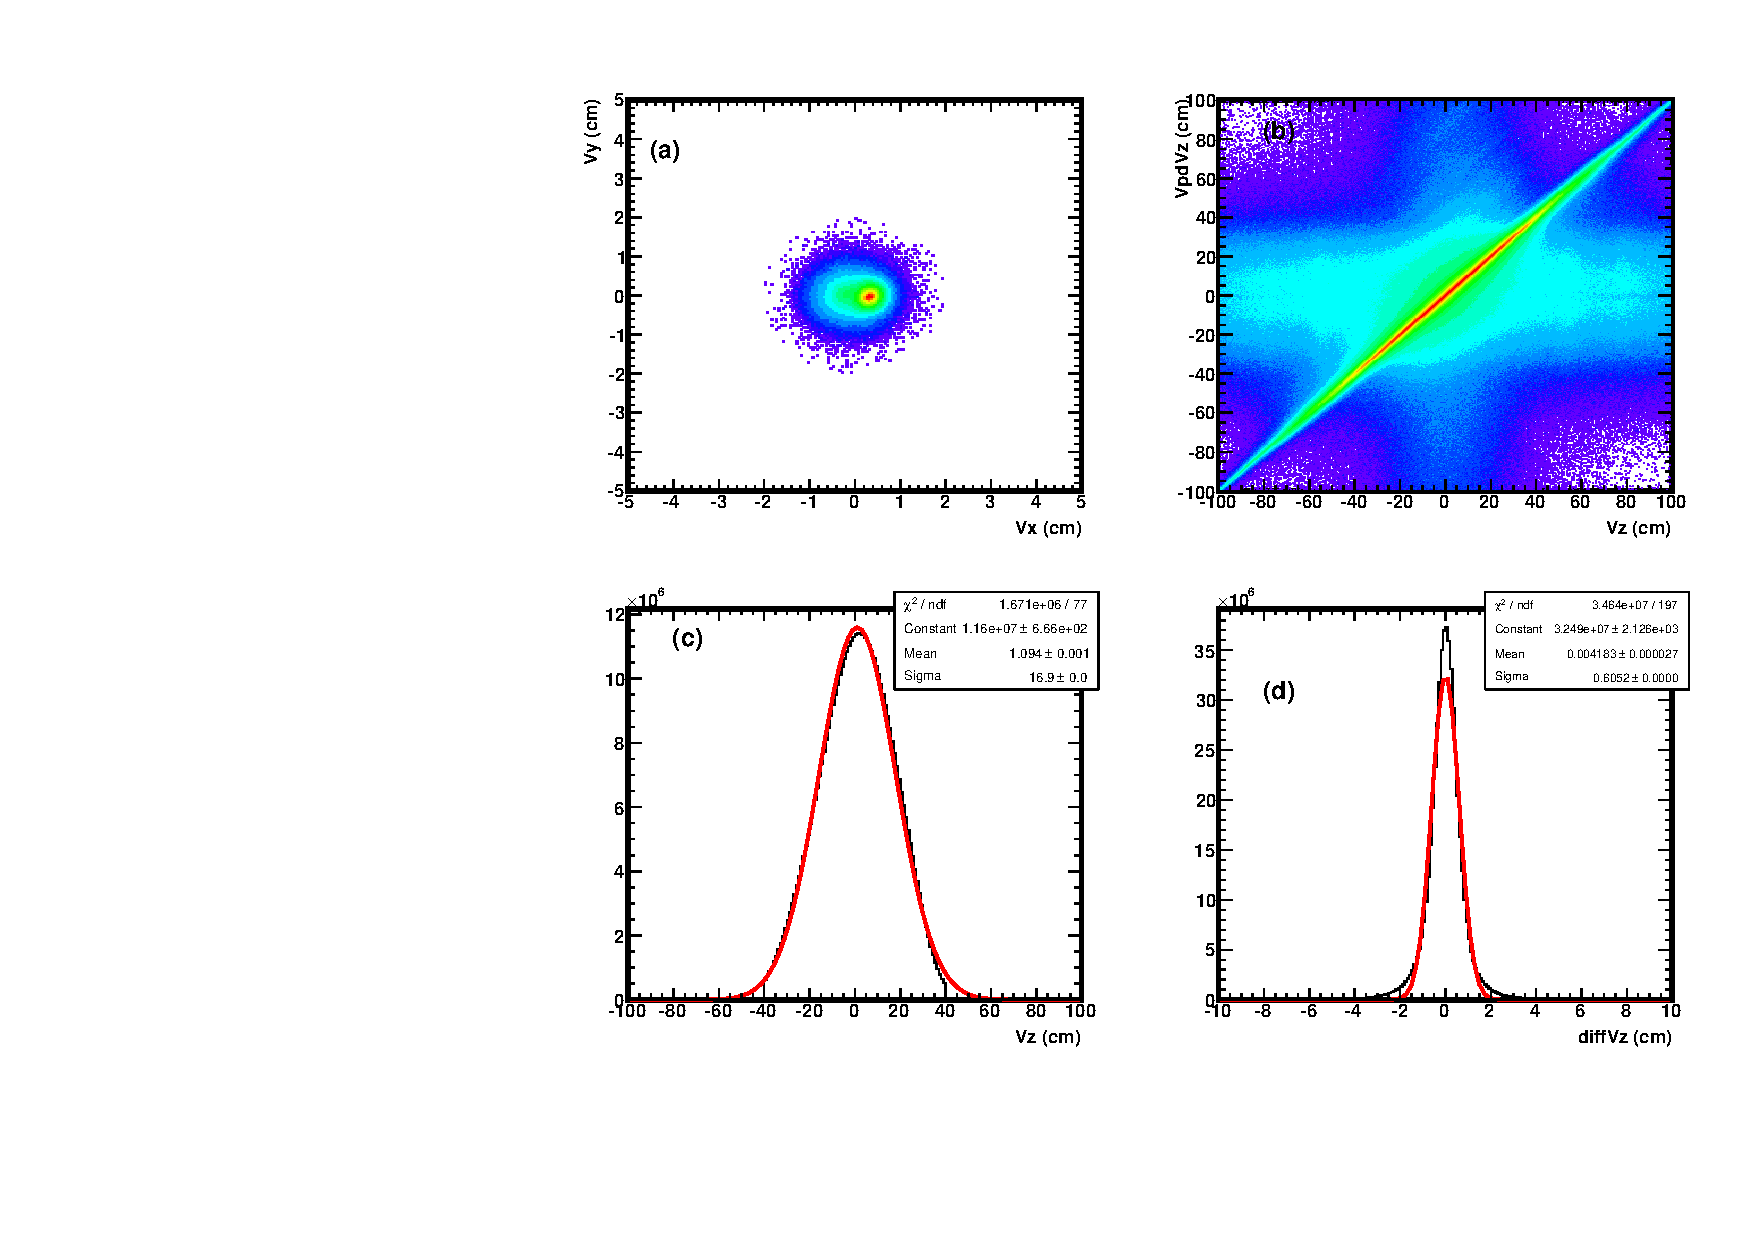
\includegraphics[angle=270,scale=0.7]{fig/3.Analysis/Additional/BasicQA/QA_fig1}
\par\end{centering}

\protect\caption{(a) TPC vertexR distribution, (b) TPC vertexZ and the VPD vertexZ
correlation, (c) TPC primary vertexX distribution, (d) difference
between TPC vertexZ and the VPD vertexZ in Au+Au 200 GeV minimum bias
collisions.}


\label{fig:vertex}
\end{figure}



\section{Centrality definition }

The centrality in Au+Au 200 GeV collisions was defined using the uncorrected
charged particle multiplicity $dN/d\eta$ within $|\eta|<0.5$ ( also
called reference multiplicity). A Monte Carlo Clauber calculation
was used to compared with the $dN/d\eta$ distribution from data to
define centrality bins. The dependence on collision vertex Z-position
and the luminosity has been also taken in account to address the efficiency
and acceptance change on the measured $dN/d\eta$. Figure \ref{fig:refmult}
shows the uncorrected $dN/d\eta$ distribution measured within $|Vz|<5cm$
and extrapolated to zero ZDC coincidence rate for the VPDMB triggered
events for Au+Au 200 GeV collision in year 2010 as well as the MC
Glauber simulation. The discrepancy at the low multiplicity is because
the VPD trigger efficiency starts getting lower while fewer particles
are produced. The difference in low multiplicity region has been taken
as a weight with the ration shown in Fig. \ref{fig:refmult} (bottom
panel) to account for the VPD inefficiency. Finally, the centrality
bins are defined according to the MC Glauder distribution to determine
the cut on the measured multiplicity. Table \ref{table:Npart Nbin Cen}
lists $\left\langle N_{part}\right\rangle $ and $\left\langle N_{bin}\right\rangle $
from the Glauber model simulation at $\sqrt{S_{NN}}=200GeV$ Au+Au.

\begin{figure}
\begin{centering}
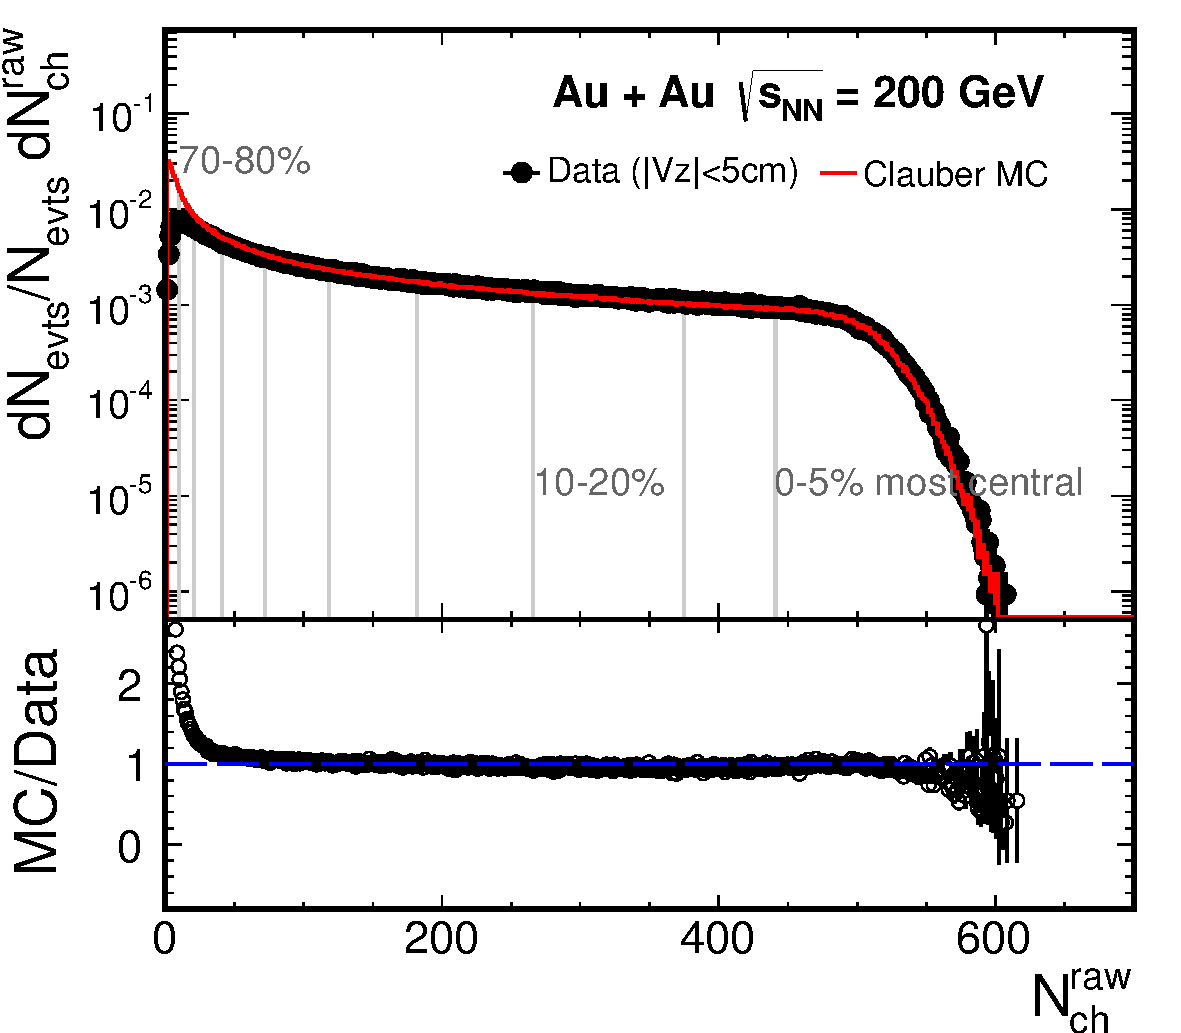
\includegraphics[scale=0.7]{fig/3.Analysis/Additional/dataset/paper_RefMult}
\par\end{centering}

\protect\caption{Upper Panel: Uncorrected charge particle multiplicity distribution
measured within $|\eta|<0.5$ and $|Vz|<5cm$. The red curve represents
the multiplicity distribution from MC Glauber calculation. Bottom
Panel: the ratio between MC and data.}


\label{fig:refmult}
\end{figure}


\begin{table}
\begin{centering}
\begin{tabular}{c|c|c}
\hline 
Centrality & $\left\langle N_{part}\right\rangle $ & $\left\langle N_{bin}\right\rangle $\tabularnewline
\hline 
\hline 
0-10\% & 325.5 ± 3.7 & 941.2 ± 26.3\tabularnewline
\hline 
10-40\% & 174.1 ± 10.0 & 391.4 ± 30.3\tabularnewline
\hline 
40-80\% & 41.8 ± 7.9 & 56.6 ± 13.7\tabularnewline
\hline 
\hline 
0-80\% & 126.7 ± 7.7 & 291.9 ± 20.5\tabularnewline
\hline 
\end{tabular}
\par\end{centering}

\protect\caption{Summary of centrality bins, average number of participants $\left\langle N_{part}\right\rangle $
and number of binary collisions$\left\langle N_{bin}\right\rangle $
from Monte Carlo Glauber simulation at $\sqrt{S_{NN}}=200GeV$ Au+Au
collision. }


\label{table:Npart Nbin Cen}
\end{table}



\section{Track selection and electron identification}


\subsection{Track selection}

Electron (including positrons if not specified) candidates are selected
from good tracks satisfied the flowing selection: 
\begin{enumerate}
\item number of fit points (\emph{nHitsFit}) in the TPC greater than 20
( maximum 45) to ensure good tracking quality and momentum resolution;
\item the ratio of number of fit points over number of possible fit points
in TPC greater than 0.52 to avoid split tracks in the TPC;
\item distance of closet approach (\emph{dca}) to the primary vertex less
then 1 cm to make sure selected tracks are from the primary collision;
\item number of \emph{dE/dx }points used for calculation average \emph{dE/dx
}greater than 16 to ensure good \emph{dE/dx} resolution.
\item with a valid matching to a TOF hit and projected position on TOF module
with the sensitive readout volume. 
\end{enumerate}
Table \ref{table:track and pid cut} left part lists the detailed
track quality cut.


\subsection{Electron identification}

In additional of track detection, momentum determination, TPC also
provide particle identification for charged particles by measuring
their ionization energy loss (\emph{dE/dx}) in the TPC gas. Usually,
a normalized \emph{dE/dx }(also called $n\sigma$) is used, which
is defined:

\begin{equation}
n\sigma_{e}=\frac{1}{R_{dE/dx}}ln\frac{\langle dE/dx\text{\ensuremath{\rangle}}{}^{Mea}}{\langle dE/dx\rangle_{e}^{Bichsel}}\label{eq:nsigmaE}
\end{equation}


in the Eq. \ref{eq:nsigmaE}: $R_{dE/dx}$ is the \emph{dE/dx} resolution,
\emph{Mea }and \emph{Bichsel} are measured value and theoretical value.
$n\sigma_{e}$ follows a standard gaussian distribution. 

With TPC only, however, it is difficult to separate electron from
hadrons because the electron band crosses with hadron bands in higher
momentum. With the flight timing information measured by TOF and the
track path-length measured from TPC, we can calculate the velocity
(β). Due to the very small electron mass, electron can be separated
from the slow hadron by the velocity cut. Combining the velocity (β)
information from TOF and energy loss(\emph{dE/dx}) from TPC, electron
can be identified up to momentum \textasciitilde{}3GeV/c. Figure \ref{fig:PID}
left panel shows the inverse velocity distribution as a function of
momentum, while the $n\sigma_{e}$ vs momentum distribution after
TOF velocity cut is shown in right panel. The detailed eID cuts are
listed in Table \ref{table:track and pid cut}.

\begin{table}[H]
\begin{centering}
\begin{tabular}{lr|lr}
\hline 
\multicolumn{2}{c|}{Track quality cuts} & \multicolumn{2}{c}{PID cuts}\tabularnewline
\hline 
\hline 
dca  & <1cm & $ $$p_{T}$  & > 0.2GeV/c\tabularnewline
nHitsFit  & >= 20 & $n\sigma_{e},p<1.0GeV/c$ $ $ & $1.5\times(p-1)-0.8\sim2.0$\tabularnewline
nHitsFit/nHitsPoss  & >=0.52 & $n\sigma_{e},p>1.0GeV/c$  & $-0.8\sim2.0$\tabularnewline
ndEdxFit  & >=16 & TOF $1/\text{β}$ & $|1-1/\text{β}|<0.025$ (Au+Au)\tabularnewline
η  & +/- 1 &  & $|1-1/\text{β}|<0.03$ (p+p)\tabularnewline
 &  & TOF yLocal &  $|yLocal|<1.8cm$\tabularnewline
\hline 
\end{tabular}
\par\end{centering}

\protect\caption{Electron selection criteria}
\label{table:track and pid cut}
\end{table}


\begin{figure}
\begin{centering}
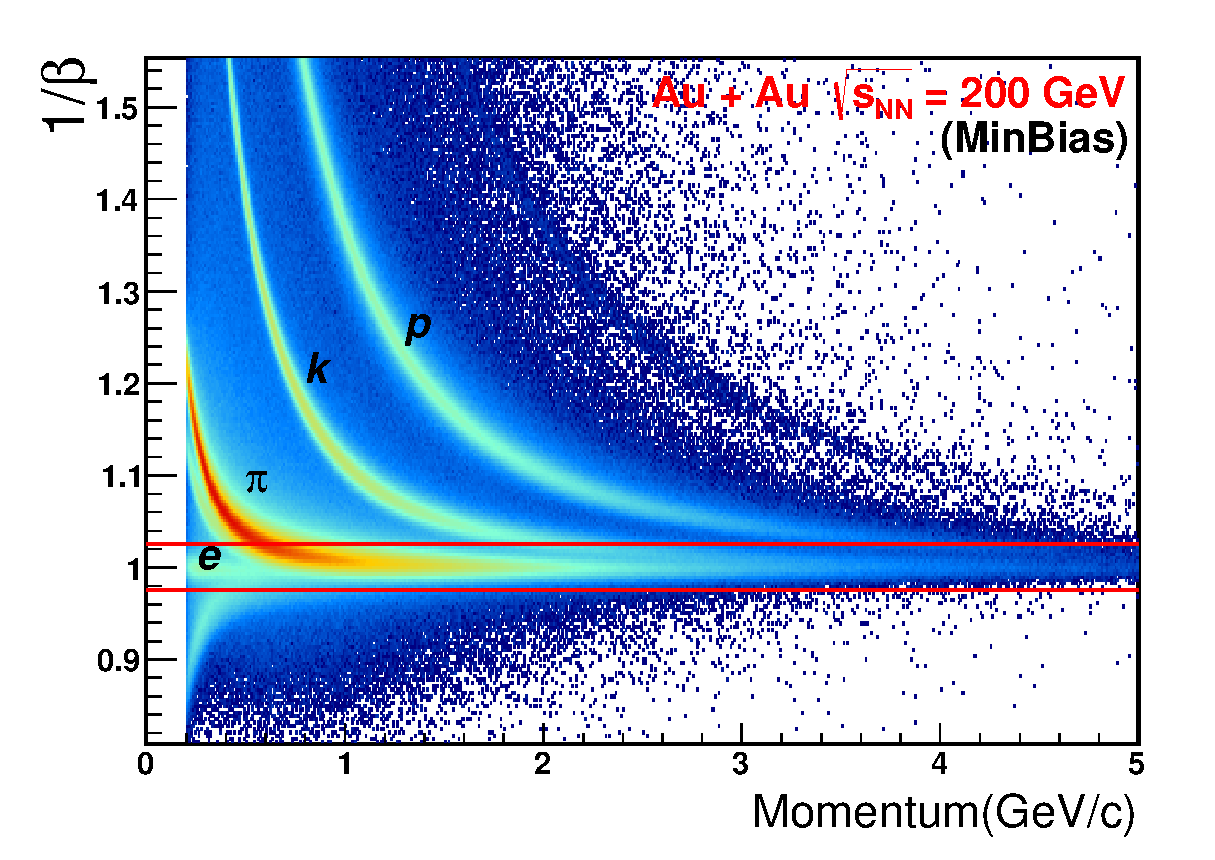
\includegraphics[scale=0.35]{fig/3.Analysis/Additional/PID/betavsp}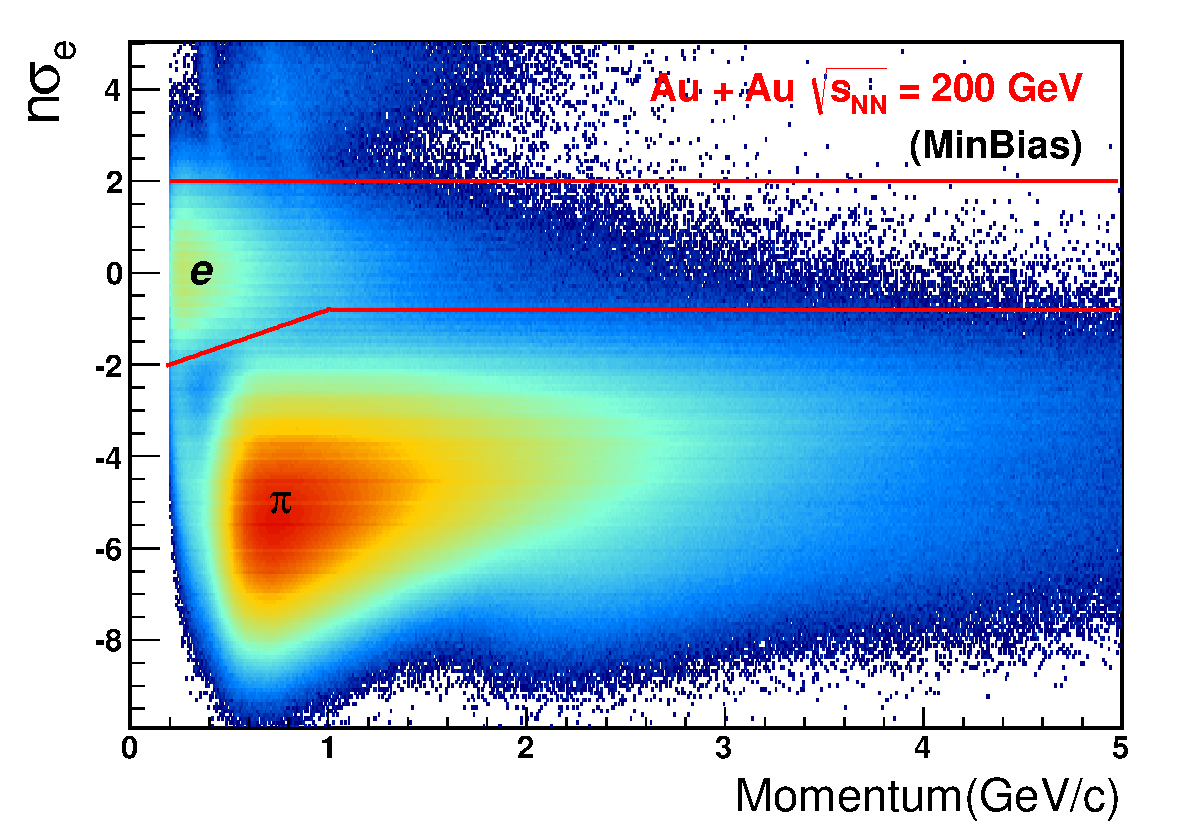
\includegraphics[scale=0.35]{fig/3.Analysis/Additional/PID/Nsigma_AuAu200}
\par\end{centering}

\protect\caption{Left panel: inverse velocity $1/\beta$ vs momentum distribution in
200GeV Au+Au collisions. Right panel: $n\sigma_{e}$ distribution
as a function of momentum after TOF velocity cut $|1/\beta-1|<0.025$
in 200GeV Au+Au collisions. The red lines in both panel show the PID
cuts.}


\label{fig:PID}
\end{figure}



\subsection{Hadron contamination and electron purity}

From Fig \ref{fig:PID} right panel, even after the TOF cut, the slow
hadron bands can still be seen in $n\sigma_{e}$ vs momentum. We selected
pure hadron ($\pi$, $k$ and $p$) sample by a very tight $m^{2}$
cut provided by TOF (shown in Fig \ref{fig: pure sample} left panel).
The pure electron sample was from photonic conversion and $\pi^{0}$
Dalitz decay (Fig \ref{fig: pure sample} (right)). This sample was
also used laterly in the efficiency study. Gaussian functions were
used to parameterize the $n\sigma_{e}$ distribution from the pure
sample for different particle species. Then, the hadron contamination
and electron purity were studied by multi-gaussian fit to the $n\sigma_{e}$
distribution in differential momentum bins to obtain the yields for
different particles. The mean and $\sigma$ were fixed in the fit
respecting to the value obtained from the pure sample. Figure \ref{fig:muli fit ex}
picks up the fit result in momentum bin {[}0.6, 0.64) GeV/c as an
example. The fit also included the merged $\pi$ component which is
from that the merging of two closed $\pi$ tracks, and has a doubled
\emph{dE/dx} value compared to a normal $\pi$ track. In some momentum
regions, the electron band crosses with the hadron bands, where the
multi-gaussian fit may not be reliable. In this analysis, exponential
functions were used to extrapolate the particle yields into the cross
region (Figure \ref{fig:yield and purity} (left), and the uncertainties
from the exponential fit were taken into account as systematic uncertainty.
Figure \ref{fig:yield and purity} right panel shows the electron
purity for Au+Au 200GeV minimum bias data taken in year 2011. Table
\ref{Table:purity} lists electron purity for the data set used in
this analysis.

\begin{figure}
\begin{centering}
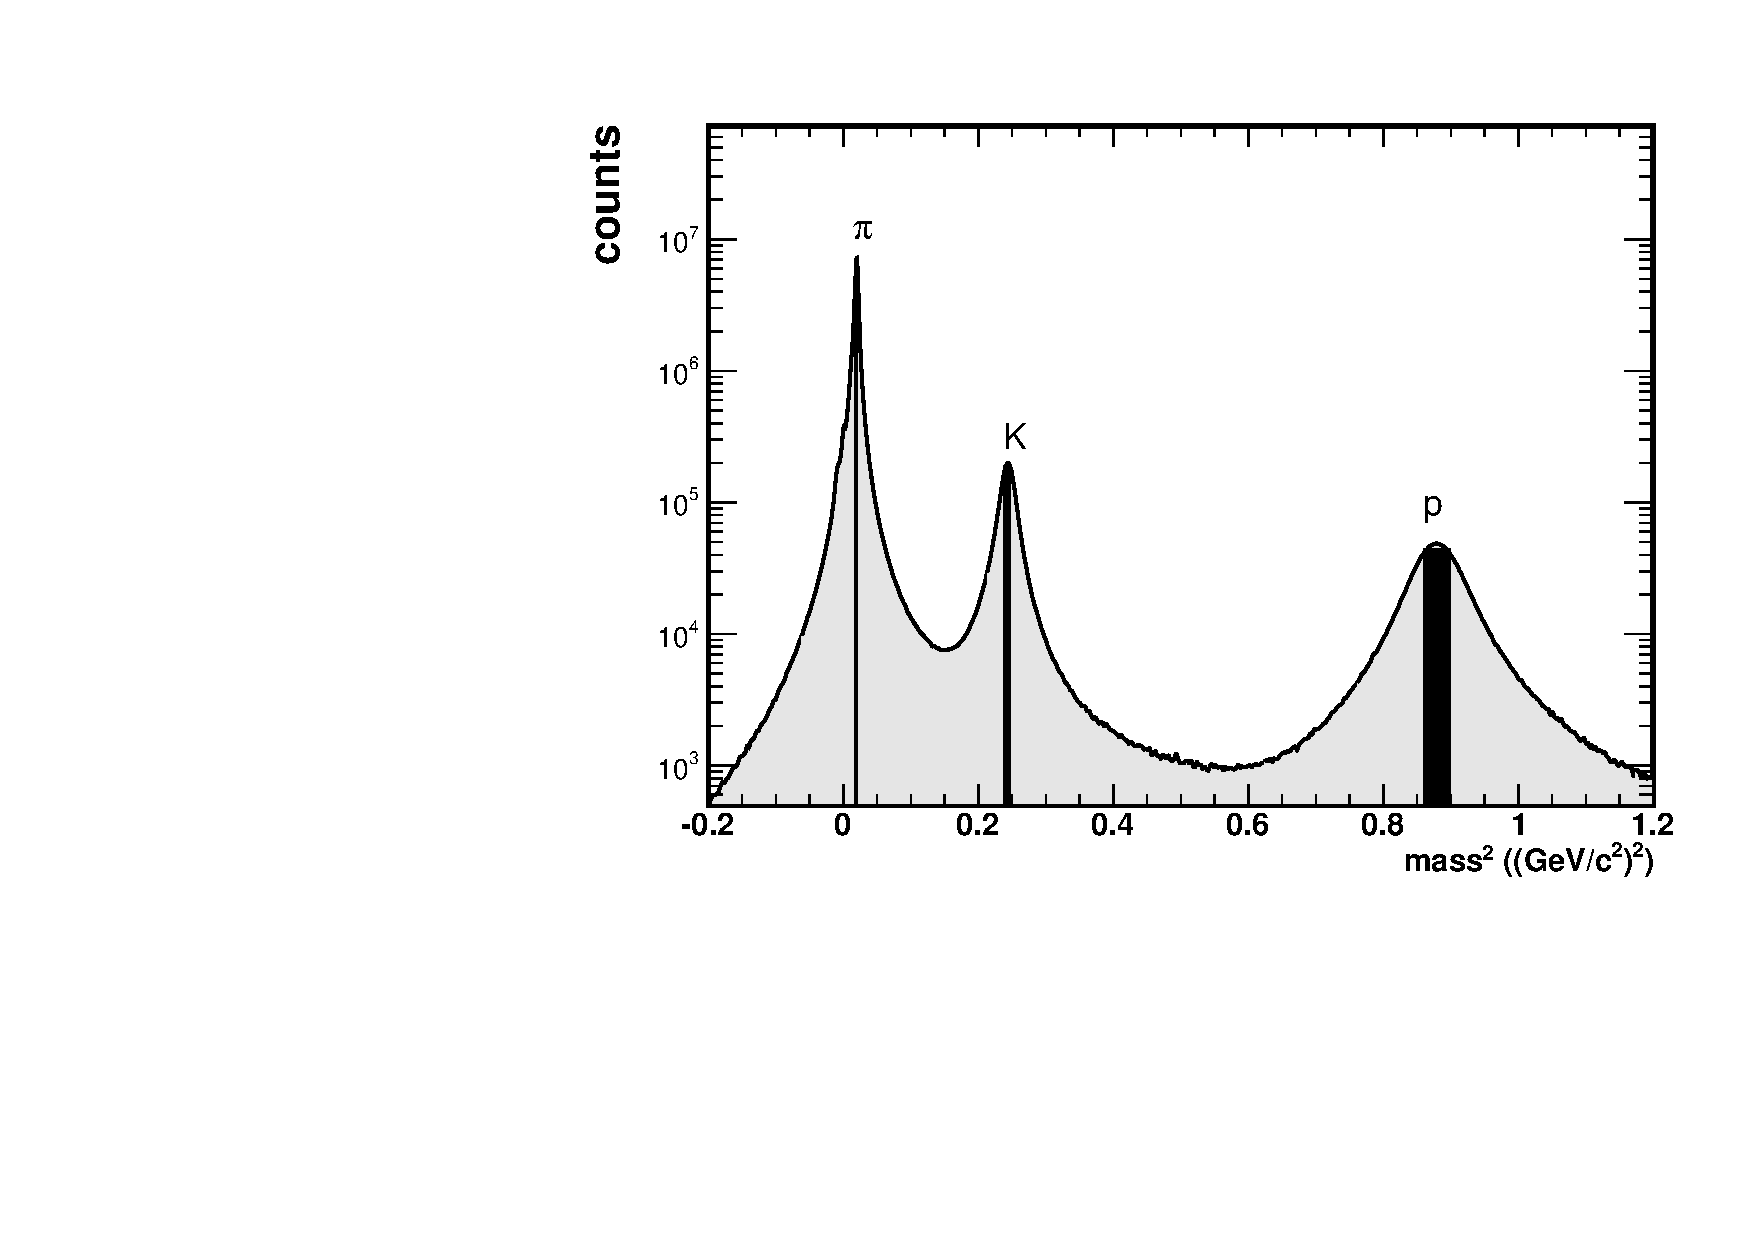
\includegraphics[angle=270,scale=0.35]{fig/3.Analysis/Additional/BasicQA/QA_fig3}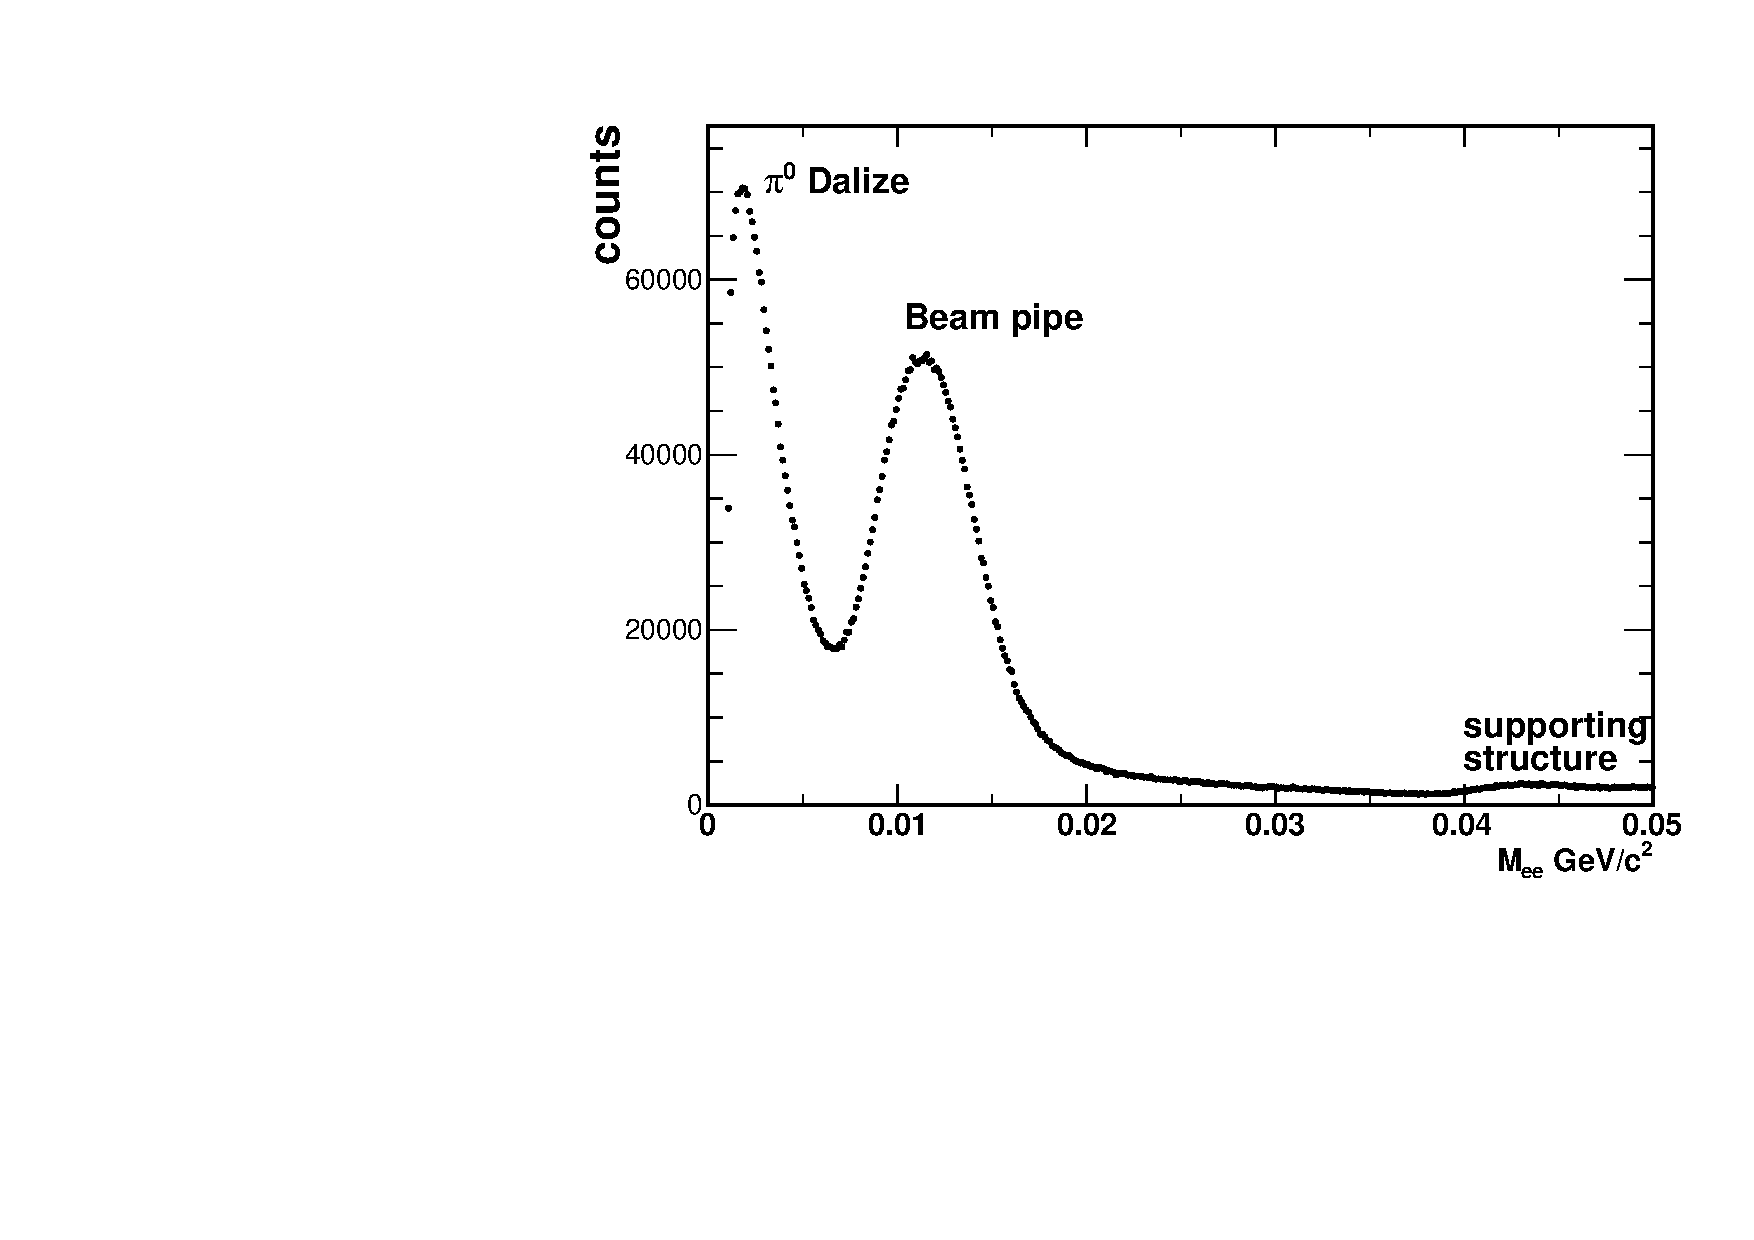
\includegraphics[angle=270,scale=0.35]{fig/3.Analysis/Additional/purity/fig5}
\par\end{centering}

\protect\caption{Left panel: Hadron sample selected by TOF. Right panel: pure electron
sample from $\pi^{0}$ Daliza decay and photonic conversion.}


\label{fig: pure sample}
\end{figure}


\begin{figure}
\begin{centering}
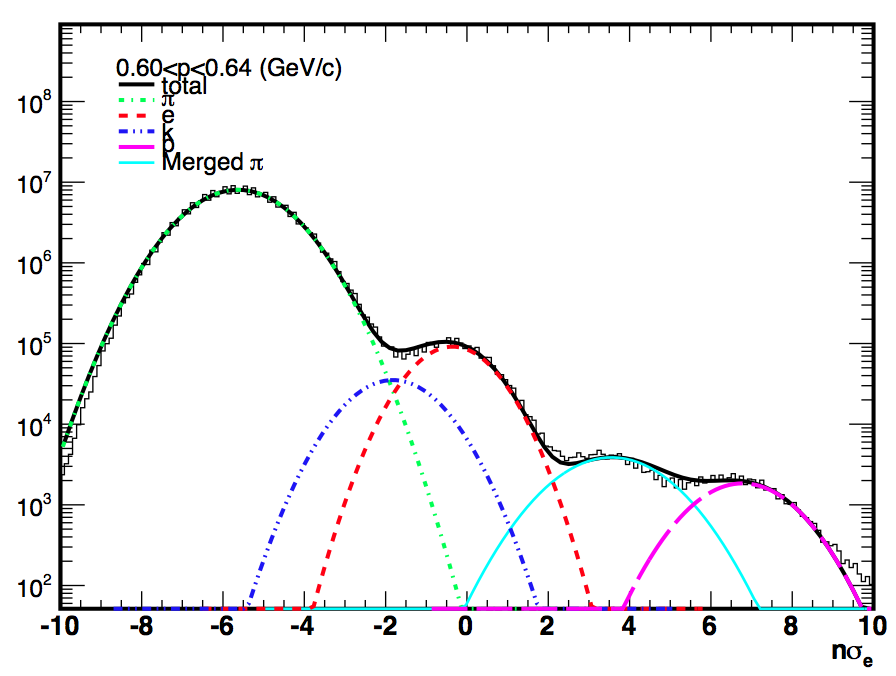
\includegraphics[scale=0.4]{fig/3.Analysis/Additional/purity/muliFit}
\par\end{centering}

\protect\caption{A multi-gaussian fit in momentum bin {[}0.6, 0.64) (GeV/c) in Au+Au
200GeV minimum bias collisions. }


\label{fig:muli fit ex}
\end{figure}


\begin{figure}
\begin{centering}
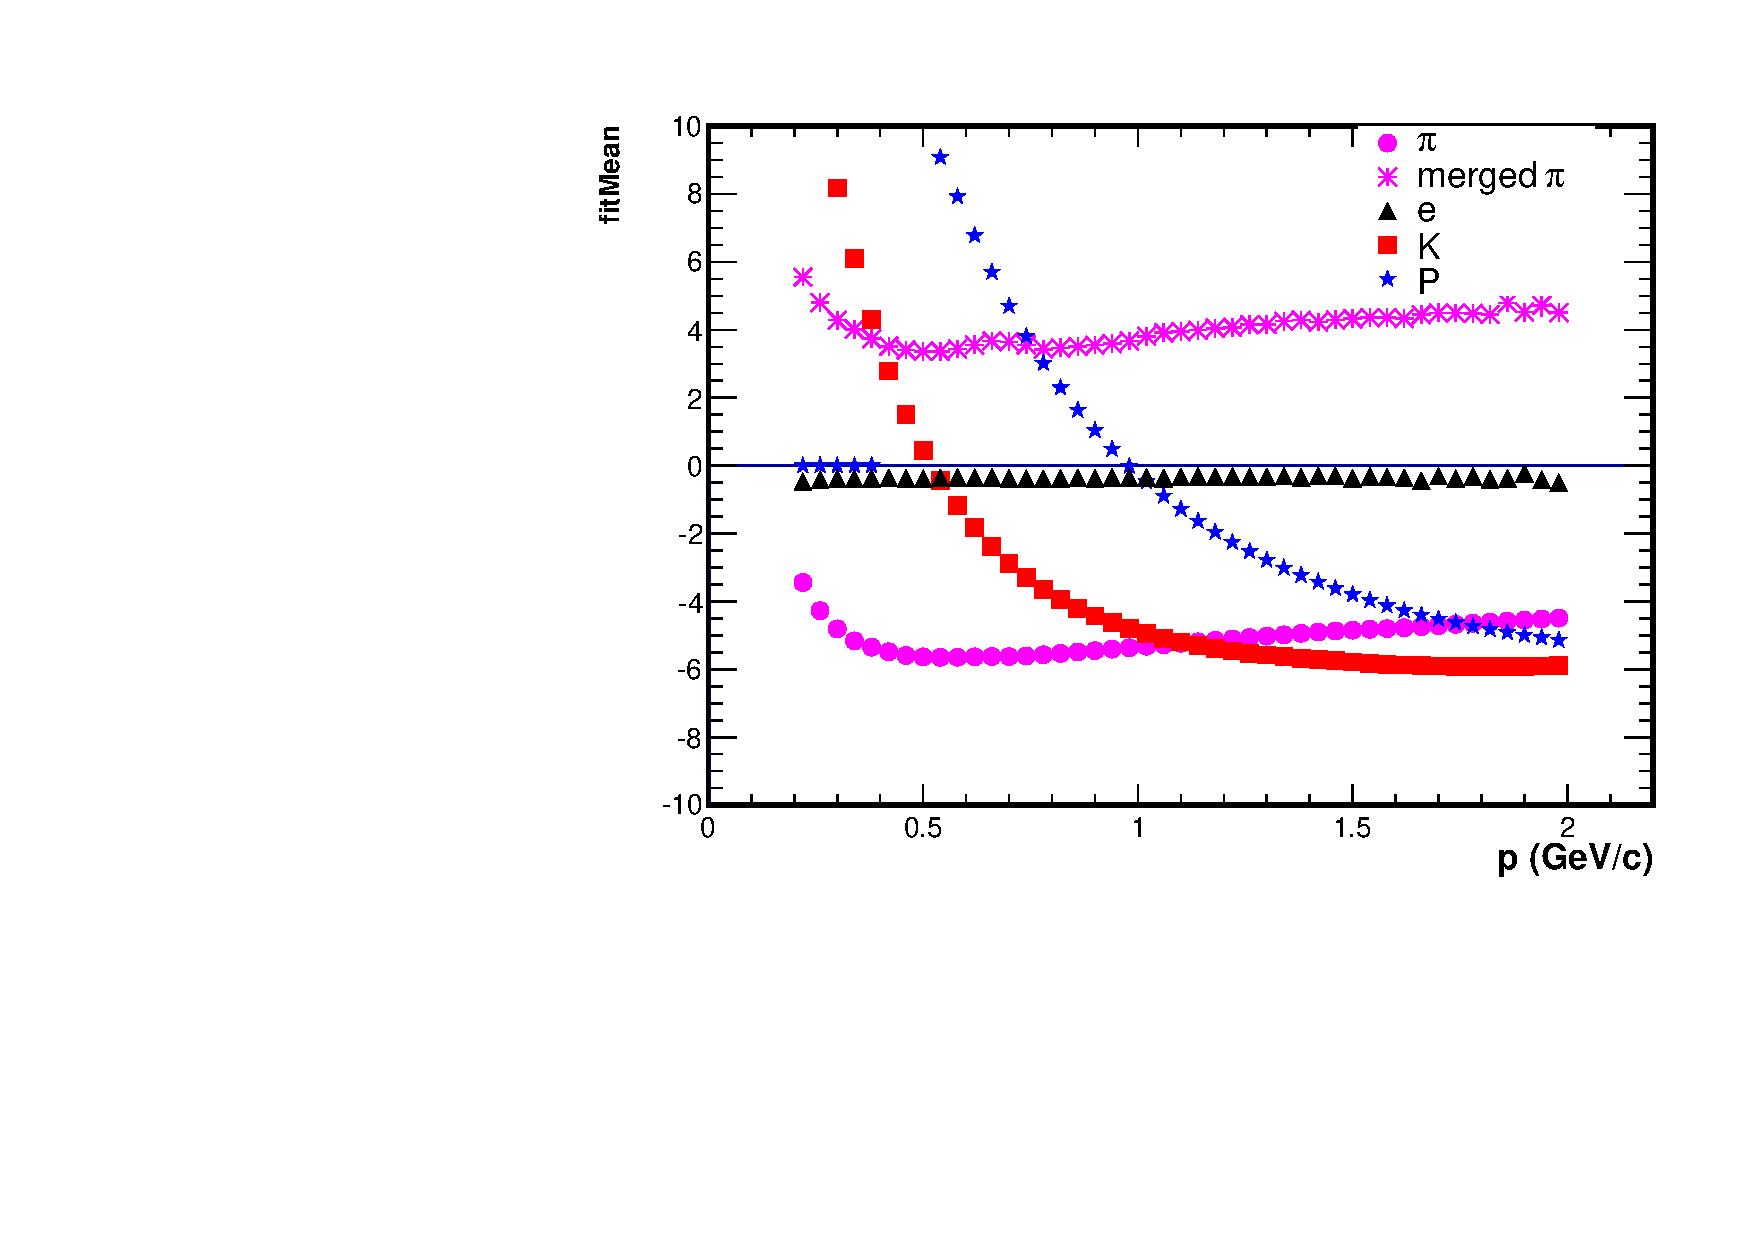
\includegraphics[angle=270,scale=0.35]{fig/3.Analysis/Additional/purity/mean3}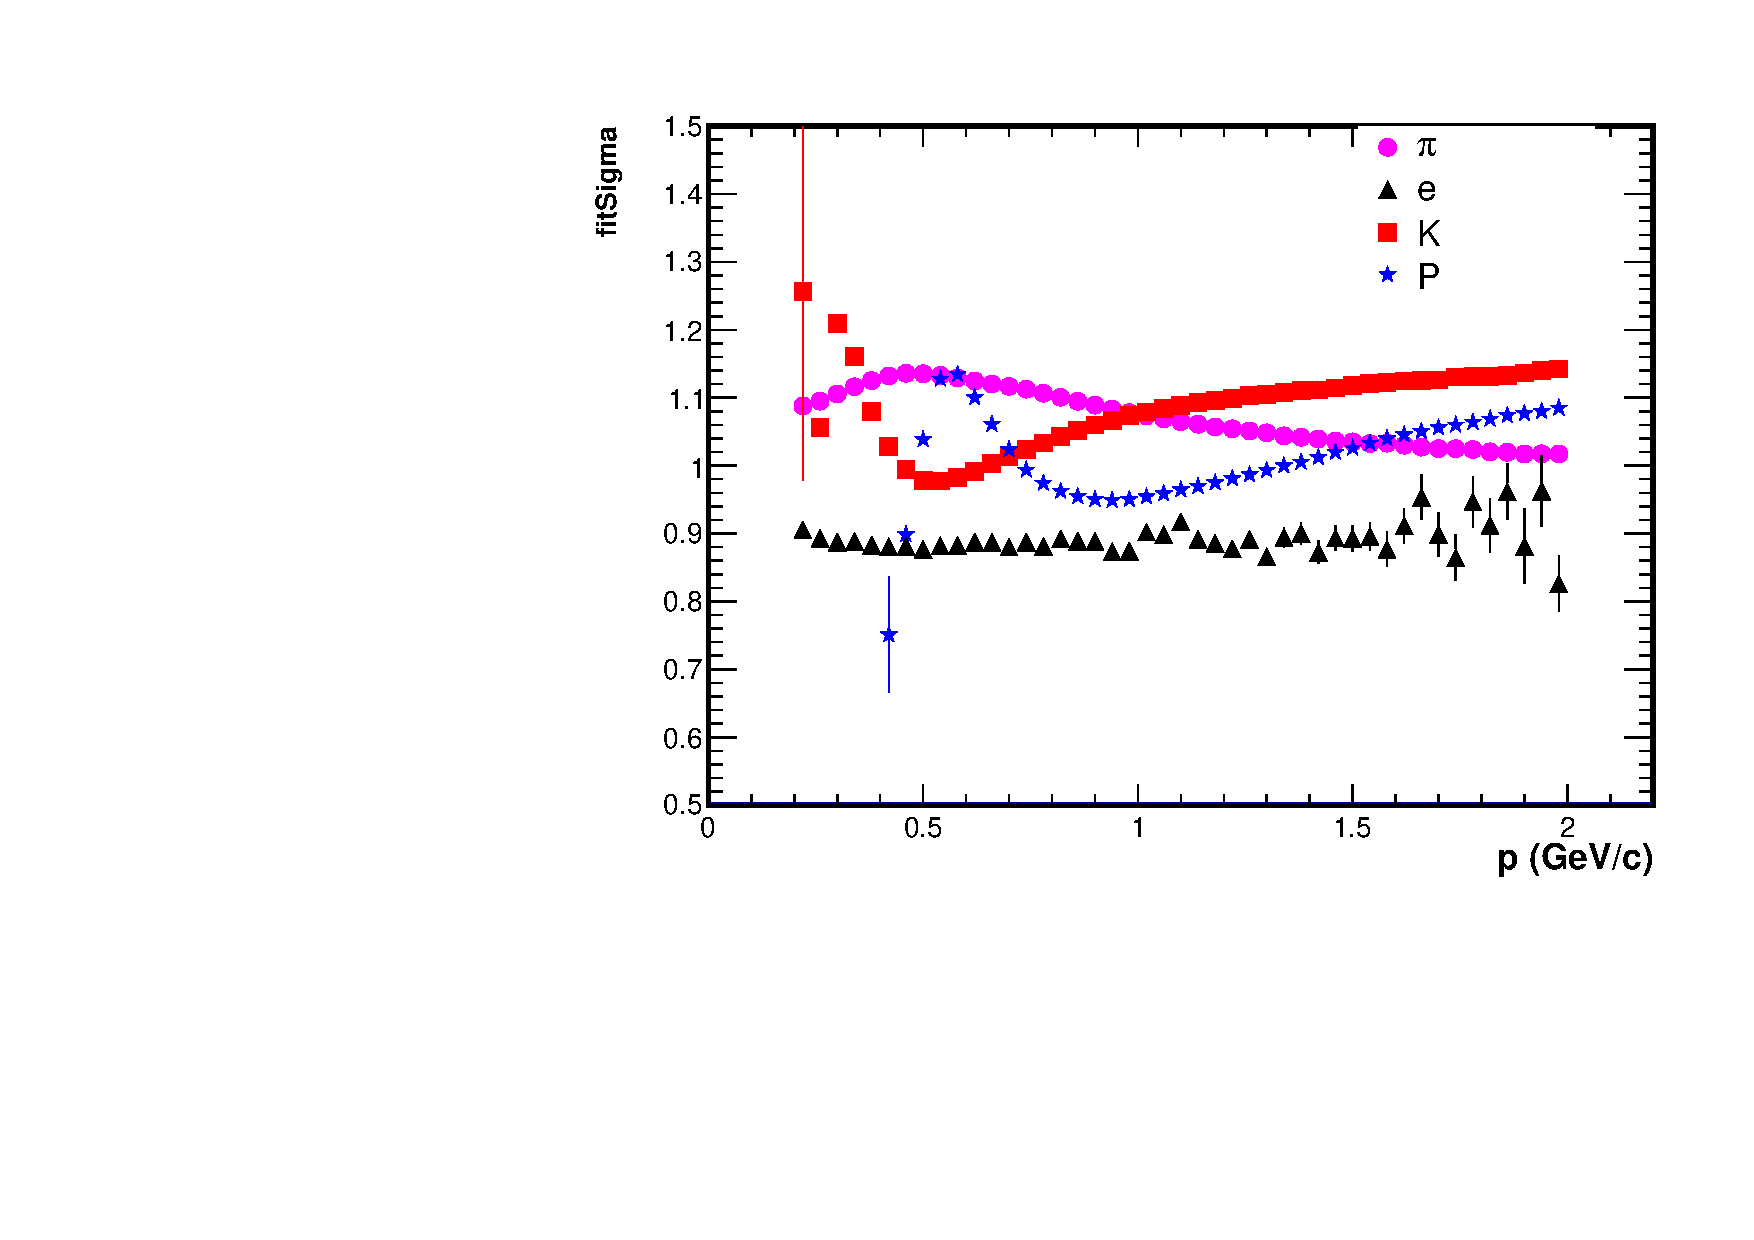
\includegraphics[angle=270,scale=0.35]{fig/3.Analysis/Additional/purity/sigma3}
\par\end{centering}

\protect\caption{Mean (left) and sigma (right) of the gaussian distribution as a function
of momentum from pure samples for different particle species in Au+Au
200GeV minimum bias collisions.}


\end{figure}


\begin{figure}
\begin{centering}
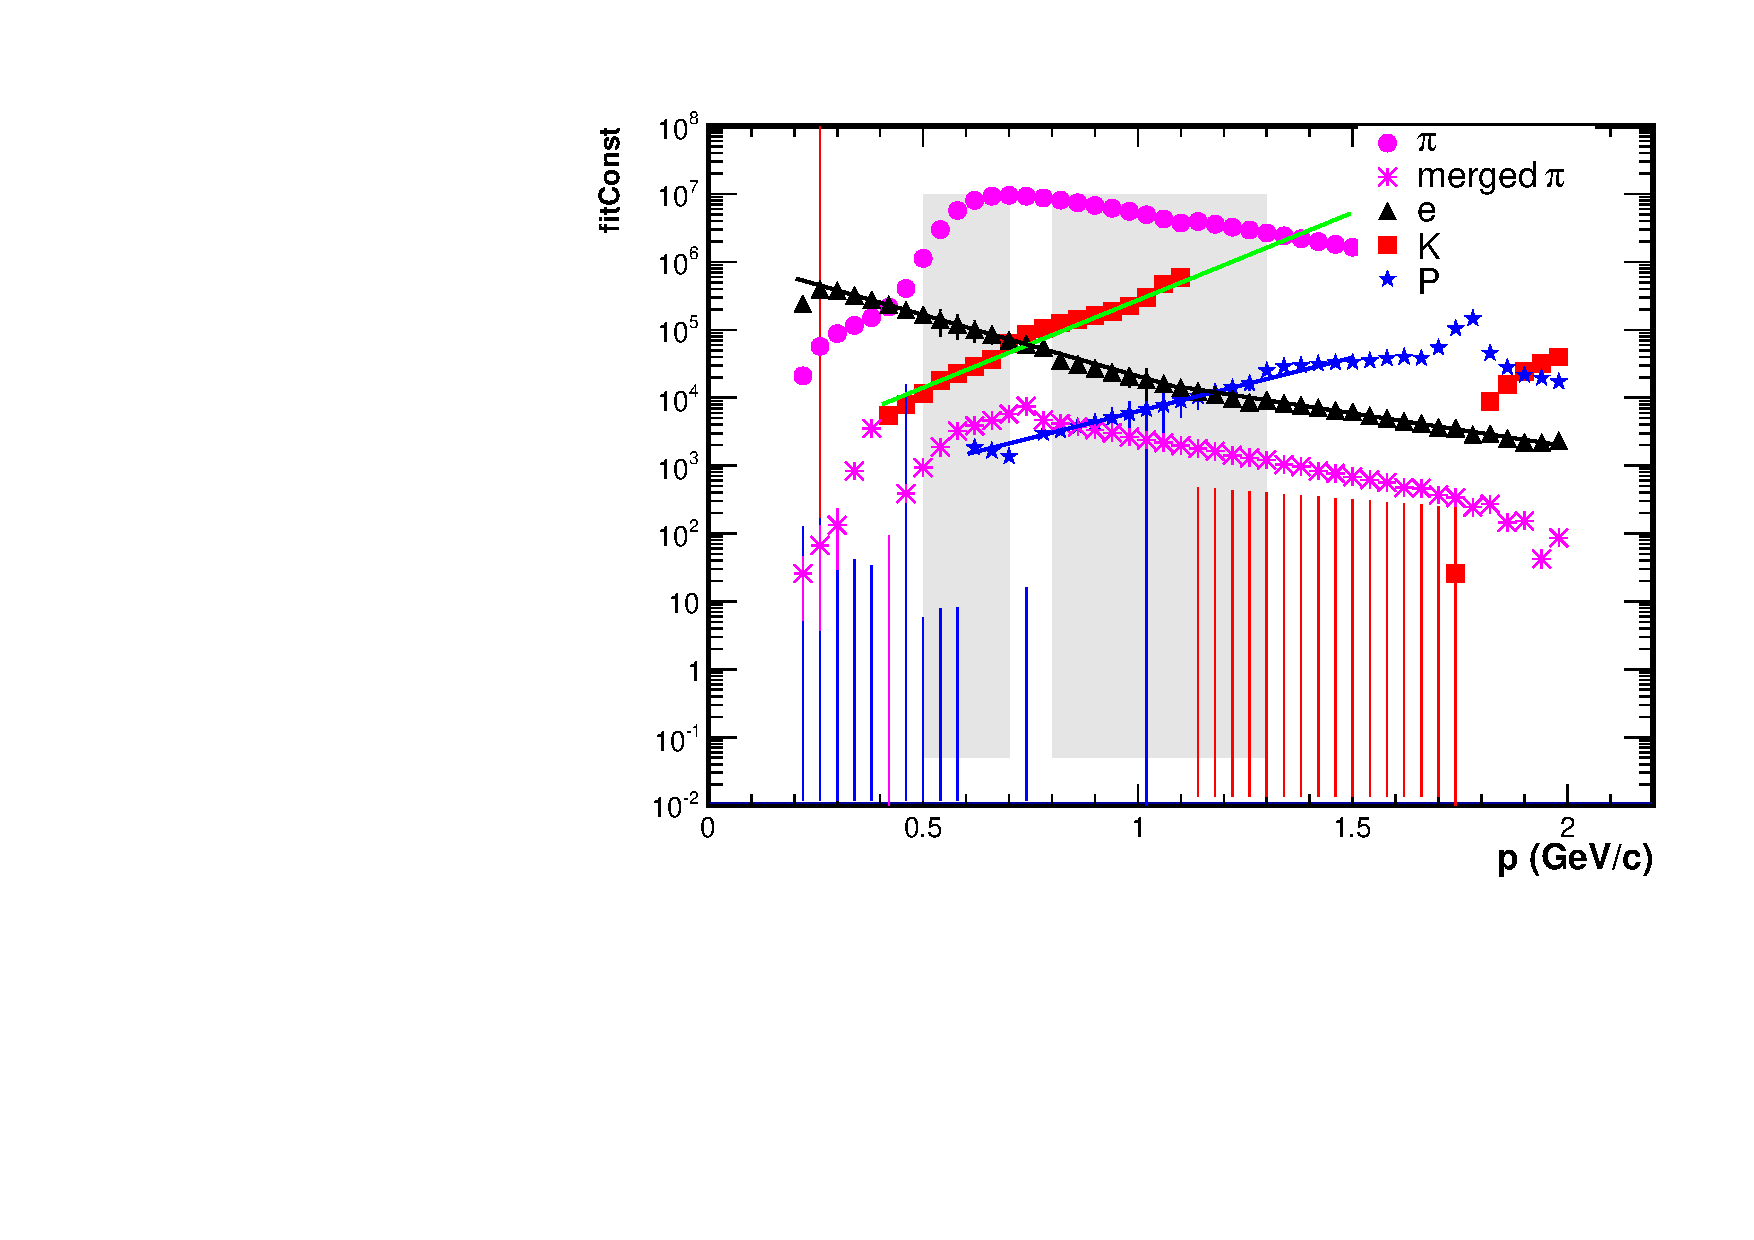
\includegraphics[angle=270,scale=0.35]{fig/3.Analysis/Additional/purity/const3}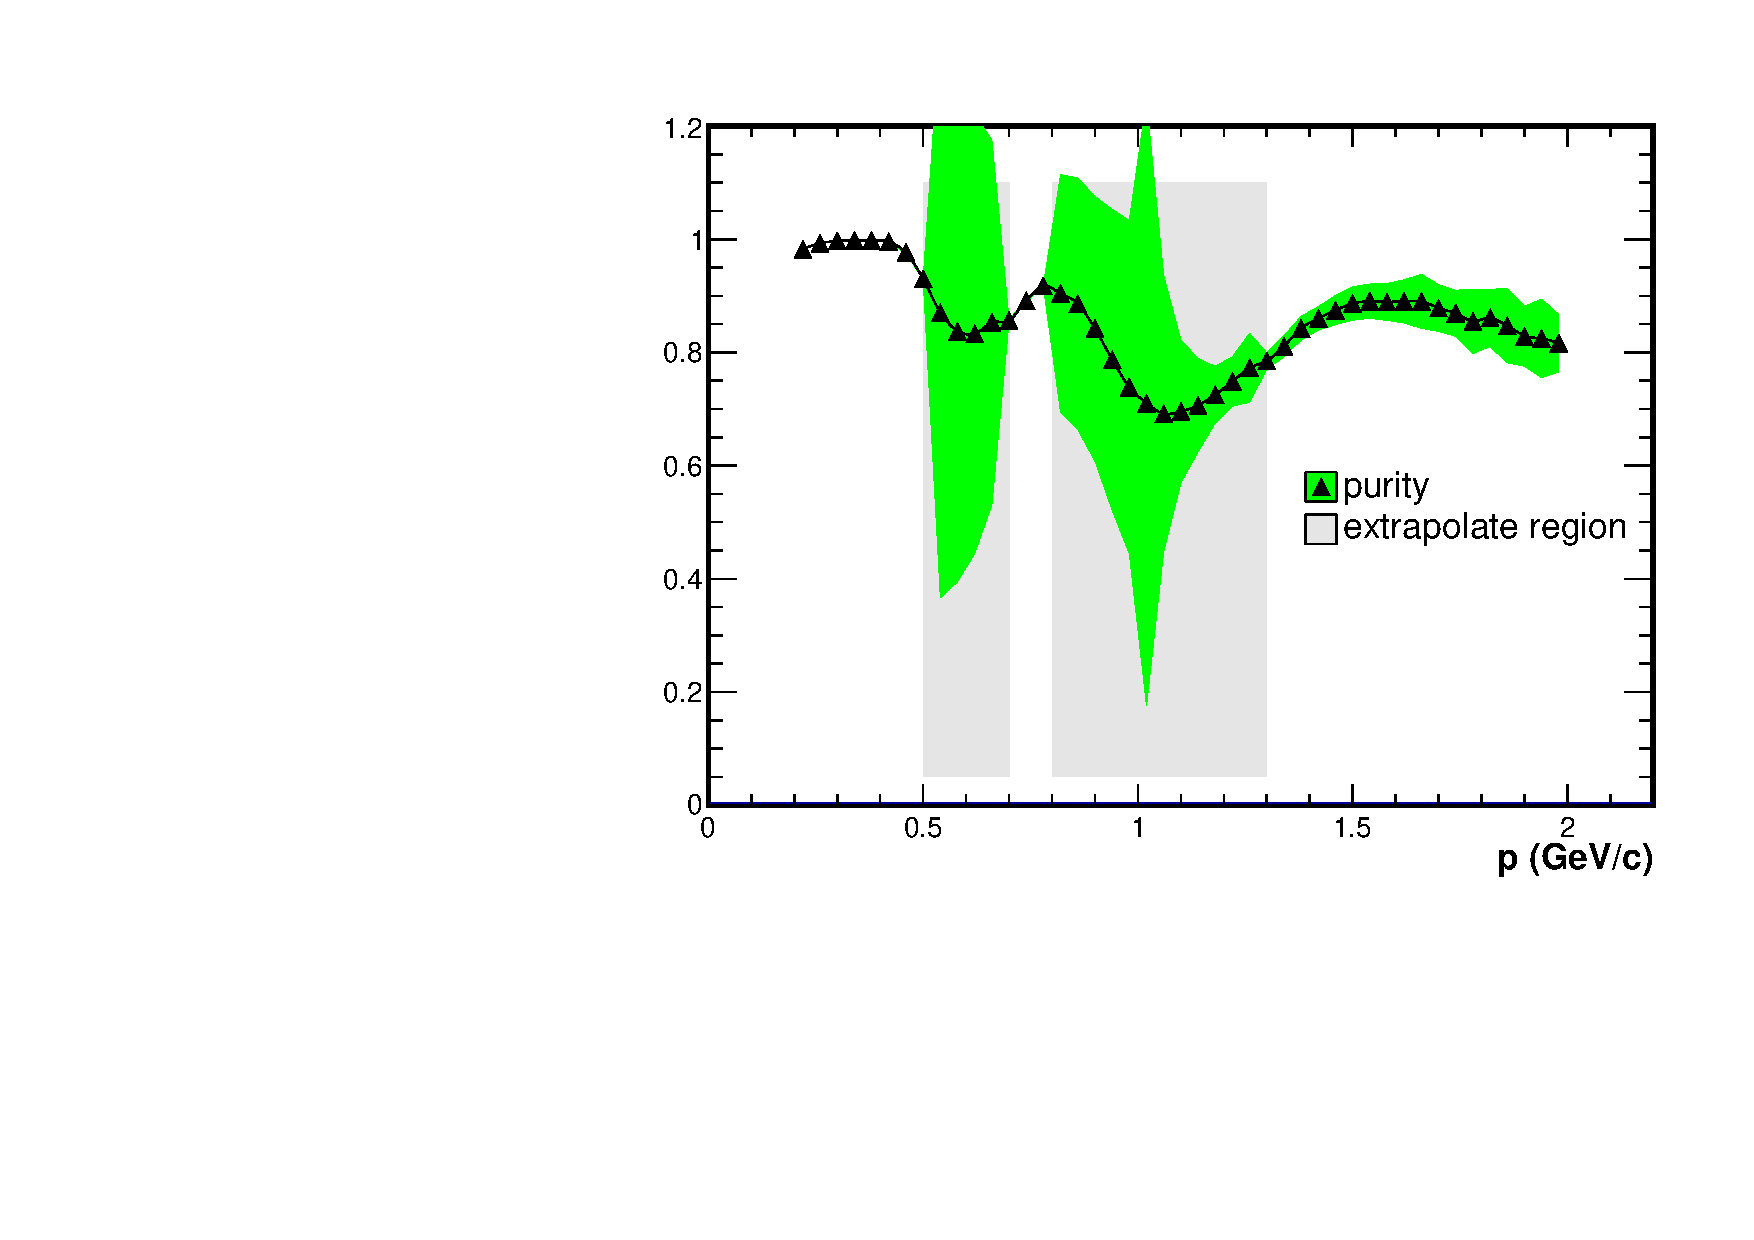
\includegraphics[angle=270,scale=0.35]{/Users/luthien/Documents/Thesis/Thesis/fig/3.Analysis/Additional/purity/eff_purity_3}
\par\end{centering}

\protect\caption{(left) Yields for different particle species from multi-gaussian fit
as a function of momentum. The grey area show the cross region. And
the solid lines depict the exponential fits to extrapolate the yields
in the cross region. (right) Electron purity as a function of momentum,
the green band represents he uncertainty from the extrapolation and
the multi-gaussian fits.}


\label{fig:yield and purity}
\end{figure}

\begin{lyxcode}
\begin{table}
\begin{centering}
\begin{tabular}{c|c|c}
\hline 
Au+Au 200GeV & MinBias & $\sim0.946\pm0.024$\tabularnewline
\hline 
 & Cenrtral & $\sim0.921\pm0.025$\tabularnewline
\hline 
p+p 200GeV & MinBias & $\sim0.980\pm0.040$\tabularnewline
\hline 
\end{tabular}
\par\end{centering}

\protect\caption{Electron purity for different data samples.}


\label{Table:purity}

\end{table}

\end{lyxcode}

\section{Pair reconstruction and background}

The dielectron pairs (foreground, also marked as \emph{unlike-sign
pairs}) were reconstructed by randomly combining electron and position
from the high purity electron (position) sample from the same event.
The invariant mass of di-electron pairs $M_{ee}$ were calculated
as :

\begin{equation}
M_{ee}=\sqrt{(E_{+}+E_{-})^{2}-(\overset{\rightarrow}{p_{+}}+\overset{\rightarrow}{p_{-}})^{2}}
\end{equation}


where $E_{\pm}=\sqrt{(\overset{\rightarrow}{p_{\pm}})^{2}+m_{e}^{2}}$,
$m_{e}=0.511MeV/c$, and $\overset{\rightarrow}{p_{\pm}}$ is the
momentum of electron (positron) which was measured by TPC. The candidate
tracks were required to satisfy cut: $p_{T}>0.2GeV/c$ and $|\eta|<1$
to fit into the acceptance of STAR detector, while the dielectron
pairs were constructed in mid-rapidity ($|y_{ee}|<1$). Unlike-sign
pairs include the dielectron signal and background, where the signal
is defined by dielectron pairs from hadron decay, and QGP/media contribution
which is what we are interested . On the other hand, the background
includes the following source:
\begin{enumerate}
\item Combinatorial background: background come from randomly pairing, which
is uncorrelated.
\item Correlated background, which is the case that two partner tracks come
from different parents but from the same source. E.G, $\pi^{0}\rightarrow\gamma+e^{+}e^{-}$,
then $\gamma$ converts into another $e^{+}e^{-}$ pair, when pair
is combined randomly, it is possible to pick one track from $\pi^{0}$
decay and another from the converted $ $photon. There is also contribution
from Jet, e.g electrons and positrons from same Jet or back to back
Jet. In this case, the final state particles are correlated, which
is mainly contributed in high momentum and high mass region. In additional,
the hadron contamination also has small contribution, e.g $\pi$,
$p$ from $\Lambda$ decay are misidentified by electrons. This contribution
was considered as systematic uncertainty, and will be discussed in
following section.
\item Photon conversion. The invariant mass of dielectron pairs from real
photon conversion should be 0. However, due to the primary track reconstruction
algorithm, the momentum of these electrons from conversion which happened
away from the primary vertex are biased, which lead to a finite pair
invariant mass. This kind of background mainly contributes in very
low mass region ($M_{ee}<0.2GeV/c^{2}$). It will be discussed in
detail in follow section.
\end{enumerate}
In this analysis, we adopted two methods to reproduce the background.


\subsection{Like-sign method}

The Like-sign method is used to calculate contributions of uncorrelated
and correlated background at the same time and serves as a standard
of the background to justify the background distribution. In this
analysis, we constructed like-sign background by randomly combining
same charge pairs $N_{++}$ , $N_{--}$ from the same event. We used
the geometric mean of the like-sign pairs $2\sqrt{N_{++}\times N_{--}}$
, because it is demonstrated in this paper \cite{PhysRevC.81.034911}
that when the $e^{+}$ and $e^{-}$ are produced in statistically
independent pairs, the geometric mean fully describes the background
in the unlike-sign pair foreground distribution.

The TPC detector has de-active zones, (e.g the gap between TPC sectors),
and in magnet field, different charged particles are bended into opposite
direction. Therefore, the acceptance of different charged particle
is different. Figure \ref{fig:pmaccTPC} shows the transverse momentum
($p_{T}$) vs azimuthal angle ($\phi$) distribution of negative tracks
and positive tracks in magnet field. The white bands show the de-active
regions of TPC. In Figure \ref{fig:pmaccTPC}, it can be clearly seen
that the acceptance effect is different for negative and positive
charged tracks. So due to the acceptance effect, the acceptance of
unlike-sign pairs and like-sign pairs are different (Fig \ref{fig:accdiff}). 

To address this difference, mixed event method was used in this analysis.
Due to it does not include correlated pairs, mixed event method can
be used to study the detector acceptance effect. The like-sign background
was calculated by Eq. \ref{eq:LSacc}, and the acceptance correction
factor also defined there. The $p_{T}$ dependence was also considered
by applying a 2D ($ $mass vs $p_{T}$) acceptance factor correction,
and the difference between 2D and 1D was included in systematic uncertainty.
Figure \ref{fig:accfactor} shows acceptance correction factor as
function of $M_{ee}$ in 200 GeV Au+Au and p+p minimum bias collisions.

\begin{align}
N_{likesign}(M_{ee},p_{T}) & =2\sqrt{N_{++}(M_{ee},p_{T})\times N_{--}(M_{ee},p_{T})}\cdot F_{acc}(M_{ee},p_{T})\nonumber \\
F_{acc}(M_{ee},p_{T}) & =\frac{N_{+-}^{Mix}(M_{ee},p_{T})}{2\sqrt{N_{++}^{Mix}(M_{ee},p_{T})\times N_{--}^{Mix}(M_{ee},p_{T})}}\label{eq:LSacc}
\end{align}


\begin{figure}
\begin{centering}
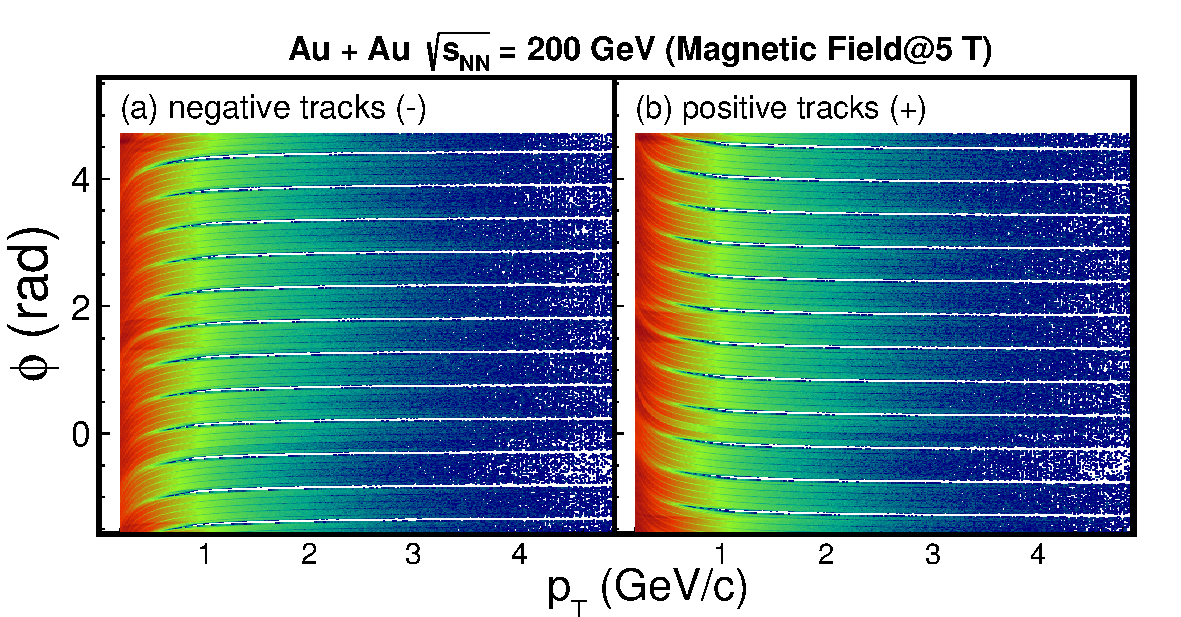
\includegraphics[width=0.8\textwidth]{fig/3.Analysis/Additional/paper_phiAcc_star}
\par\end{centering}

\protect\caption{$p_{T}$ vs $\phi$ distribution for negative tracks (a) and positive
tracks (b) in magnet field.}


\label{fig:pmaccTPC}

\end{figure}


\begin{figure}
\begin{centering}
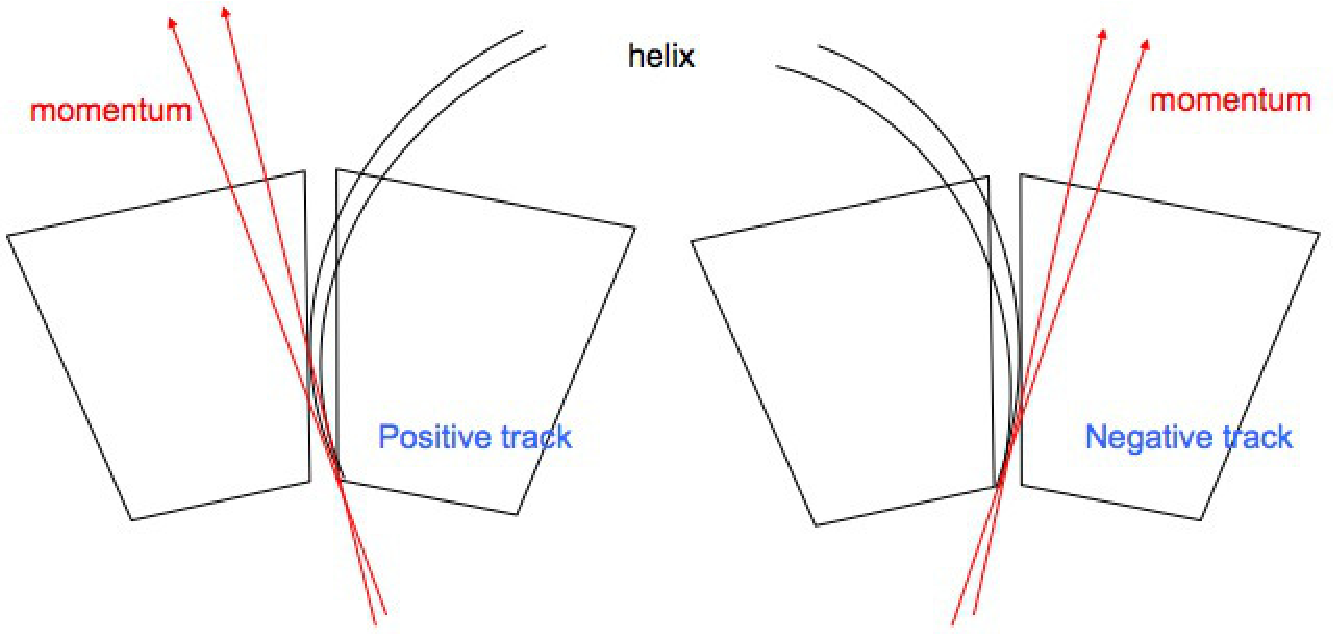
\includegraphics[width=0.8\textwidth]{fig/3.Analysis/background/Acc1}
\par\end{centering}

\begin{centering}
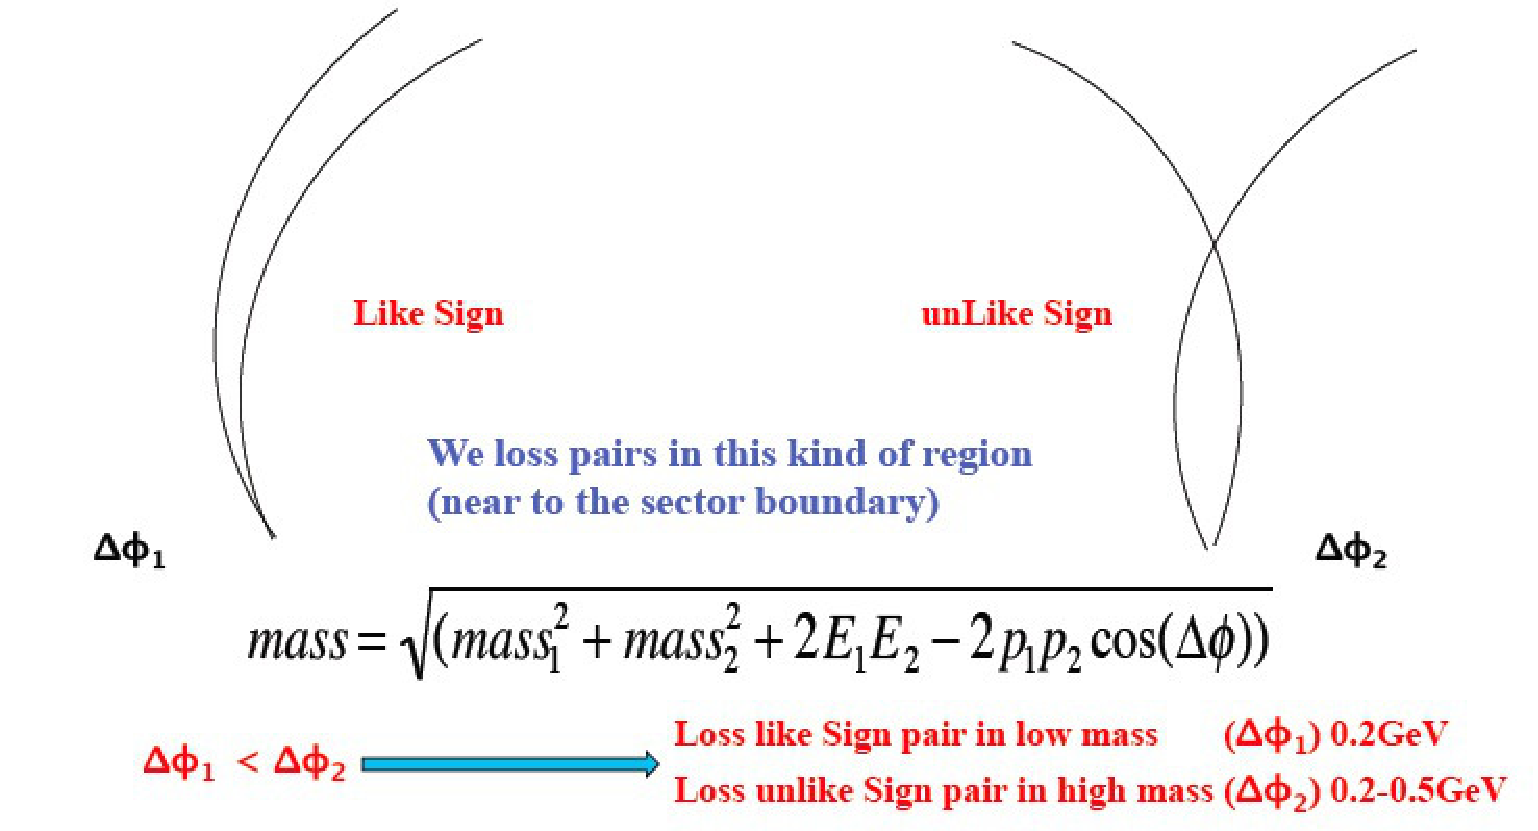
\includegraphics[width=0.8\textwidth]{fig/3.Analysis/background/Acc2}
\par\end{centering}

\protect\caption{A cartoon shows the acceptance difference between unlike-sign pairs
and like-sign pairs.}


\label{fig:accdiff}

\end{figure}


\begin{figure}
\begin{centering}
\includegraphics[width=0.5\textwidth]{fig/3.Analysis/background/AuAu/paper_Acc}\includegraphics[width=0.5\textwidth]{fig/3.Analysis/background/pp/paper_Acc}
\par\end{centering}

\protect\caption{(left) Acceptance correction factor in Au+Au 200 GeV collision. (right)
Acceptance correction factor in p+p 200GeV collision.}


\label{fig:accfactor}
\end{figure}



\subsection{Mixed event method}

Like-sign method as mentioned in section 3.4.1 can fully reproduce
combinatorial background and correlated background. However, the like-sign
background is leak of statistics. In this analysis, the like-sign
background was used in low mass region where we have better statistics.
For higher mass region, event mixing technique was used to achieve
better statistical accuracy. 

Mixed event background is reproduced by mixing electron candidate
tracks from different event. Since the two tracks are uncorrelated,
mixed event method is only able to reconstruct combinatorial background.
To ensure events mixed together have similar structure, we classified
event sample according magnet, centrality, Vz and event plane, and
split it into $Magnet\times Centrality\times EventPlane\times Vz=2\times9\times12\times10$
event pools. Each event pool holds 50 (100 for p+p data) events at
maximum, when the number of events in the event pool reach limitation,
one event is randomly dropped to make space for the new coming events.
Dr. Jie Zhao did very detailed study about the number of event pools
and event buffer effect on mixed event background in \cite{Zhao:2013vn}.
Here we chosen the number of event pools and event buffer respecting
to his study.

The mixed event background should be normalized to the same amplitude
of like-sign background, since the like-sign background can fully
reproduce the real background. The following equation was used to
calculate the normalization factor:

\begin{align}
A_{\pm} & =\frac{\intop_{N.R}N_{\pm\pm}(M,p_{T})dMdp_{T}}{\int_{N.R}N_{\pm\pm}^{Mix}(M,p_{T})dMdp_{T}}\nonumber \\
B_{\pm\pm} & =\int_{0}^{\infty}A_{\pm}N_{\pm\pm}^{Mix}(M,p_{T})dMdp_{T}\\
N_{Mix}^{Norm}(M,p_{T}) & =\frac{2\sqrt{B_{++}B_{--}}}{\int_{0}^{\infty}N_{+-}^{Mix}(M,p_{T})dMdp_{T}}N_{+-}^{Mix}(M,p_{T})\nonumber 
\end{align}
\emph{N.R }represents the normalization region. The statistical uncertainty
of the normalization factor is included into the total statistical
uncertainty.

However, since the mixed event method can not reconstruct correlated
background, the shape of mixed event background is expected to be
different with the like-sign background. The normalization region
was chosen as the flat region in $(N_{likesign}-N_{likesign}^{Mix})/\sigma(N_{likesign}-N_{likesign}^{Mix})$
which is shown in Fig \ref{fig:norRegion}. To take into account the
difference between the like-sign and mixed event background, we used
function \ref{eq:LSresidue} to fit the ratio of like-sign over mixed
event background (Fig \ref{fig:LS/Mix}), and subtracted it in additional
as \emph{residue }of the correlated component from the foreground.
The 68\% confidence level of the fit was taken into accounted as systematic
uncertainty.

\begin{equation}
f(M_{ee})=1+exp((M_{ee}-a)/b)\qquad a,b\sim free\, parameters\label{eq:LSresidue}
\end{equation}


\begin{figure}
\begin{centering}
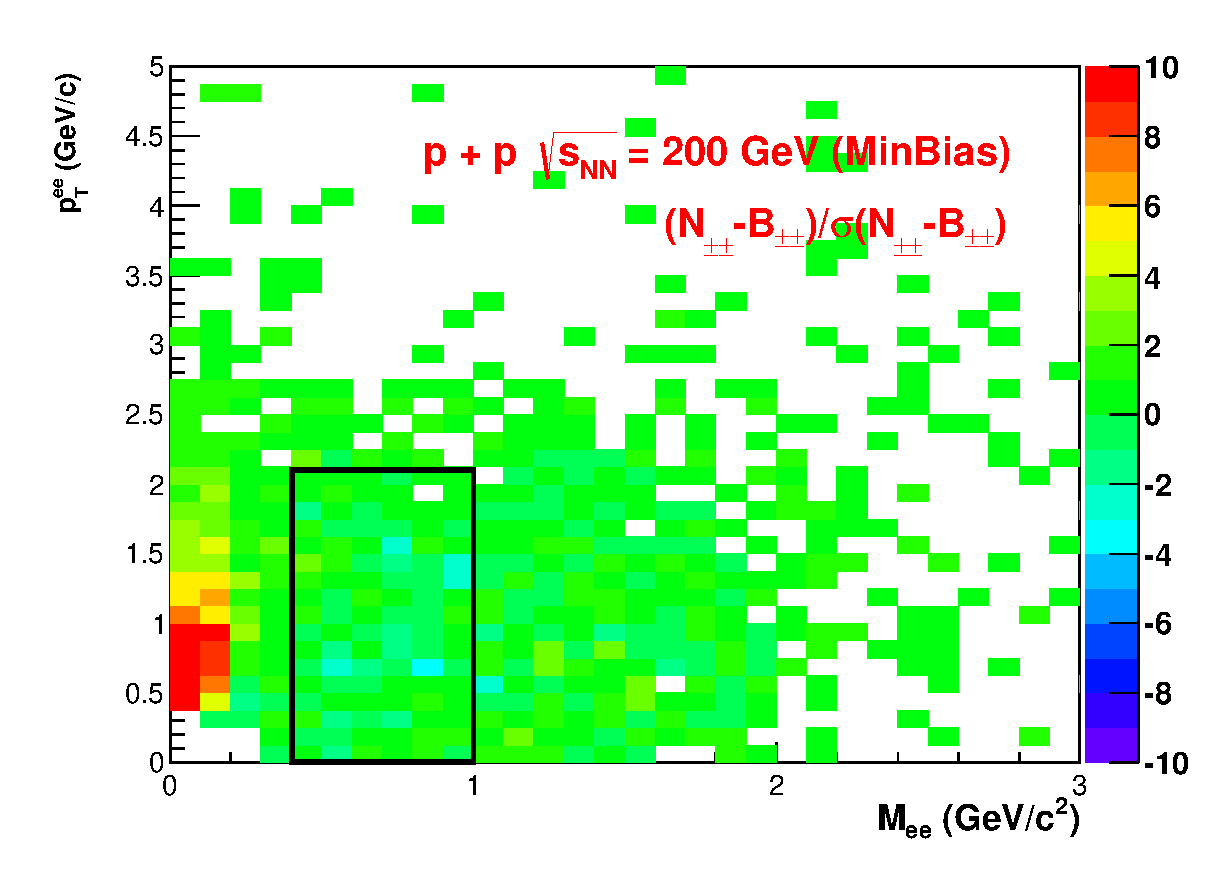
\includegraphics[width=0.45\textwidth]{fig/3.Analysis/background/pp/paper_nRegion}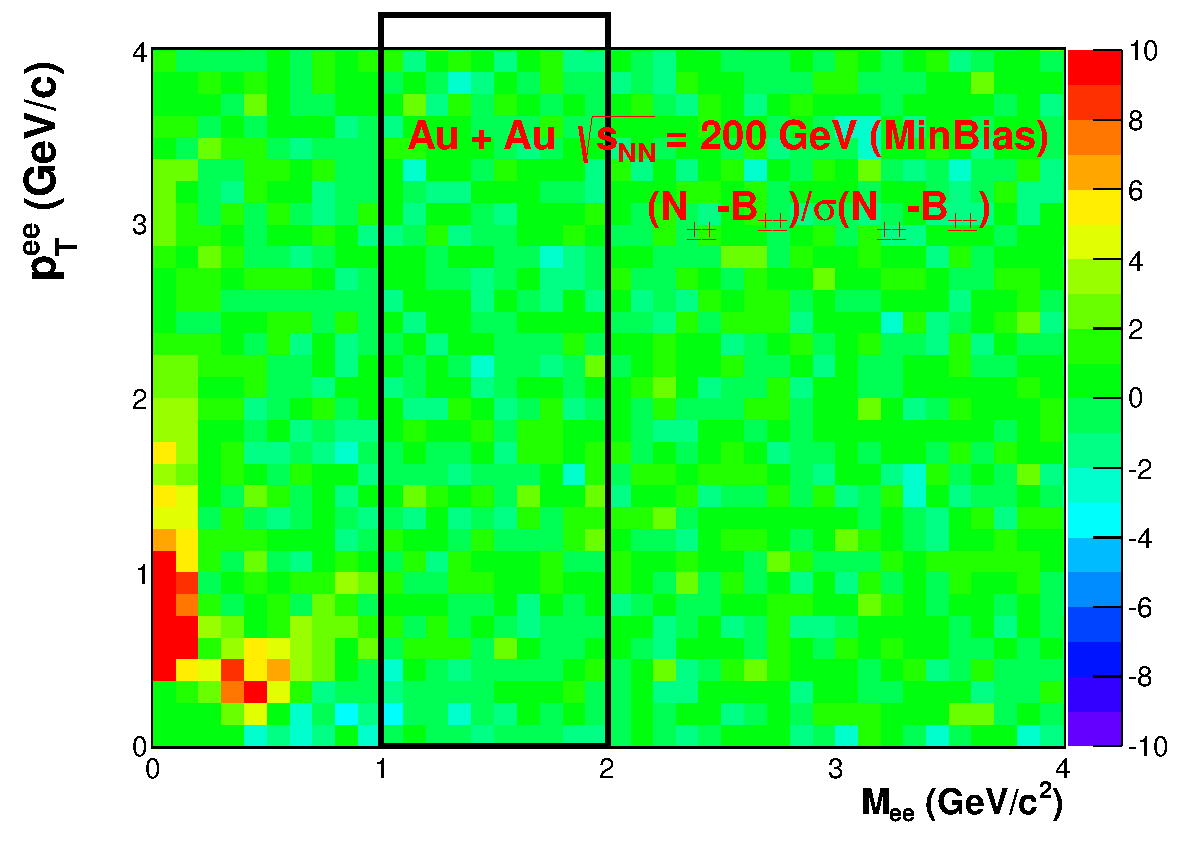
\includegraphics[width=0.45\textwidth]{fig/3.Analysis/background/AuAu/paper_nRegion}
\par\end{centering}

\protect\caption{The difference between like-sign background and mixed event background
divided by its standard deviation $(N_{likesign}-N_{likesign}^{Mix})/\sigma(N_{likesign}-N_{likesign}^{Mix})$
in p+p collision (left) and in Au+Au collision (right). the black
box represent the chosen normalization region: $0.5<M_{ee}<1GeV/c^{2}$,
$0<p_{T}^{ee}<2GeV/c$ for p+p data and $1<M_{ee}<2GeV/c^{2}$ for
Au+Au data.}


\label{fig:norRegion}
\end{figure}


\begin{figure}
\begin{centering}
\includegraphics[width=0.45\textwidth]{fig/3.Analysis/background/AuAu/paper_ratio}\includegraphics[width=0.45\textwidth]{fig/3.Analysis/background/pp/paper_ratio}
\par\end{centering}

\protect\caption{The distribution of like-sign over mixed event background ratio as
a function of $M_{ee}$. The solid line depicts a fit to the raise
about 1 $GeV/c^{2}$, while the dashed line shows 68\% confidence
level of the fit.}


\label{fig:LS/Mix}
\end{figure}



\subsection{Photon conversion}

Photon conversion is that photon hit material of detectors and convert
to $e^{+}e^{-}$ pairs. When reconstructed unlike-sign foreground,
it has contribution to the very low mass region ($M_{ee}<0.2GeV/c^{2}$).
Therefore, it must be subtracted from the signal. The pair mass from
photon conversion pairs should be 0. However, momentum of electron
tracks from conversion vertex away from primary vertex is biased which
lead to a finite pair invariant mass, because the procedure of reconstruction
primary tracks also included the primary vertex as a fit point. 

In this analysis, we used $\phi_{V}$ cut method which is similar
to the method used by PHENIX \cite{PhysRevC.81.034911}. Considering
the zero opening angle of di-electron pairs from photon conversion,
electron is bended inside the plate perpendicular to magnet direction.
Therefore, $\phi_{V}$ is defined as Eq. \ref{eq:phiV}, where $\vec{p}_{+}$,
$\vec{p}_{-}$ are the momentum of $e^{+}$ and $e^{-}$, respectively,
$\hat{z}$ is the direction of magnet.
\begin{align}
\hat{\mu} & =\frac{\vec{p}_{+}+\vec{p}_{-}}{|\vec{p}_{+}+\vec{p}_{-}|}\,,\:\hat{\nu}=\vec{p}_{+}\times\vec{p}_{-}\nonumber \\
\hat{\omega} & =\hat{\mu}\times\hat{\nu}\,,\:\hat{\omega}_{c}=\hat{\mu}\times\hat{z}\label{eq:phiV}\\
 & \cos\phi_{V}=\hat{\omega}\cdot\hat{\omega}_{c}\nonumber 
\end{align}
 

$\phi_{V}$ should be zero, if the di-electron pair is originated
from photon conversions. While, there is no preferred orientation
for combinatorial pairs, and very weak dependence for di-electron
pairs from hadron decays. A Geant simulation was done to study the
distribution of $\phi_{V}$ vs mass (Fig \ref{fig:phiV}(left) \cite{:fv}).
And the cut used in this analysis is shown as the red solid line.
The conversion pairs were directly removed by this cut. This cut was
only applied in very low mass ($M_{ee}<0.2GeV/c^{2}$). Simulation
shows \textasciitilde{}95\% conversion pairs are removed by this cut.

\begin{figure}
\begin{centering}
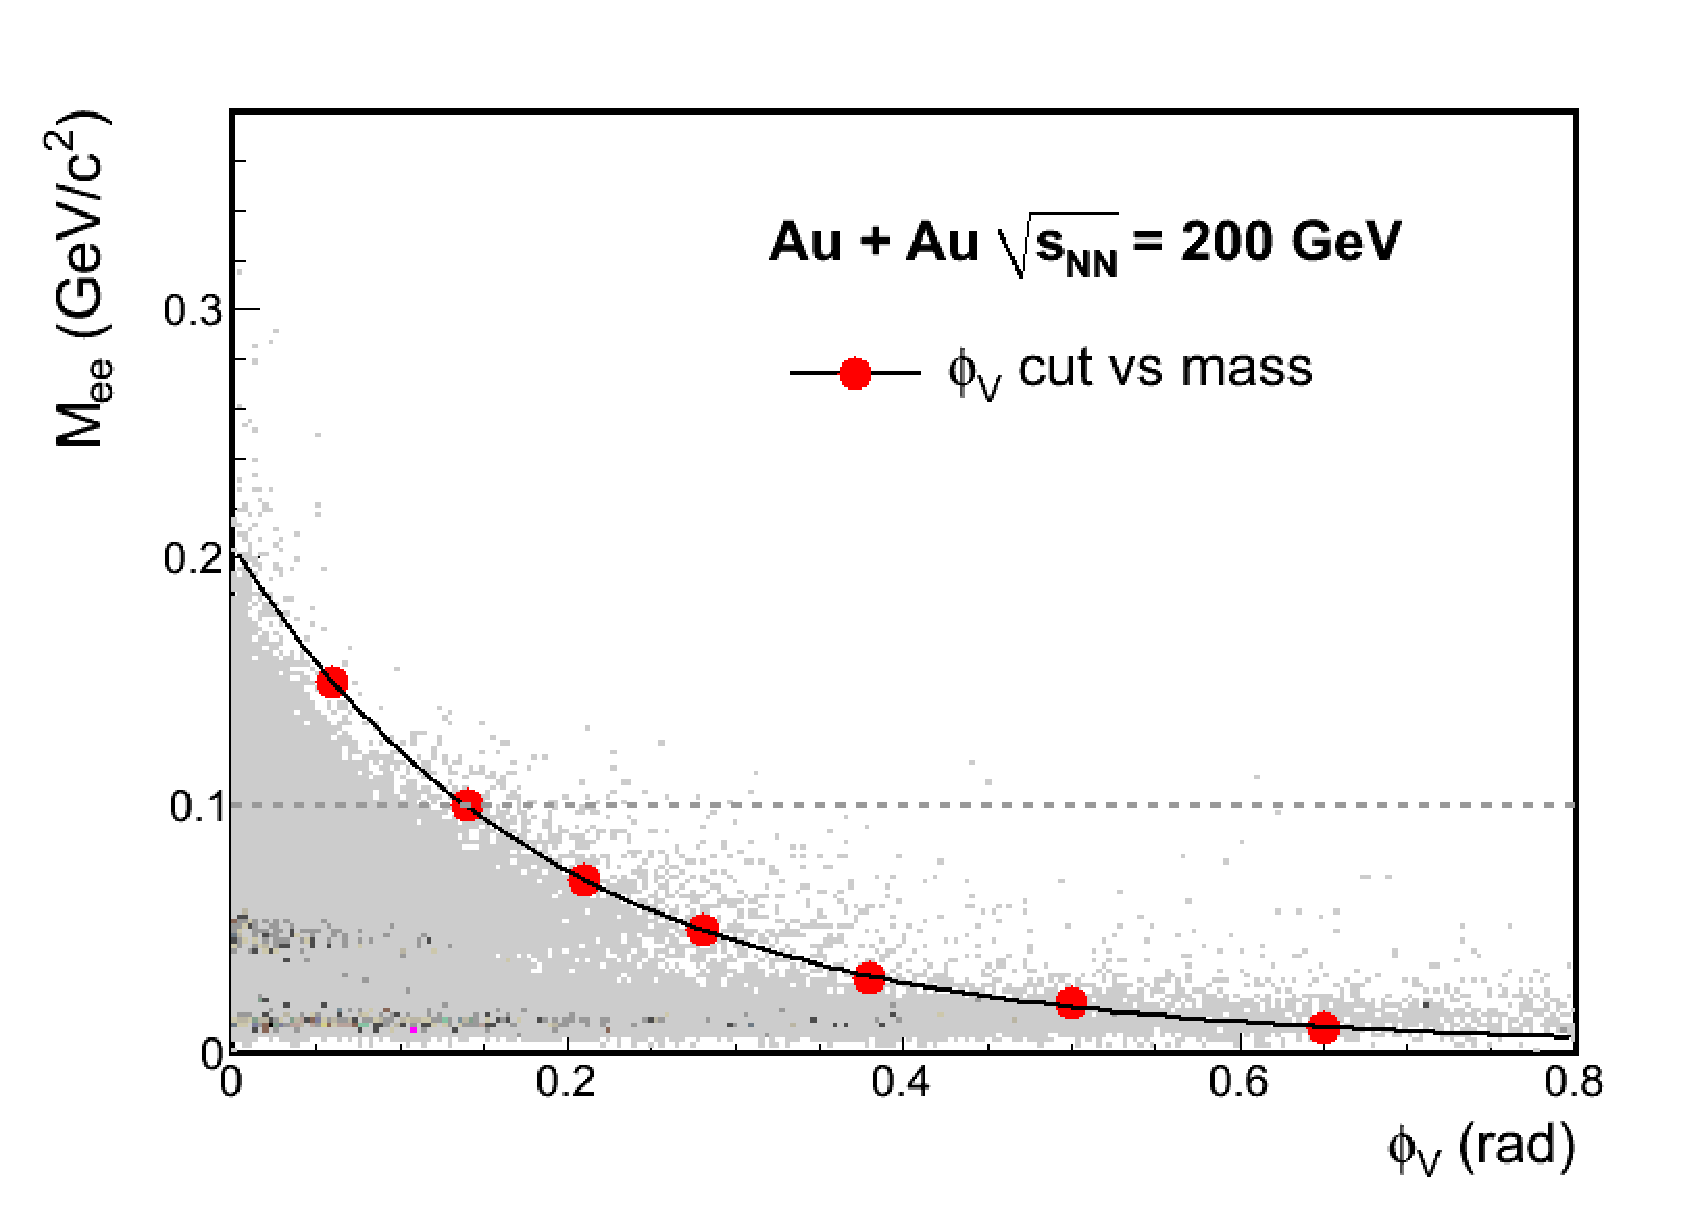
\includegraphics[width=0.45\textwidth]{fig/3.Analysis/Additional/pic_phiV}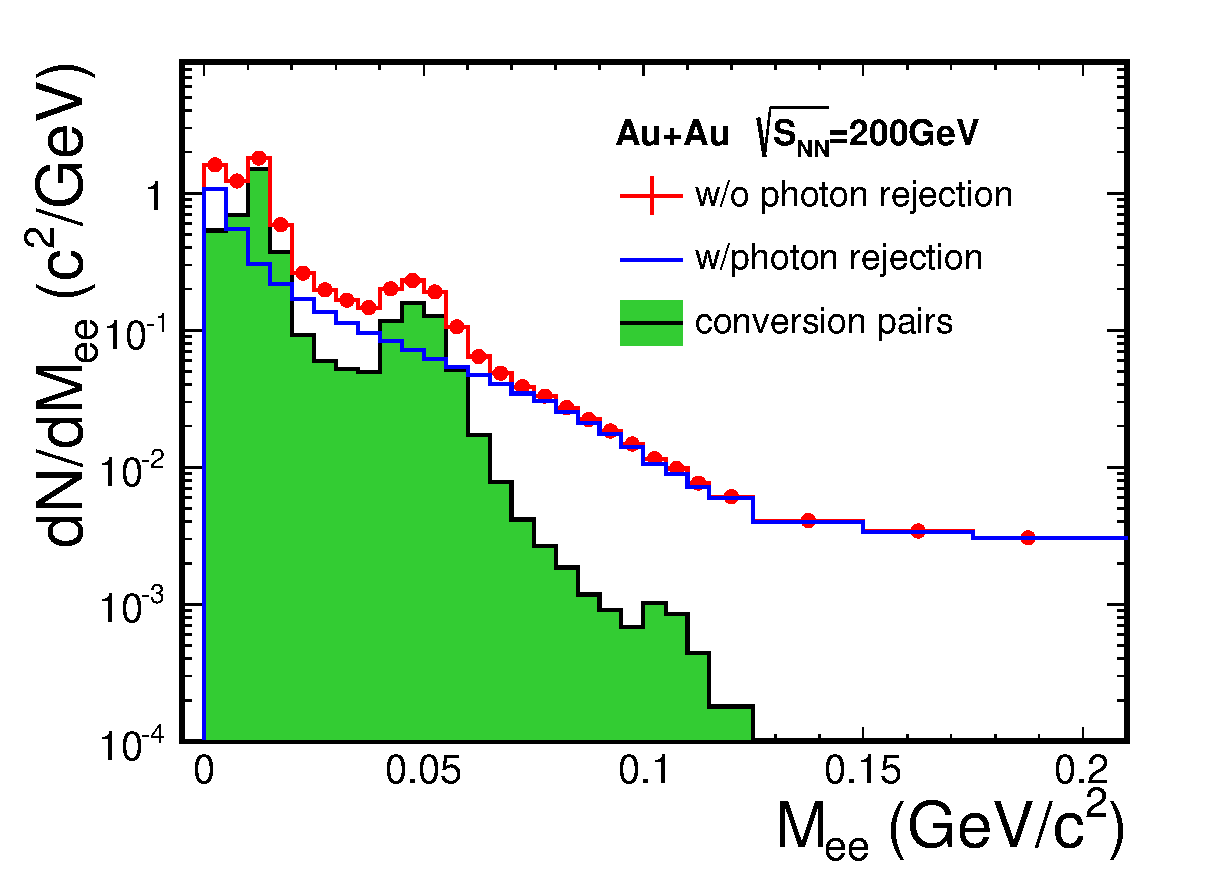
\includegraphics[width=0.45\textwidth]{fig/3.Analysis/Additional/conversion}
\par\end{centering}

\protect\caption{(left) $\phi_{V}$ \emph{vs mass} distribution from Geant simulation,
the solid line depicts the cut. (right) Di-electron mass spectra with
photon rejection, without photon rejection and conversion pairs distribution
from 200GeV Au+Au data. The conversion peaks from left to right are
came from conversion happened at beam pipe (r\textasciitilde{}4cm),
TPC supporting structure (r\textasciitilde{}20cm) and TPC inner field
cage (r\textasciitilde{}46cm) ,  respectively.}


\label{fig:phiV}
\end{figure}



\subsection{Centrality and $p_{T}^{ee}$ dependence}

In this analysis, for the Au+Au collision data, we also measured the
di-electron mass spectra in different centrality bins and $p_{T}^{ee}$
regions. The centrality and $p_{T}^{ee}$ dependence of acceptance
factor and correlated residue were also studied. Figure \ref{fig:acc pT cen}
shows the acceptance factor correction (acceptance difference between
unlike-sign pairs and like-sign pairs ) in different centrality and
$p_{T}$ bins. The acceptance factor shows a clear $p_{T}$ dependence.
It is because the bending effect in magnetic field is weaker for charged
particles with higher $p_{T}$ . The acceptance between positive and
negative charged tracks is smaller at higher $p_{T}$. The correlation
background residue distribution were also studied by using function
\ref{eq:LSresidue} to fit the like-sign over mixed event background
ratio in different centrality and $p_{T}$ regions (Fig \ref{fig:LMR cen pT}).

\begin{figure}
\begin{centering}
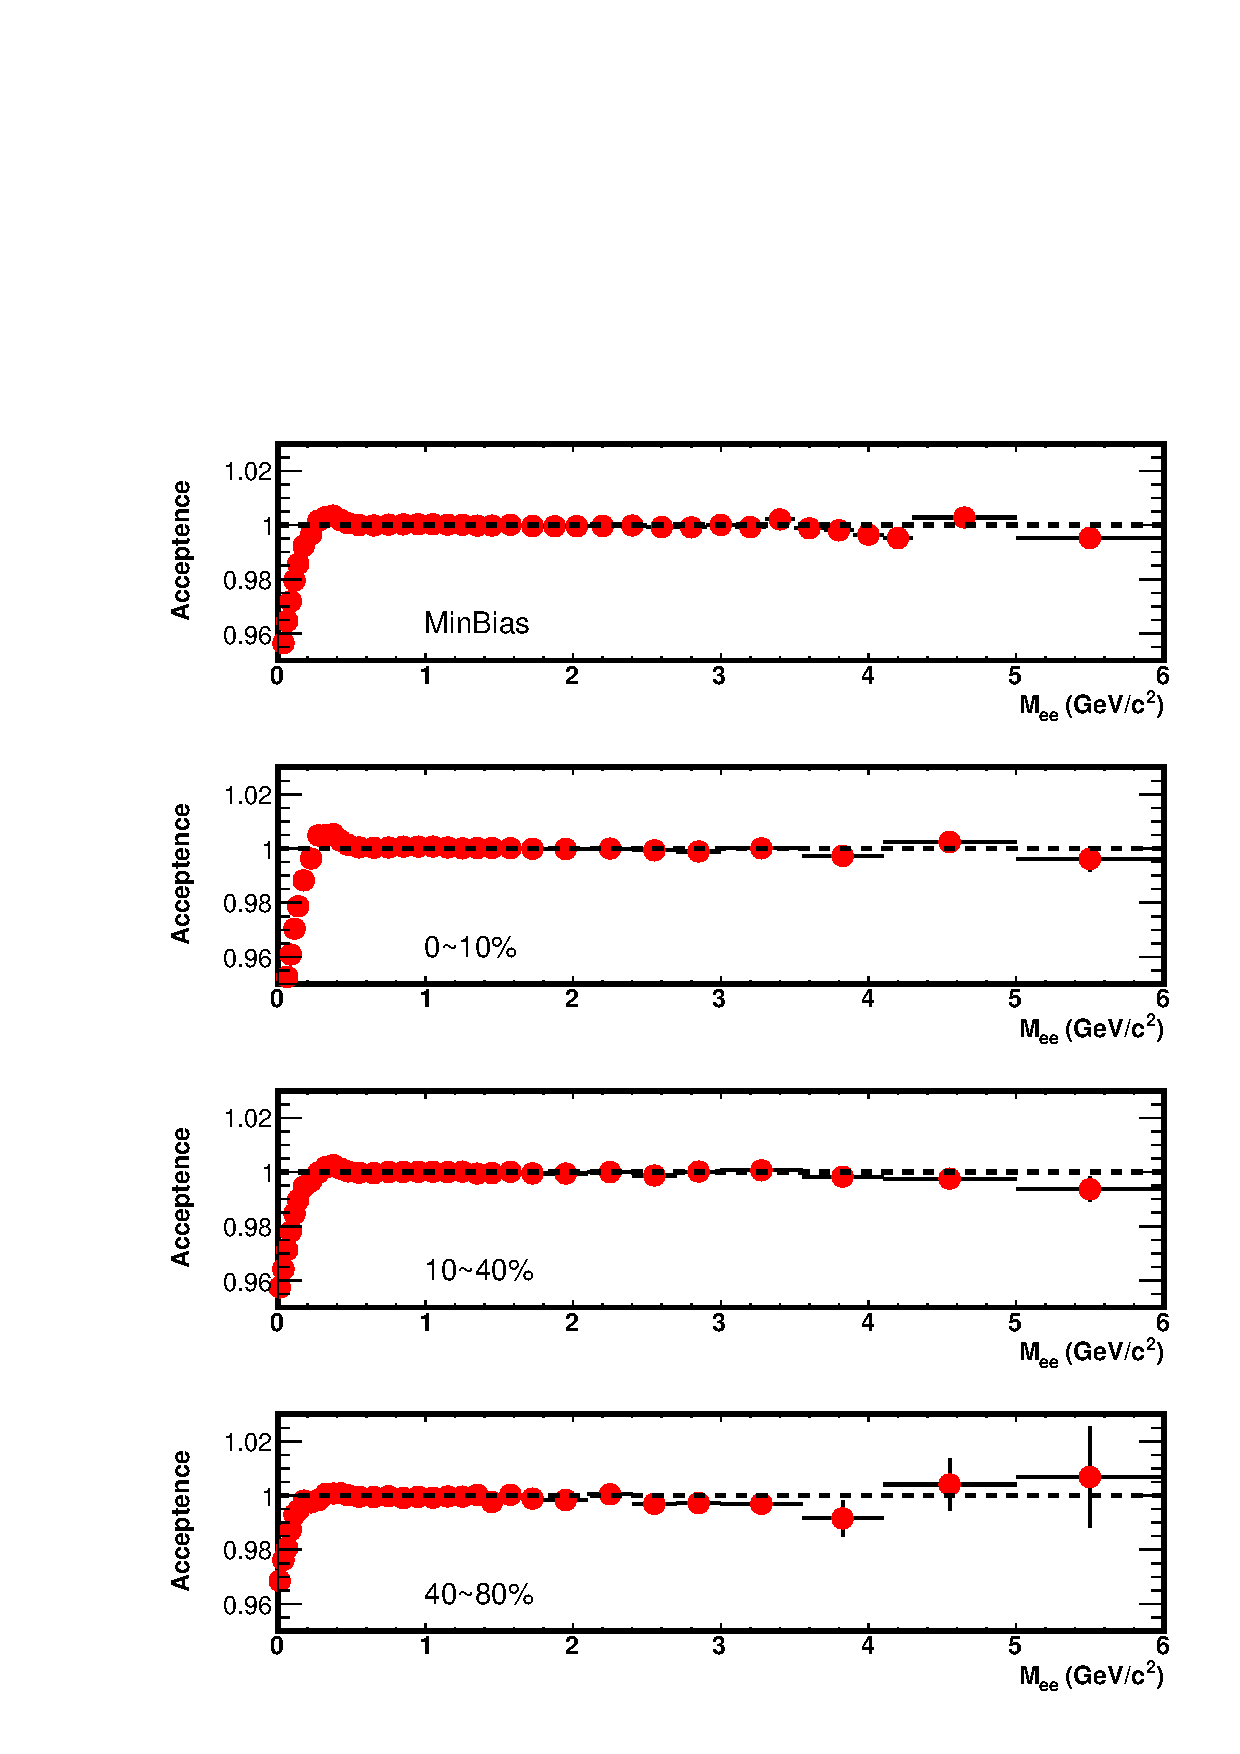
\includegraphics[width=0.45\textwidth]{fig/3.Analysis/Run11/Acc_cen}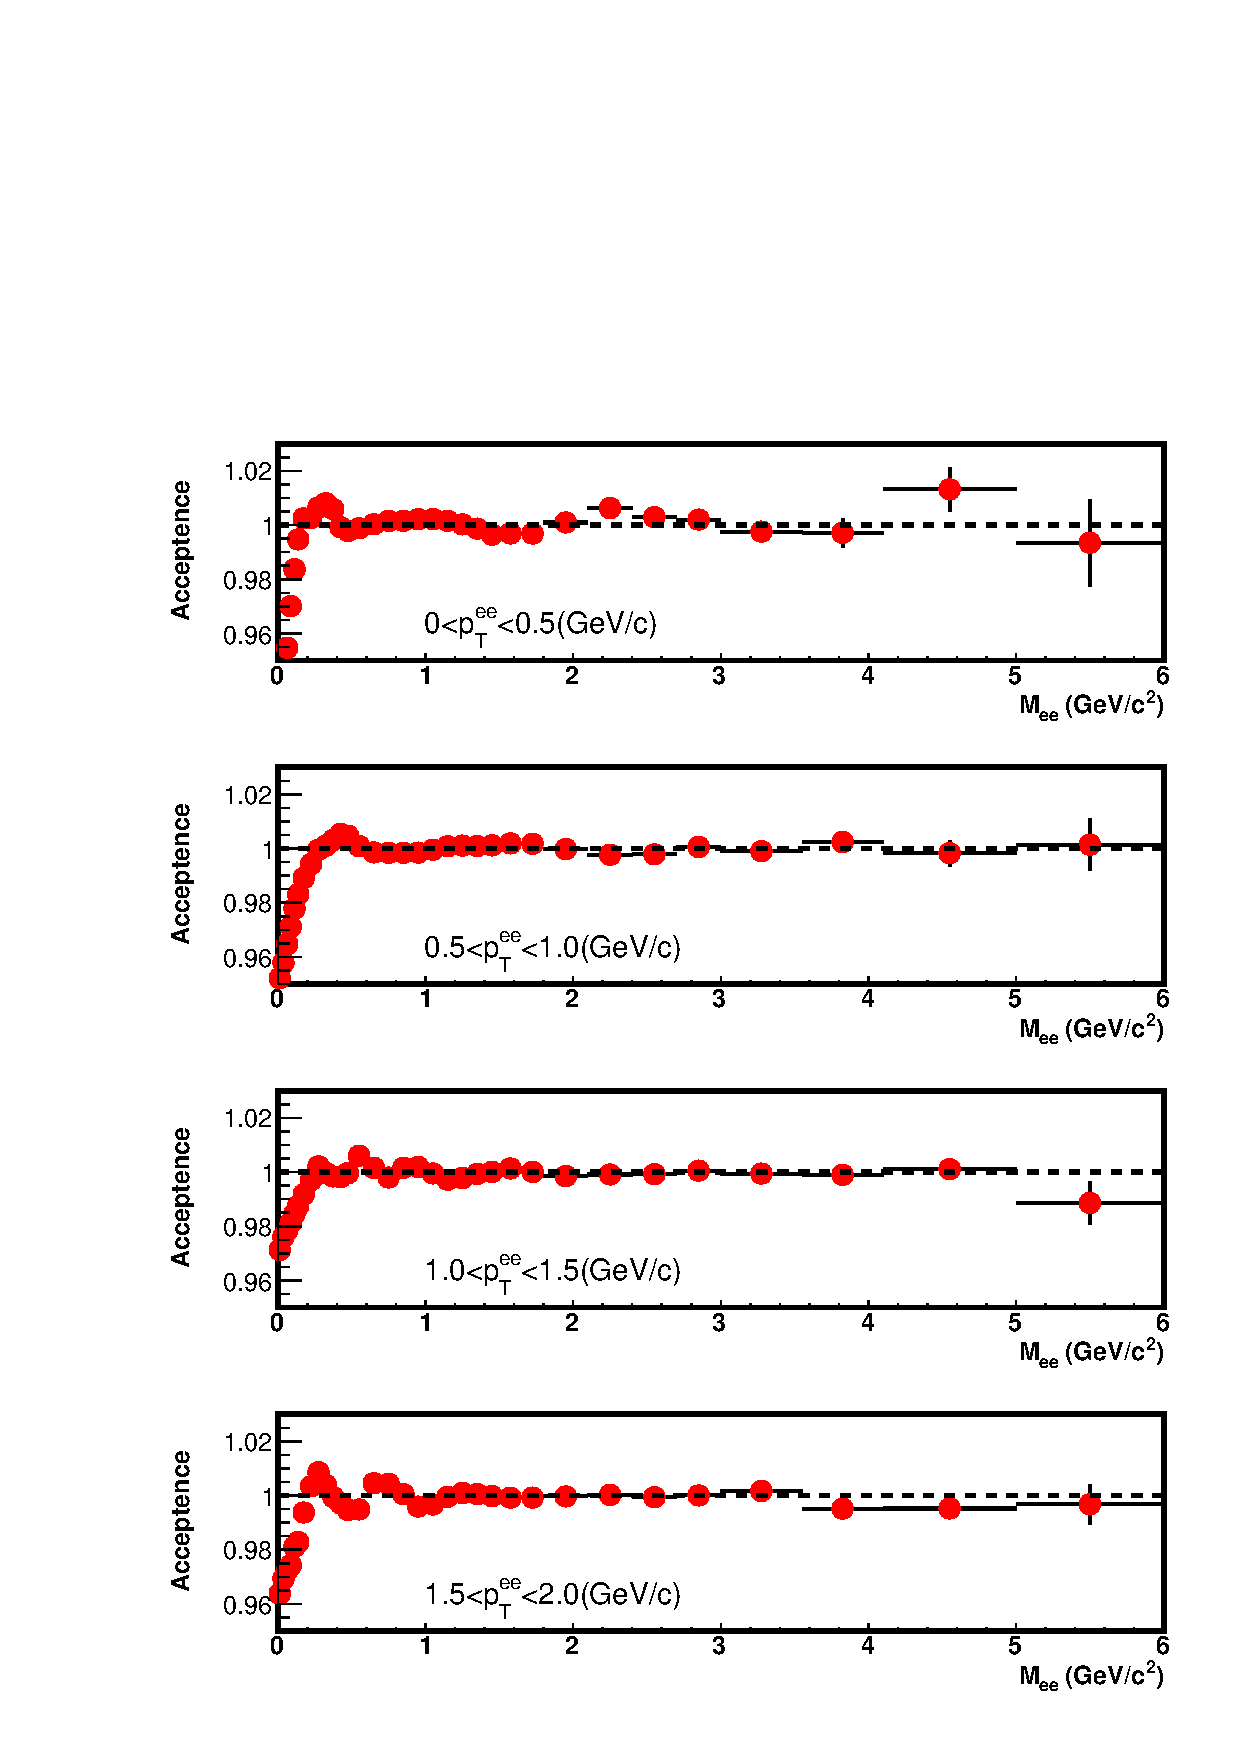
\includegraphics[width=0.45\textwidth]{fig/3.Analysis/Run11/Acc_pT}
\par\end{centering}

\protect\caption{Acceptance factor in different centrality (left) and $p_{T}$ (right)
bins, for 200 GeV Au+Au collision data.}


\label{fig:acc pT cen}
\end{figure}


\begin{figure}
\begin{centering}
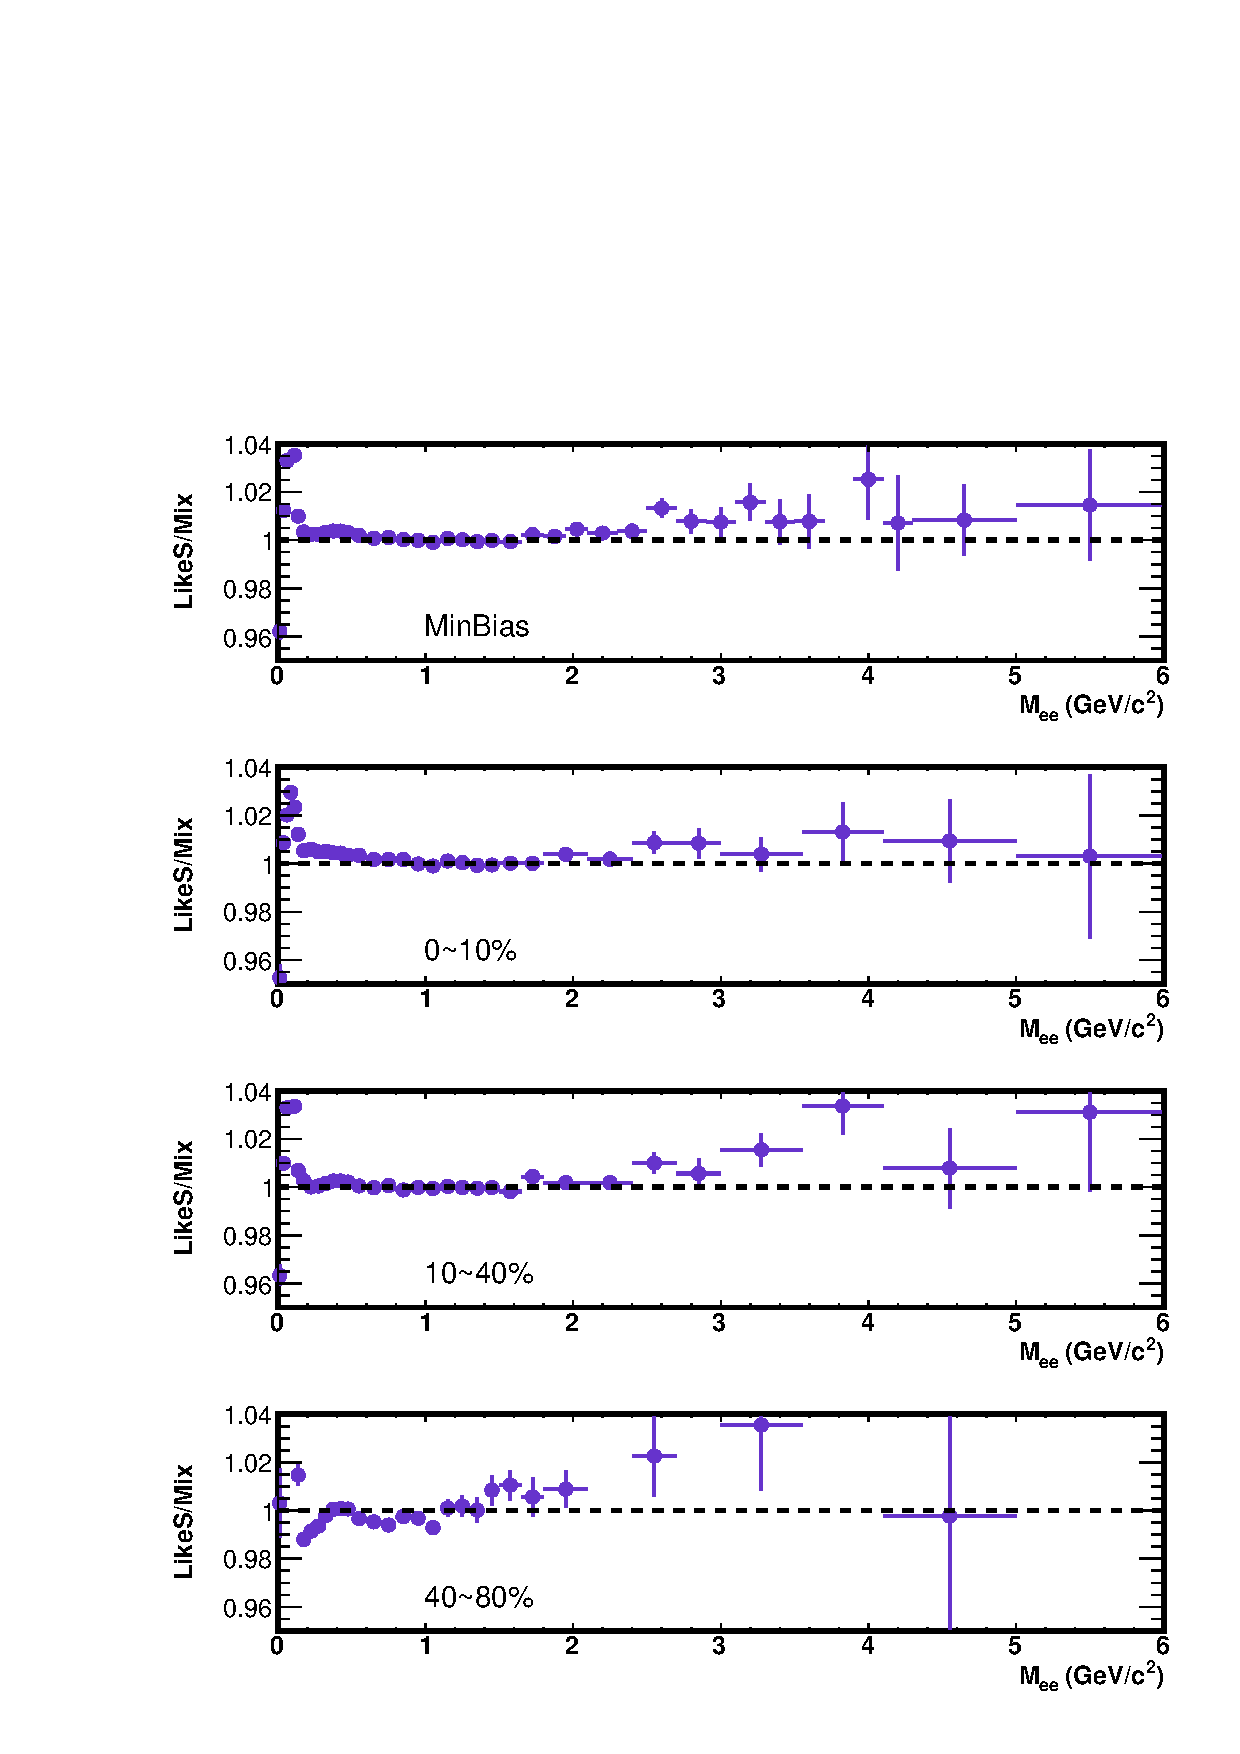
\includegraphics[width=0.45\textwidth]{fig/3.Analysis/Run11/LMR_cen}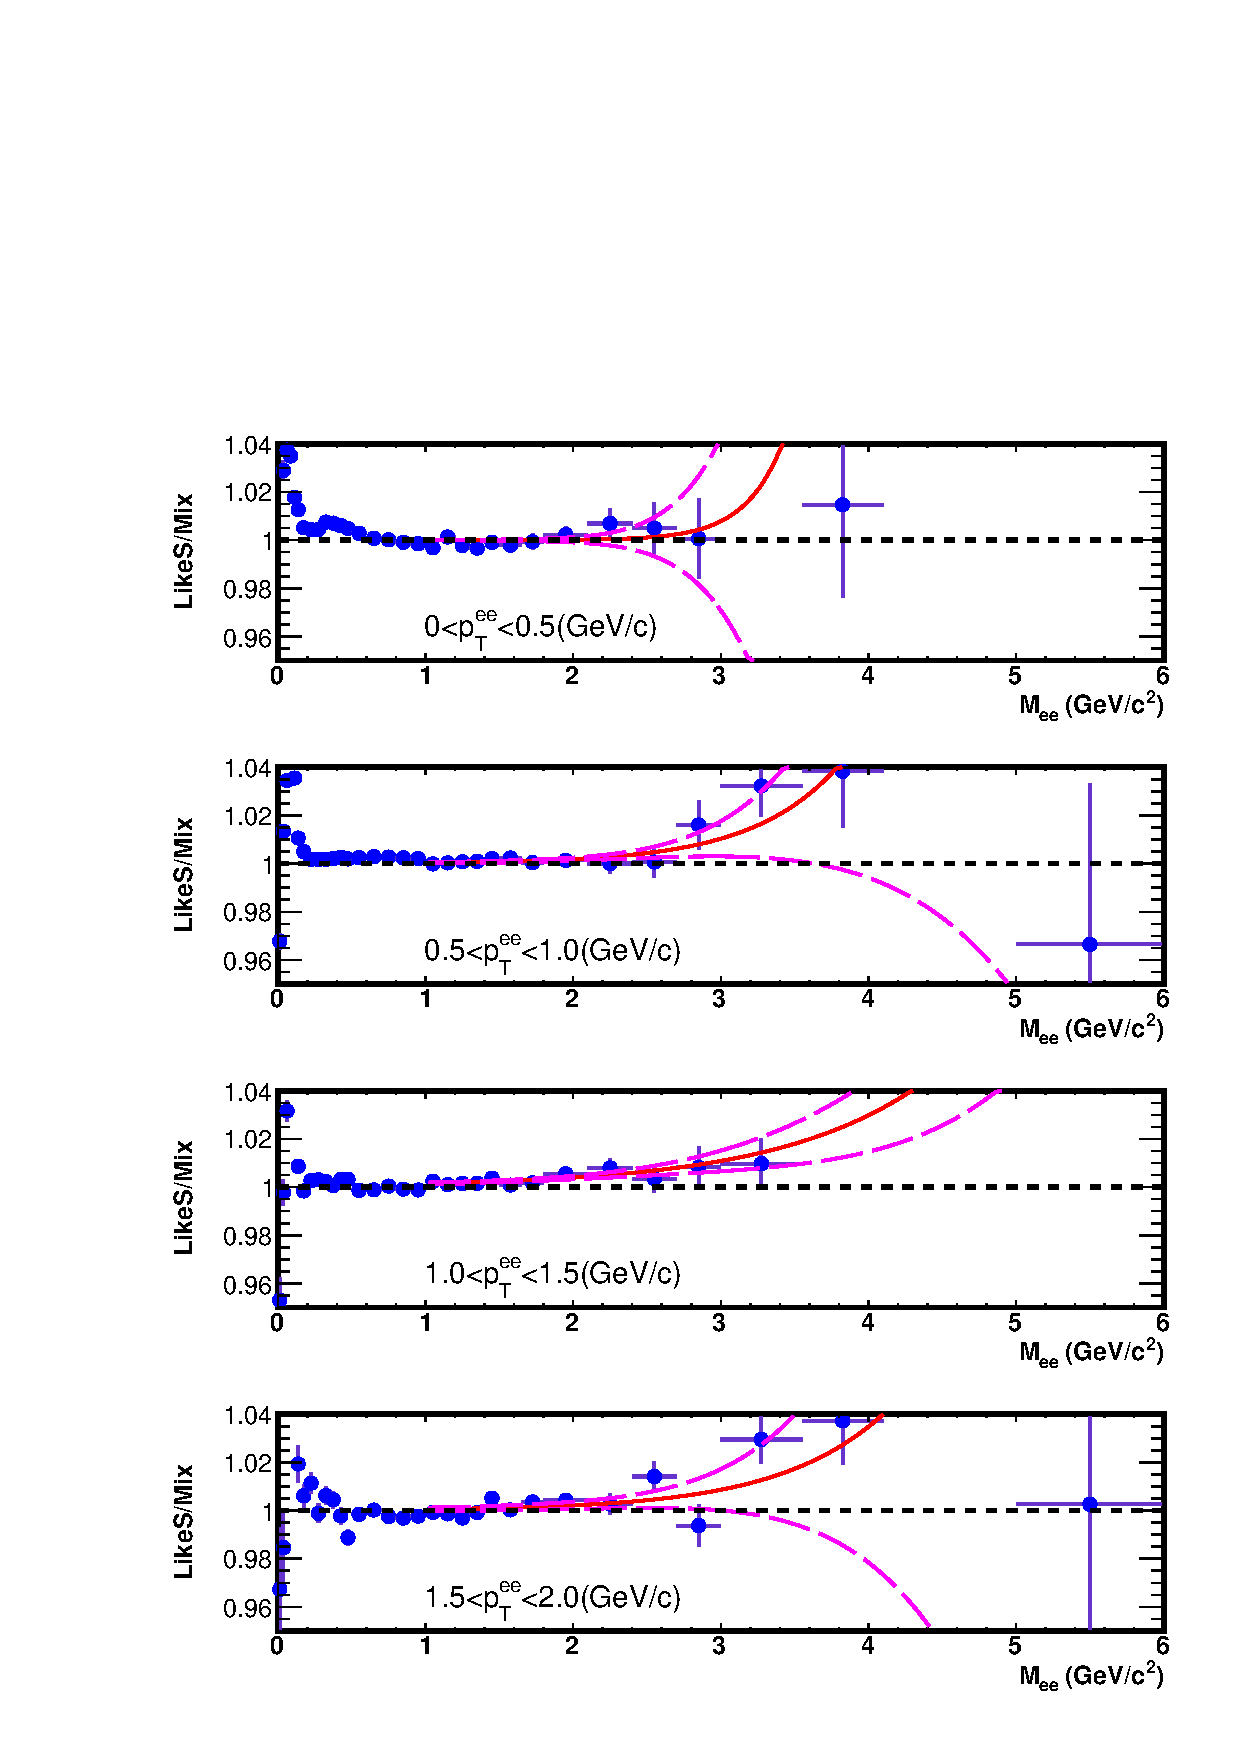
\includegraphics[width=0.45\textwidth]{fig/3.Analysis/Run11/LMR_pT}
\par\end{centering}

\protect\caption{Like-sign over mixed event background ratio in different centrality
(right) and $p_{T}$ (left) bins, for 200 GeV Au+Au collision data.}


\label{fig:LMR cen pT}
\end{figure}



\subsection{Di-electron signal}

The follow tactics was used to subtract the background from the unlike-sign
foregound:
\begin{itemize}
\item Considering the correlated component, we subtracted the like-sign
background with a acceptance factor correction in mass region ($M_{ee}<M_{th}$,
where $M_{th}=1GeV/c^{2}$ for Au+Au collision, and $M_{th}=0.4GeV/c^{2}$
for p+p collision), where the like-sign background has enough statistics.
\item For the mass region above $M_{th}$, the normalized mixed event background
was subtracted. And we subtracted the correlated component (Jet contribution)
by fitting the ratio of like-sign over mixed event background (Eq.
\ref{eq:LSresidue}).
\end{itemize}
After the background subtraction, we got the raw di-electron spectra
without efficiency correction. Figure \ref{fig:RYandSBratio} shows
di-electron signal, foreground and background, as well as the signal
over background ratio.
\begin{lyxcode}
\begin{figure}
\begin{centering}
\begin{minipage}[t][1\totalheight][s]{0.33\columnwidth}%
\begin{center}
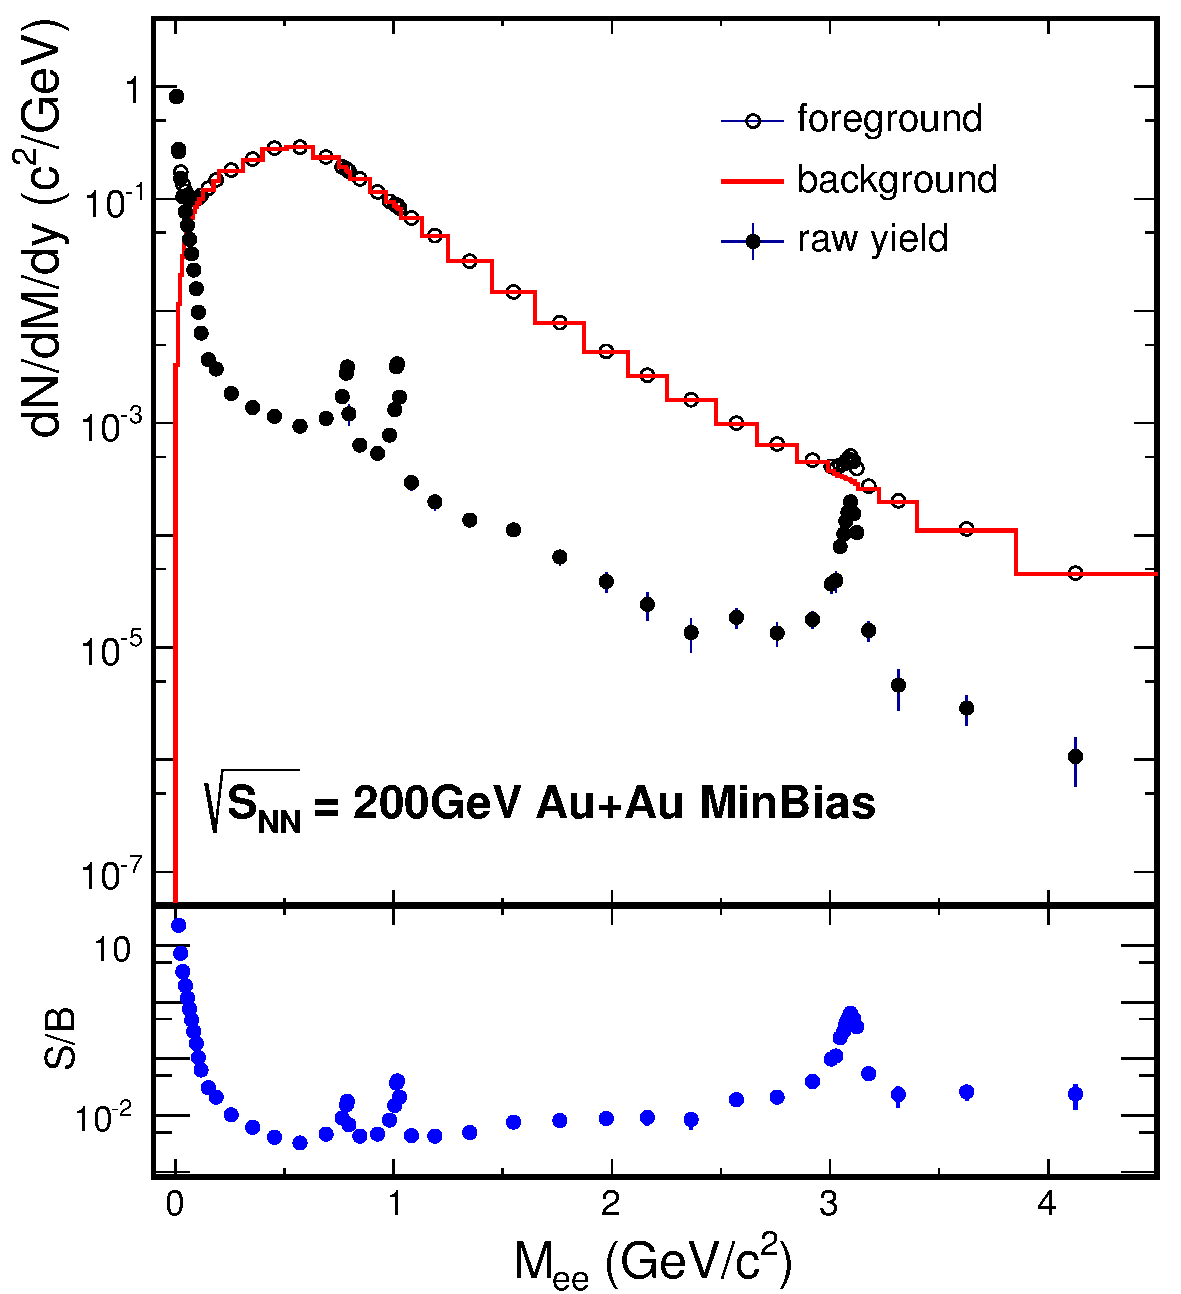
\includegraphics[width=1\textwidth]{fig/3.Analysis/background/AuAu/SBRatio_AuAu_MinBias}
\par\end{center}%
\end{minipage}%
\begin{minipage}[t][1\totalheight][s]{0.33\columnwidth}%
\begin{center}
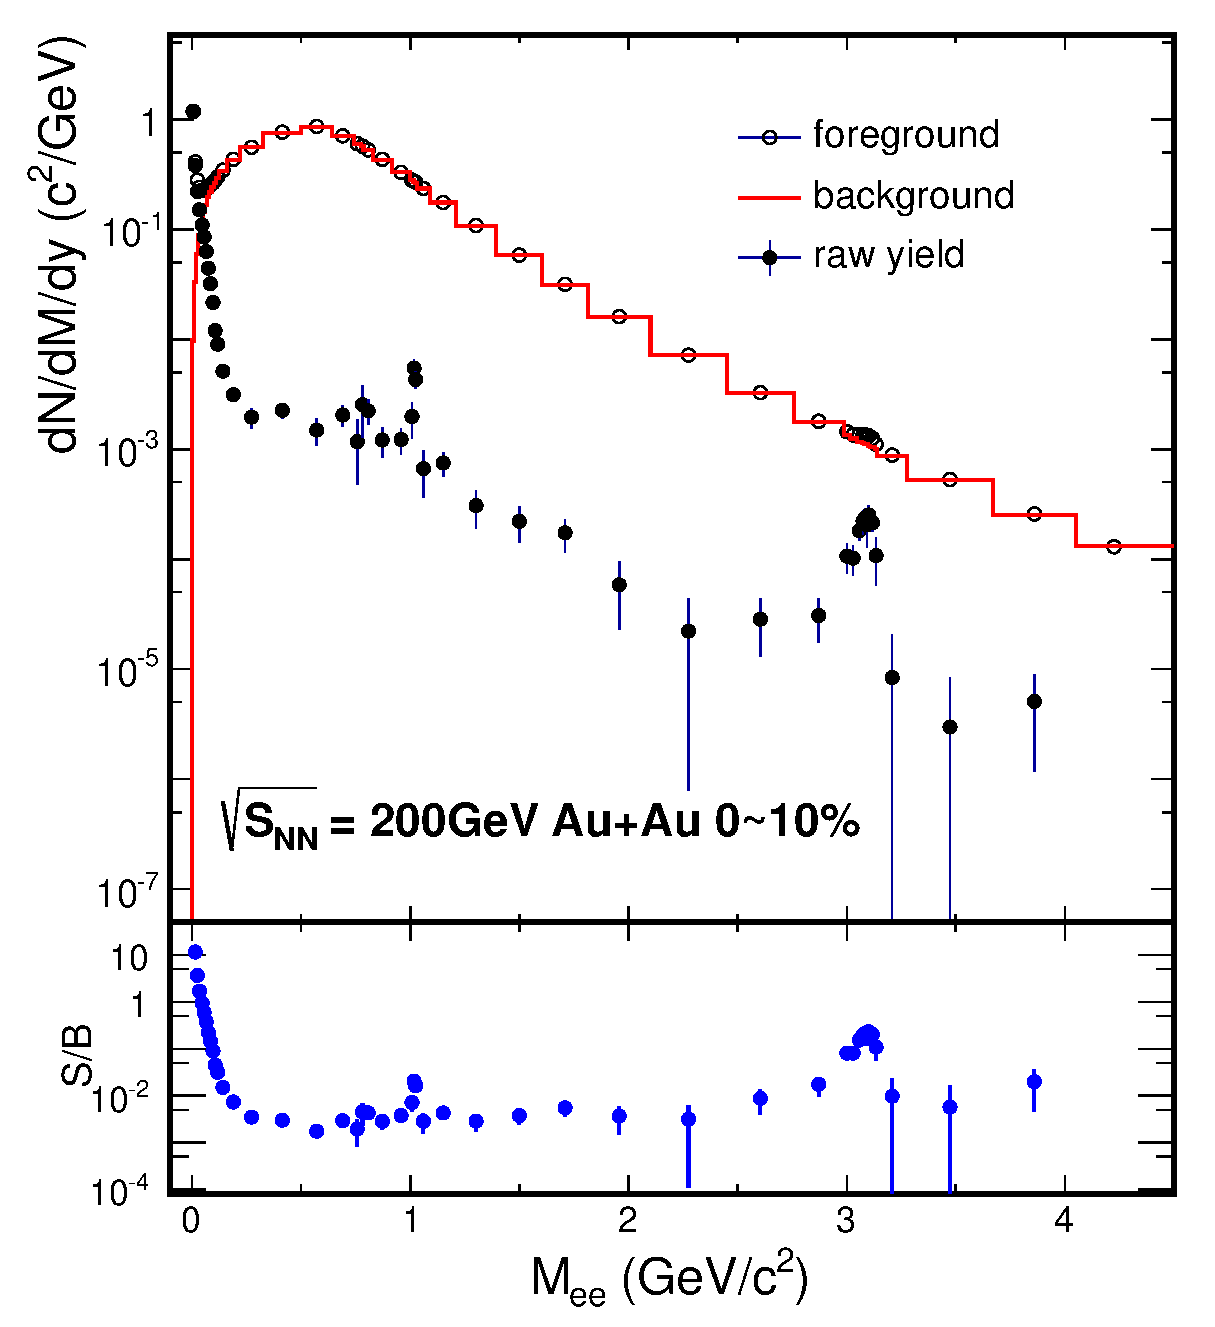
\includegraphics[width=1\textwidth]{fig/3.Analysis/background/AuAu/SBRatio_AuAu_Cen}
\par\end{center}%
\end{minipage}%
\begin{minipage}[t][1\totalheight][s]{0.33\columnwidth}%
\begin{center}
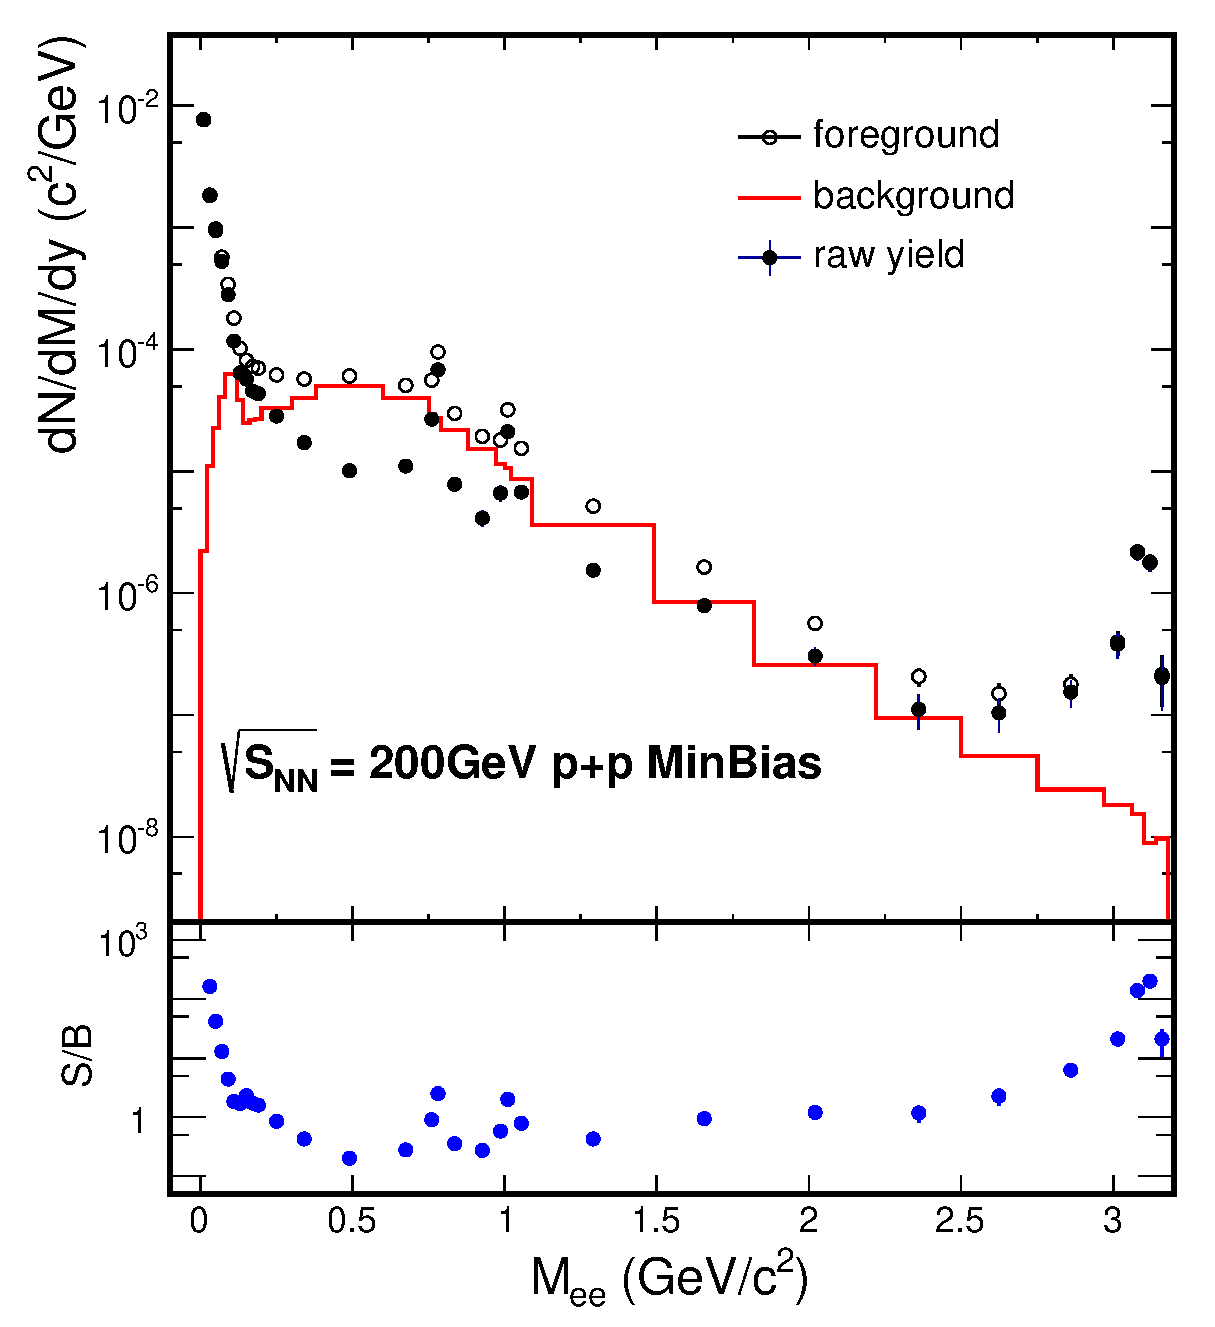
\includegraphics[width=1\textwidth]{fig/3.Analysis/background/pp/SBRatio_PP_MinBias}
\par\end{center}%
\end{minipage}
\par\end{centering}

\protect\caption{Unlike-sign foreground, background, raw di-electron spectra and signal
over background ratio for Au+Au minimum bias (left), central (middle)
collision and p+p minimum bias (collision). }


\label{fig:RYandSBratio}
\end{figure}

\end{lyxcode}

\section{Efficiency and acceptance correction}

The di-electron raw signal yields was corrected for efficiency within
STAR acceptance of $|y_{ee}|<1$, $|\eta_{e}|<1$ and $p_{T}^{e}<0.2GeV/c$.
To calculate the efficiency, we first need single electron efficiency
which can be separated into two parts: detector efficiency and PID
efficiency. Then Monte Carlo method is used to evolved the single
efficiency into pair efficiency. We will discuss it step by step,
in the following sections.


\subsection{Single electron efficiency}

The single electron efficiency in this analysis included the TPC tracking
efficiency ($\varepsilon_{TPC}$), TOF matching efficiency ($\varepsilon_{TOF}$)
and electron identification efficiency ($\varepsilon_{PID}$) as Eq.
\ref{eq:single eff}.

\begin{equation}
\varepsilon_{single}=\varepsilon_{TPC}\times\varepsilon_{TOF}\times\varepsilon_{PID}\label{eq:single eff}
\end{equation}



\paragraph{TPC tracking efficiency}

The TPC tracking efficiency includes the track reconstruction efficiency
and the TPC acceptance loss. Also the track quality cut (nHitFits,
dca) efficiency are also combined into TPC tracking efficiency. The
TPC tracking efficiency was obtained via the standard STAR embedding
process. Monte Carlo (MC) electron tracks were generated within a
certain phase space definition. The embedding tracks were sent into
the GSTAR simulator and passed through STAR detector geometry corresponding
to the data set and detector response simulator (TRS, TPC Response
Simulator) to simulate the detector signal. Then, the MC tracks were
mixed with the real data which we called embedding sample here. The
embedding sample were reconstructed by the same offline reconstruction
chain used to produce real data. The tracking efficiency is defined
by number of reconstructed MC tracks which is satisfied the track
quality cut divided by number of input MC tracks, also see Eq. \ref{eq:effTPC}.

\begin{equation}
\varepsilon_{TPC}=\frac{N_{rc}(nHitsFit\geqslant20,\, dca<1cm)}{N_{Mc}}\label{eq:effTPC}
\end{equation}


To qualify whether the embedding sample can reproduce the real data,
we compared several track parameters (\emph{nHitsFit, dca}) from embedding
sample with those from the pure electron sample selected by photon
conversion and $\pi^{0}$ Daliza decay. The difference was included
into the systematic uncertainty.


\paragraph{TOF efficiency}

The TOF efficiency ($\varepsilon_{TOF}$) was studied via comparing
the number of track which matches TOF and the total number of TPC
primary tracks from real data. A track match to TOF was defined as
following:
\begin{itemize}
\item The track is projected to the radius of TOF, and there is a valid
hit in the corresponding TOF cell (tofMatchFlag>0 in data structure).
\item The distance between the projection position to the TOF cell center
in y coordinate (Localy) is smaller than 1.8 cm.
\end{itemize}
The definition of TOF matching efficiency is also shown as Eq. \ref{eq:eff TOF}.

\begin{equation}
\varepsilon_{TOF}=\frac{N_{matched}(tofMatchFlag>0\,\&\&\,|LocalY|<1.8cm)}{N_{TPC}}\label{eq:eff TOF}
\end{equation}


To achieve enough statistics to study the efficiency in 3 dimensions
($p_{T}$, $\eta$, $\phi$), we used pure pion sample selected by
a very tight \emph{dE/dx }cut ($|n\sigma_{\pi}|<0.5$)$ $ to study
the $\eta$ and $\phi$ dependence. The TOF matching efficiency from
pure electron sample from photon conversion and $\pi^{0}$ Dalitz
decay was served as a standard. A weight on $\eta$ and $\phi$ dimensions
was applied to the electron sample to address the difference in $\eta$
and $\phi$ distribution with $\pi$ sample. The efficiency from $\pi$
sample was scaled to match with the one from electron sample. In this
analysis, we used following function to parameterize the scale factor
as a function of $p_{T}$ :

\begin{equation}
f(x)=\frac{1+ax+bx^{2}}{c+\exp\{(x-d)/f\}}\label{eq:eff tof diff}
\end{equation}
The fit result is shown in figure \ref{fig: TOF diff} and the difference
was also included in to the systematic uncertainty.

\begin{figure}
\begin{centering}
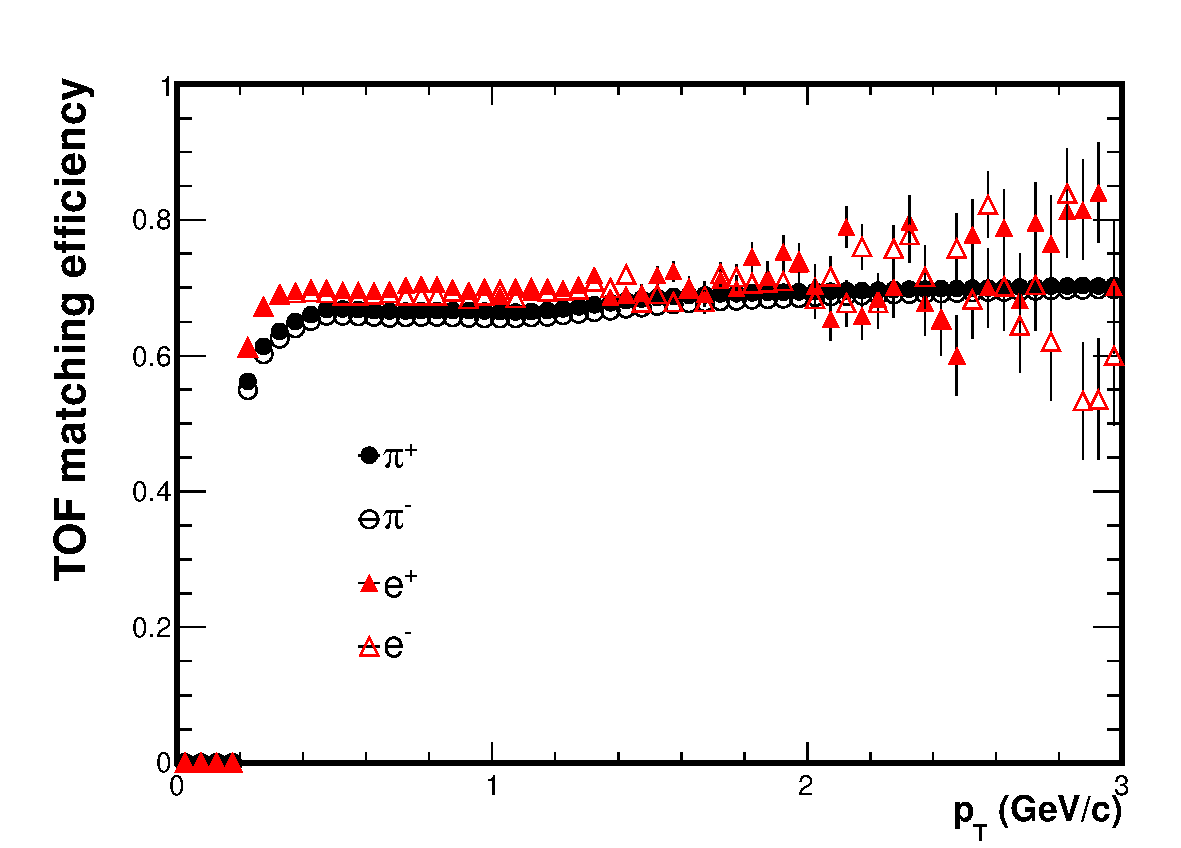
\includegraphics[width=0.45\textwidth]{fig/3.Analysis/Efficiency/TOF/Diff_phe_pi_rff}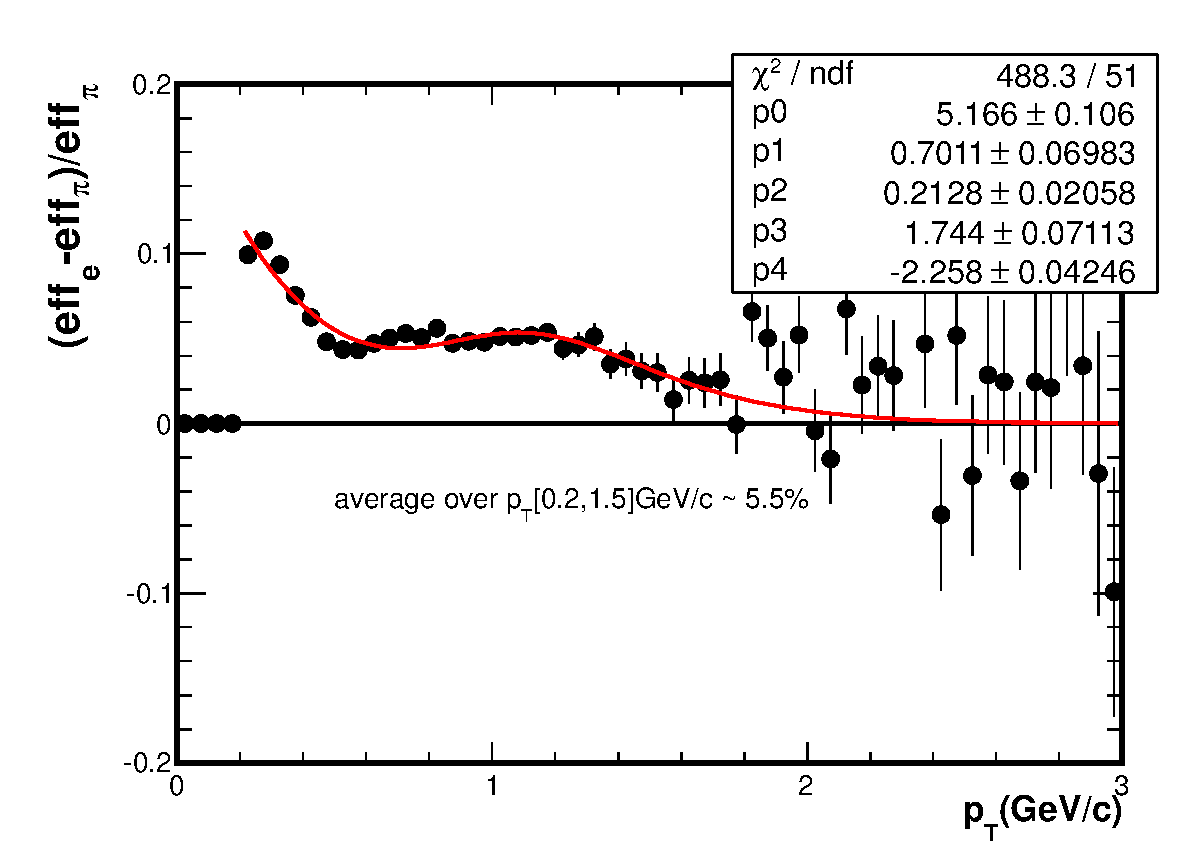
\includegraphics[width=0.45\textwidth]{fig/3.Analysis/Efficiency/TOF/SysErr_Tof}
\par\end{centering}

\protect\caption{(Left) TOF matching efficiency from $\pi$ sample and photon conversion
sample in Au+Au 200GeV minimum bias collision. They difference is
shown in the right panel. The red line depicts a fit by function \ref{eq:eff tof diff}.}


\label{fig: TOF diff}
\end{figure}


The TPC efficiency and TOF matching efficiency were both studied and
applied in 3 dimensions. TPC efficiency was calculated in $20\times36$
$\eta$, $\phi$ bins and 50 MeV $p_{T}$ bin, while TOF matching
efficiency was studied in $20\times60$ $\eta$, $\phi$ bins and
50 MeV $p_{T}$ bin. The centrality dependence was also taken into
account for Au+Au collision by comparing the $p_{T}$ distribution
from different centrality with minimum bias.


\paragraph{PID efficiency}

The PID efficiency included efficiency loss from $1/\beta$, $n\sigma_{e}$
and \emph{ndEdxFits }cut. $1/\beta$ cut and \emph{ndEdxFits} efficiency
was studied by the pure $\pi$ sample and the pure electron sample
from real data, their difference was considered as systematics uncertainty.
The pure electron sample was also used to study the $n\sigma_{e}$
distribution for electrons as mention in section 3.3.3 which provided
us the $n\sigma_{e}$ cut efficiency directly from the fit result. 

Figure \ref{fig:single eff AuAu} and \ref{fig:single eff pp} are
summary of the single tracking efficiency for Au+Au and p+p data sample.

\begin{figure}
\begin{centering}
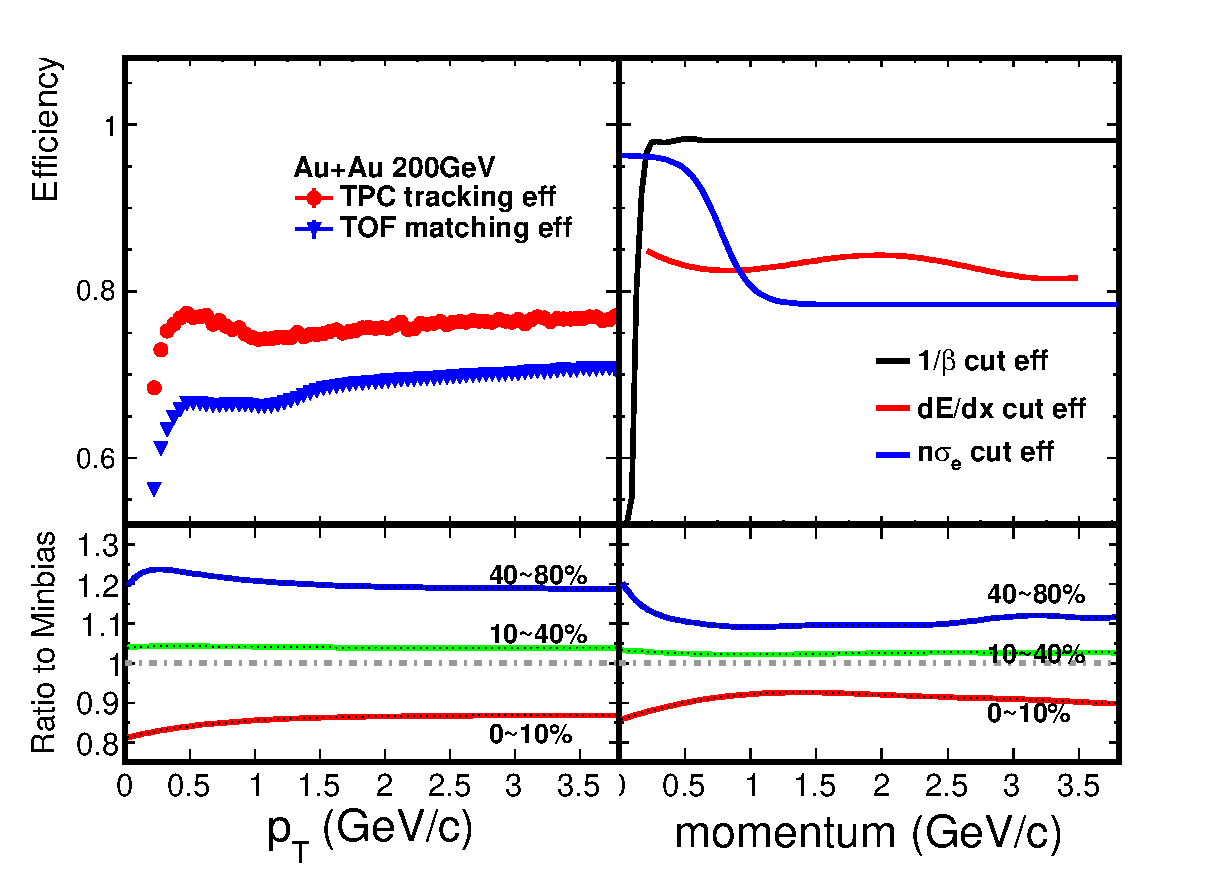
\includegraphics[width=0.8\textwidth]{fig/3.Analysis/Efficiency/single_eff_AuAu}
\par\end{centering}

\protect\caption{Summary of the single track efficiency for Au+Au 200 GeV.}


\label{fig:single eff AuAu}
\end{figure}


\begin{figure}
\begin{centering}
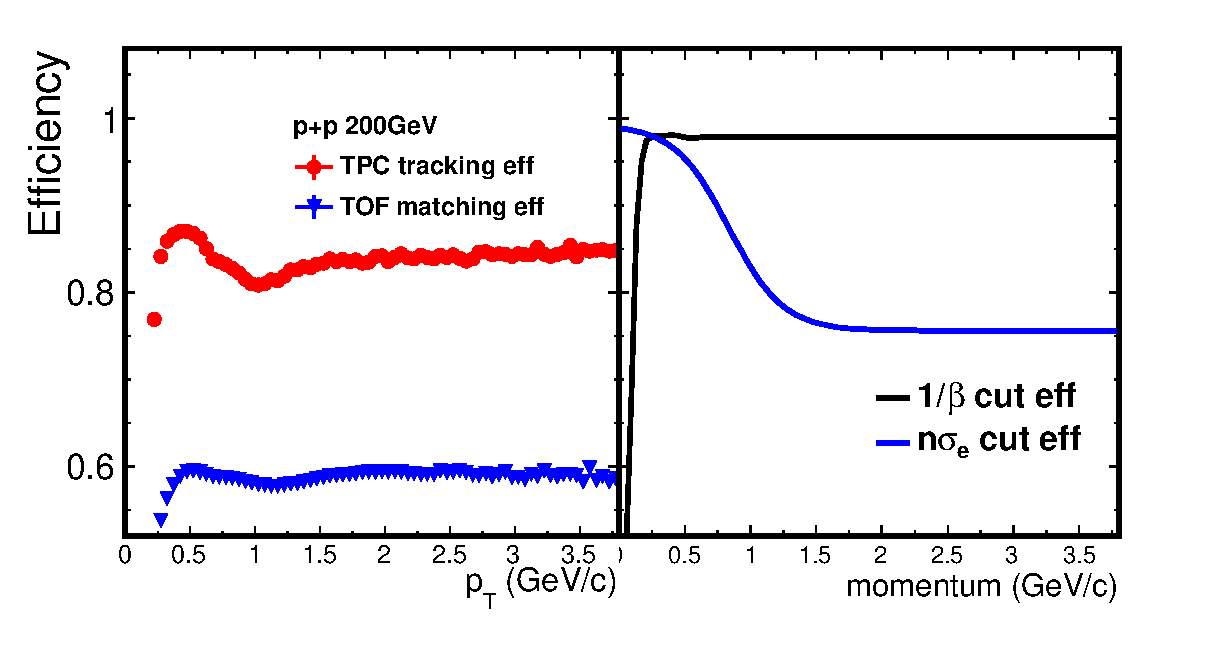
\includegraphics[width=0.8\textwidth]{fig/3.Analysis/Efficiency/single_eff_pp}
\par\end{centering}

\protect\caption{Summary of single track efficiency for p+p 200GeV.}


\label{fig:single eff pp}
\end{figure}



\subsection{Momentum resolution}

The momentum resolution for TPC tracks was studied by embedding sample
with the full detector simulation. Figure \ref{fig:mom Res} shows
the reconstructed electron $p_{T}^{rec}$ probability distribution
at a given input $p_{T}^{MC}$ from embedding sample for Au+Au 200
GeV collision. The distribution was parametrized with a double Crystal-Ball
function, defined in Eq. \ref{eq:mom res}:

\begin{equation}
P(p_{T}^{rec},\, p_{T}^{MC})\propto\begin{cases}
A\times(B-R)^{-n}, & R<-\alpha\\
e^{-R^{2}/2}, & -\alpha<R<\beta\\
C\times(D+R)^{-m}, & R>\beta
\end{cases}\label{eq:mom res}
\end{equation}


and 

\begin{align}
A & =(\frac{n}{|\alpha|})^{n}\times e^{-\alpha^{2}/2}\nonumber \\
B & =\frac{n}{|\alpha|}-|\alpha|\nonumber \\
C & =(\frac{m}{|\beta|})^{m}\times e^{-\beta^{2}/2}\label{eq: mom res2}\\
D & =\frac{m}{|\beta|}-|\beta|\nonumber \\
R & =(\frac{p_{T}^{rec}-p_{T}^{MC}}{p_{T}^{MC}}-\mu)/\frac{\sigma_{p_{T}}}{p_{T}}\nonumber 
\end{align}


where $n=1.35$, $\alpha=1.83$, $m=3.39$, $\beta=1.80$, for Au+Au
200 GeV minimum bias collision in year 2011. $\mu=0.0002$ which is
slightly shifted because the STAR tracking assumed every track is
pion when accounted for the energy loss. $\sigma_{p_{T}}/p_{T}$ was
used as a measure of the $p_{T}$ resolution. It was assumed to follow:

\begin{equation}
(\frac{\sigma_{p_{T}}}{p_{T}})^{2}=(a\times p_{T})^{2}+(\frac{b}{\beta})^{2};\quad\beta=\frac{p}{E}\sim\frac{p_{T}}{\sqrt{p_{T}^{2}+m^{2}}}\label{eq: mom Res3}
\end{equation}


Figure \ref{fig:mom Res} right panel shows $\sigma_{p_{T}}/p_{T}$
distribution from the embedding sample. Due to various distortion
effect in the TPC detector under the high luminosity RHIC environment,
it is very challenging to precisely reproduce the momentum resolution
by the embedding sample. We used a data-driven method: we tuned parameters
a and b in Eq. \ref{eq: mom Res3} to get the best match to the $J/\psi$
signal distribution. Finally the two parameters were chosen to be
$a=0.0060\, c/GeV$ and $b=0.0083$. 

\begin{figure}
\begin{centering}
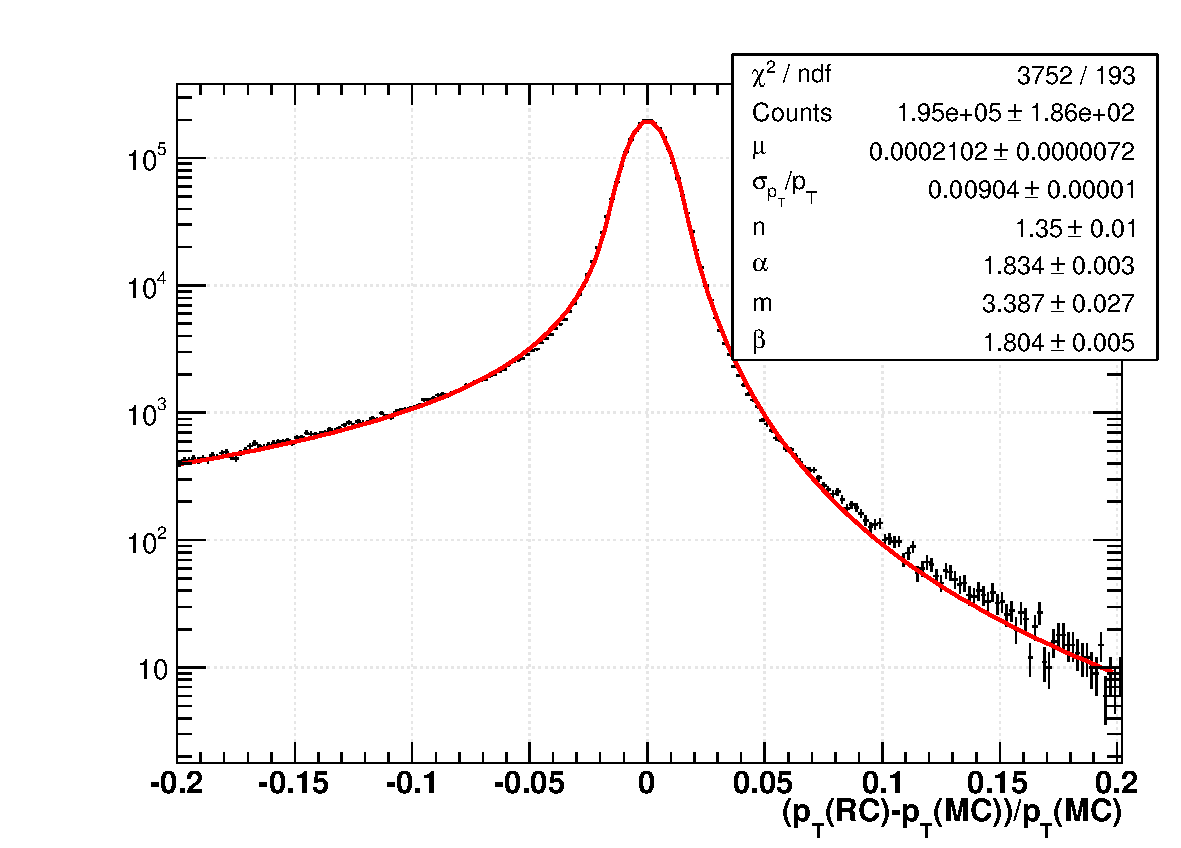
\includegraphics[width=0.45\textwidth]{fig/3.Analysis/Efficiency/momRes/momShape}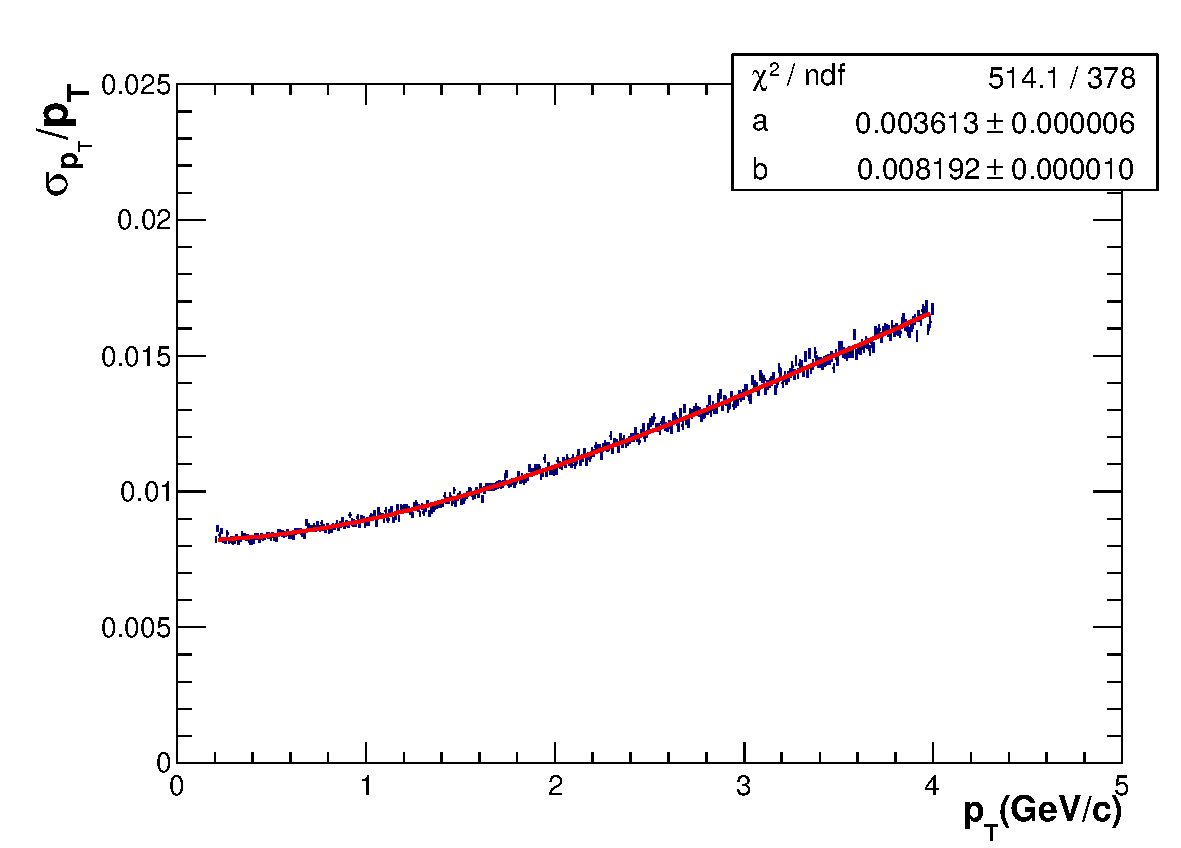
\includegraphics[width=0.45\textwidth]{fig/3.Analysis/Efficiency/momRes/PtRes}
\par\end{centering}

\protect\caption{Left panel shows distribution of $p_{T}^{rec}$ probability at a given
input $p_{T}^{MC}$ from the embedding sample with 1\% momentum resolution.
Right panel show the momentum resolution from the embedding sample.}


\label{fig:mom Res}
\end{figure}



\subsection{Pair efficiency and acceptance }

The pair efficiency was evaluated by Monte Carlo folding method from
the single track efficiency. We used two method folding the pair efficiency
in Au+Au analysis: 
\begin{enumerate}
\item virtual photon decay method, which virtual photons with $M_{ee}$
and $p_{T}$ distributions from the cocktail simulation and a flat
$\eta$, $\phi$ distribution. Then the virtual photon is isotropically
decay into electron pairs.
\item cocktail method, where we used cocktail as input. The input particles
decay into electron pairs following their decay kinematics. The heavy
flavor quark decay process, suck like open charm decay and Drell-Yan
process were from PYTHIA model. This method will be discussed in detail
in next section.
\end{enumerate}
In relativistic heavy-ion collision, we have difficulties in separating
the electrons from heavy flavor quark decay and those produced from
medium. Furthermore, the contribution from heavy flavor decays remains
unclear due to the possible medium modification effect in heavy-ion
collision. This two method served as two extreme approaches of decay
kinematics in the Au+Au collision : virtual photon method is close
to the decay kinematics of medium; cocktail method handles the heavy
flavor decays through PYTHIA model which is similar to the process
in p+p collision. 

The single electron efficiency was folded in for each daughter track
in full 3D ($p_{T}$, $\eta$, $\phi$) momentum space. Their momentum
were smeared by the momentum resolution and energy loss effect (see
section 3.5.2). The pair efficiency was calculated and applied in
2 dimension ($M_{ee}$ vs $p_{T}$ ), within STAR acceptance ($|y_{ee}|<1$,
$p_{T}^{e}>0.2GeV/c$, $|\eta_{e}|<1$). The difference between the
two method is small and we included it into systematic uncertainty.
The photon conversion rejection cut efficiency was calculated by $\pi_{0}$
Dalitz decay embedding sample and included into the pair efficiency,
shown in Figure \ref{fig:phiV eff}. Figure \ref{fig:pair eff} is
a summary of the pair efficiencies as a function of $M_{ee}$ used
in this analysis.

\begin{figure}
\begin{centering}
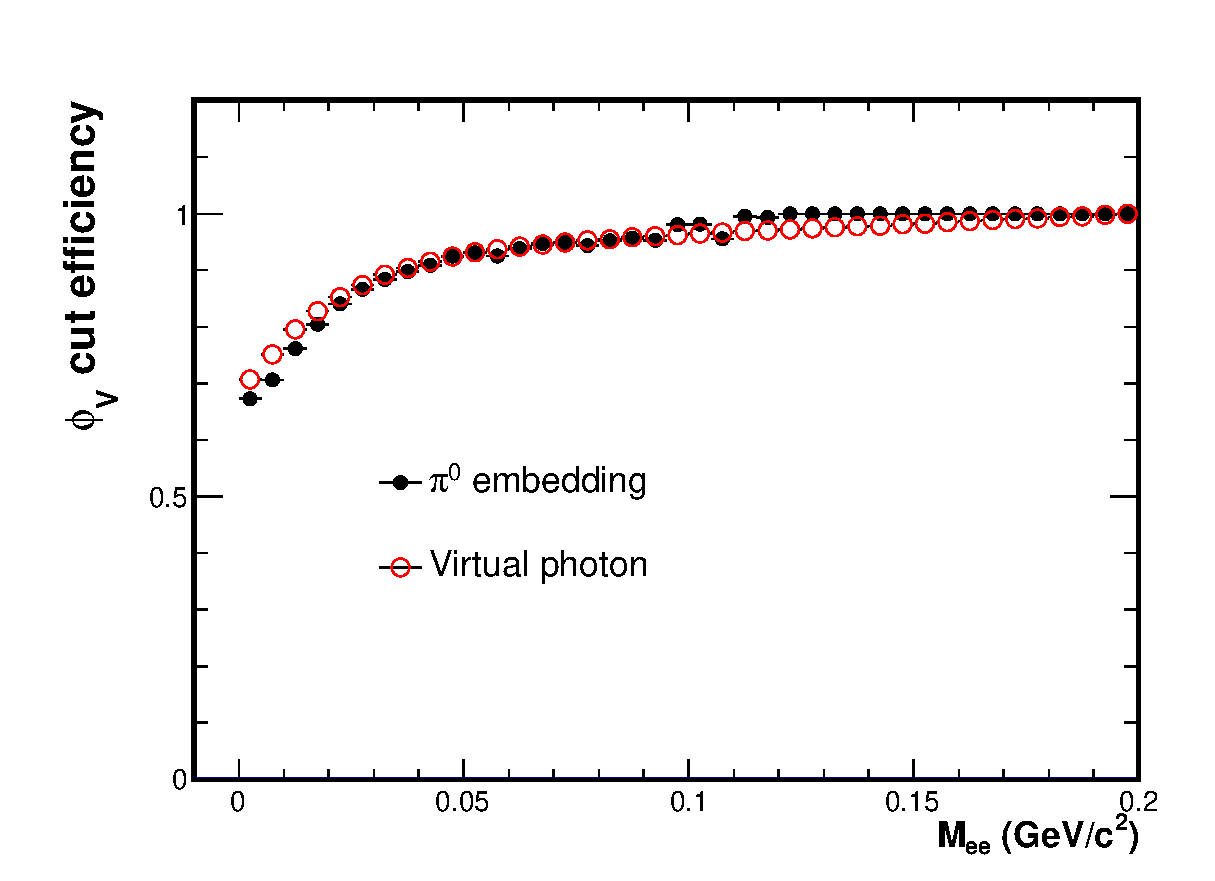
\includegraphics[width=0.5\textwidth]{fig/3.Analysis/Efficiency/phiVeff}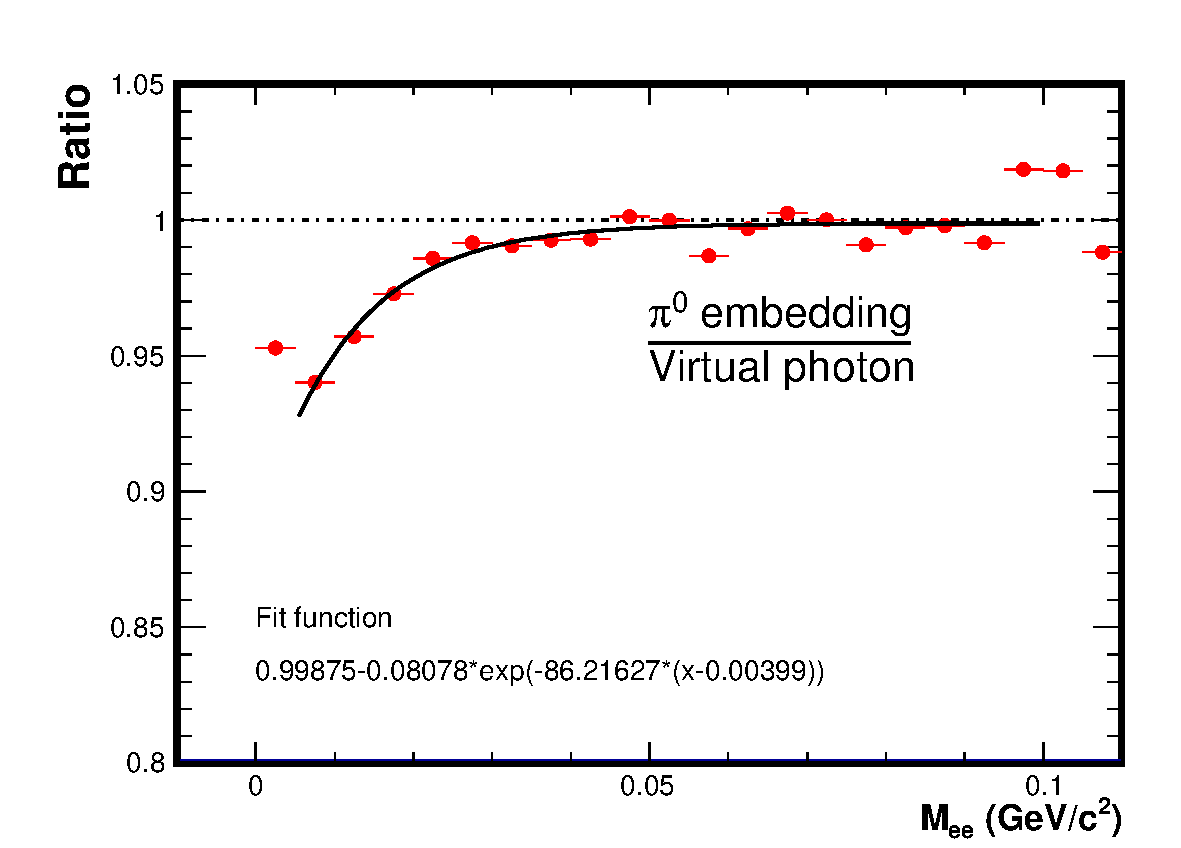
\includegraphics[width=0.5\textwidth]{fig/3.Analysis/Efficiency/comparePi0vsVirtualphoton}
\par\end{centering}

\protect\caption{$\phi_{V}$ efficiency calculated by $\pi^{0}$ Dalitz decay embedding
and virtual photon method (left) and also their comparison (right). }


\label{fig:phiV eff}
\end{figure}


\begin{figure}
\begin{centering}
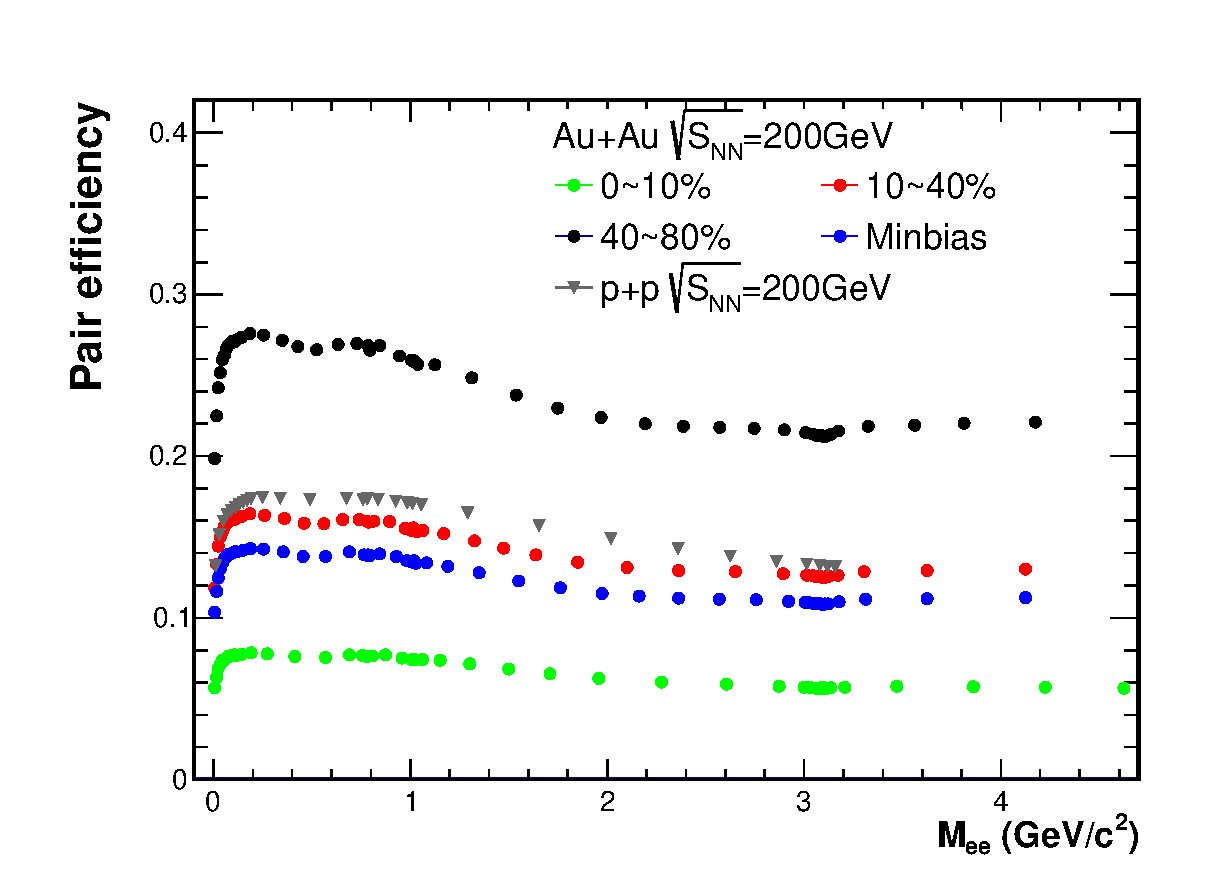
\includegraphics[width=0.5\textwidth]{fig/3.Analysis/Run11/eff_cen}\includegraphics[width=0.5\textwidth]{fig/3.Analysis/Run11/eff_pT}
\par\end{centering}

\protect\caption{(Left) Pair efficiency for different centralities Au+Au collision
and p+p collision. (Right) $p_{T}^{ee}$ dependence of pair efficiency
in Au+Au minimum bias collision.}


\label{fig:pair eff}
\end{figure}
 

In this analysis, the di-electron transverse mass ($m_{T}$) spectra
and their inverse slope parameters were also studied in Au+Au collision,
which need to be corrected for the detector acceptance. The acceptance
correction was calculated as following:

\begin{equation}
\varepsilon_{pair}^{acc}=\frac{dN/dM_{ee}/dy(p_{T}(e)>0.2GeV/c,\,|\eta_{e}|<1,\,|y_{ee}|<1)}{dN/dM_{ee}/dy(|y_{ee}|<1)}\label{eq:eff acc}
\end{equation}
In Figure \ref{fig:eff acc}, the acceptance correction was calculated
by the two methods mentioned previously for Au+Au 200 GeV minimum
bias collisions. There is huge difference between the two method,
especially in intermedia mass region (IMR). It is because di-electrons
are mainly come from charm contribution in this mass region. The two
methods treat the correlation between the daughter pairs quite differently.
In virtual photon method, the correlation between the decay daughters
is come from decay kinematics itself. While in cocktail method, since
the charm component is simulated by PYTHIA, the daughter pairs carry
the strong correlation inherited from charm pairs. Therefore, it leads
to large difference in the acceptance for di-electron pairs. We took
the difference between the two methods as systematic uncertainty in
inverse slope parameters of transverse mass spectra due to leak of
knowledge of this two processes in heavy-ion collisions.

\begin{figure}
\begin{centering}
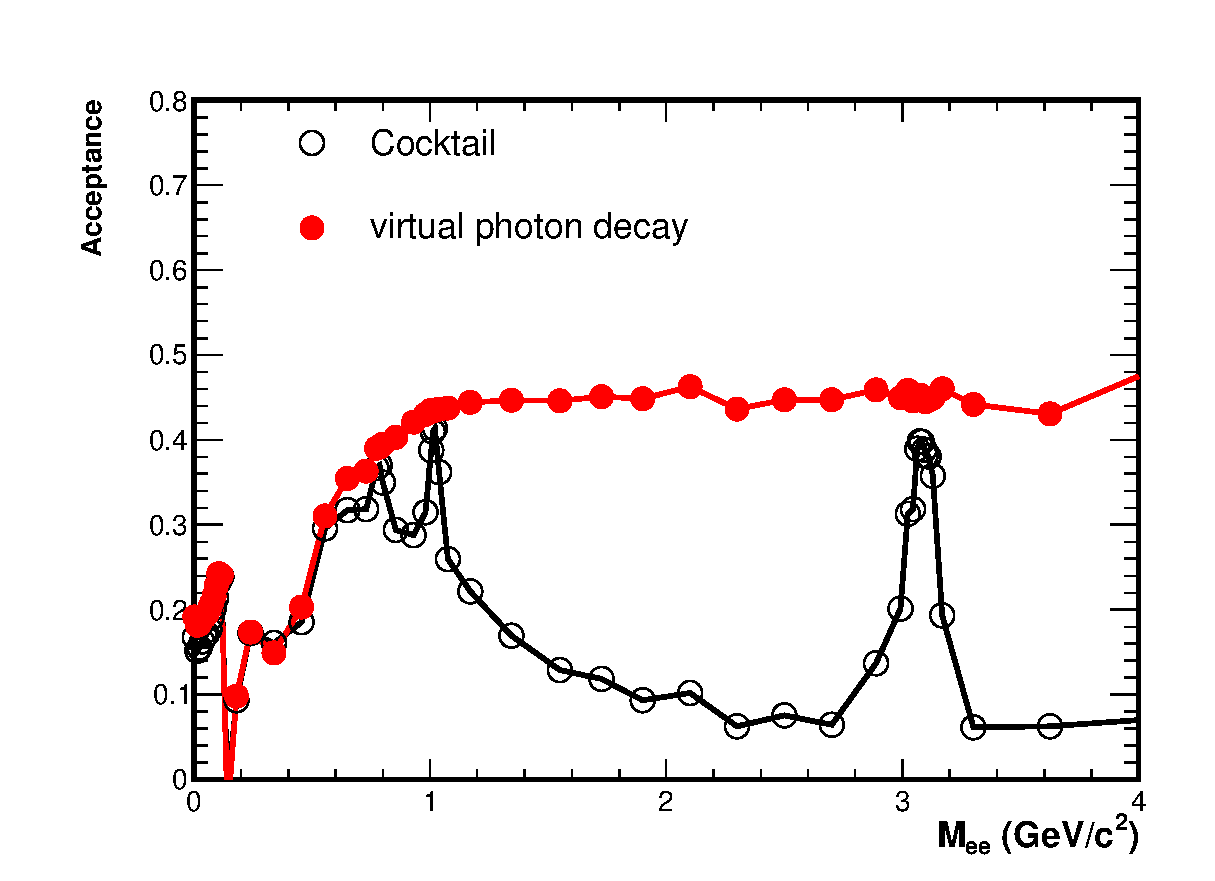
\includegraphics[width=0.8\textwidth]{fig/3.Analysis/Efficiency/Acceptance_mass}
\par\end{centering}

\protect\caption{Acceptance correction calculated by virtual photon method and cocktail
method for Au+Au 200GeV collision.}


\label{fig:eff acc}
\end{figure}



\subsection{Trigger efficiency and trigger bias}

The event sample selection is required by a VPD coincidence and a
valid primary vertex. Due to the inefficiency of the VPD detector
in p+p collisions, we need correct the possible bias of trigger and
vertex selection. In this analysis, trigger bias correction factor
was taken from \cite{PhysRevC.86.024906}, the number is 64\% with
8\% systematic uncertainty.


\subsection{The total correction factors for di-electron spectra}

Finally, the di-electron continuum raw yield within STAR acceptance
are corrected as following:

\begin{equation}
Y(M_{ee},p_{T})=\frac{N_{raw}(M_{ee},p_{T})}{dM_{ee}dy\times\varepsilon_{pair}(M_{ee},p_{T})}\times f_{triggerbias}\label{eq:yield correction}
\end{equation}
, where $N_{raw}$ is the di-electron raw yields within STAR acceptance,
$\varepsilon_{pair}$ is the efficiency correction and $f_{triggerbias}$
is the trigger bias factor (\textasciitilde{}64\% in p+p collisions,
\textasciitilde{}1 in Au+Au collisions).


\section{Hadronic cocktails}

The di-electron signals observed in experiment are produced from various
sources during the system evolution. After chemical freeze out, di-electron
pairs from long life meson and hadron decays contribute mainly to
the di-electron signal. These components, which is usually called
``Hadronic cocktails'', can be well understood by measuring the
corresponding decay channels. In this analysis, cocktails contain
contributions from decays and Dalitz decays of $\pi^{0}$, $\eta$,
$\eta'$, $\rho$ (only in p+p collisions), $\omega$, $\phi$, $J/\psi$,
$\psi'$, $c\bar{c}$, $b\bar{b}$ and Drell-Yan (DY) production. 

The cocktail for p+p collision is taken from STAR published result
\cite{PhysRevC.86.024906}, and the charm cross section is updated
to $797\pm210(stat.)_{-295}^{+208}(sys.)\mu b$ with respect to the
newest published result from STAR \cite{PhysRevD.86.072013}. Figure
\ref{fig: cocktail Input} left panel shows the input hadron $p_{T}$
spectra for p+p collision. Figure \ref{fig:cocktailpp} shows the
cocktail for p+p collisions.

We used the similar cocktail simulation methods for Au+Au 200 GeV
collision as we used in p+p collision \cite{PhysRevC.86.024906}.
The cocktail simulation only contains the hadron form-factor decays
in the vacuum at freeze-out. For the $\rho$ component, we included
a vacuum $\rho$ calculation only when comparing data with cocktails
including the vacuum $\rho$. We assumed a flat rapidity distribution
within $|y|<1$ for the input hadrons. Table \ref{table:CK AuAuinput}
lists the $dN/dy$ (or cross-section), branching ratios, uncertainty
and reference for all input sources. The hadron spectra measured by
STAR and PHENIX were parameterized by the simultaneous Tsallis Blast-Wave
(TBW) model fit \cite{PhysRevC.79.051901}. Figure \ref{fig: cocktail Input}
right panel shows the TBW fit results for all input hadron spectra
except $J/\psi$. The cocktail input for $J/\psi$ was taken from
the measurement by the PHENIX collaboration \cite{PhysRevC.81.034911}.
For light hadrons, the TBW fit provides good parameterizations to
these measure spectra. The same core TBW parameters was used to predicted
the spectral shapes for these components without measurements (e.g.
low $p_{T}$ $\eta$, $\eta'$, $\omega$).

The correlated charm, bottom and Drell-Yan contributions were studied
by PYTHIA simulation \cite{Torbjorn-Sjostrand:2001ek} and scaled
by the number of binary collisions ($N_{bin}$) in Au+Au collisions.
We used PYTHIA 6.419 with settings: MSEL=1, PARP(91) ($\left\langle k_{\perp}\right\rangle $)
= 1.0 GeV/$c$ and PARP(67) (parton shower level) = 1.0, which was
tuned to match STAR measured charmed meson spectrum in p+p collisions
\cite{PhysRevD.86.072013}. The input charm cross section was also
taken from the charmed meson measurement.

The detector resolution was also taken into account by smearing the
daughter electron's momentum with the method discussed in section
3.5. Finally, the di-electron pair mass distributions from the sources
are normalized by branching ratios and the measured $dN/dy$. Figure
\ref{fig:cocktailAuAu} shows the cocktails for Au+Au 200 GeV minimum
collisions.

The cocktails were also simulated in difference centrality bins (0\textasciitilde{}10\%,
10\textasciitilde{}40\% and 40\textasciitilde{}80\%). The similar
TBW model fit was applied to parameterize the measured spectra in
corresponding centrality bins. For hadron without measurement, the
TBW predictions were used as the input $p_{T}$ distributions. We
used the relative pion yields ($R_{\pi}$) with respect to minimum
bias collisions (0\textasciitilde{}80\% centrality bin) as scale factor
for the input $dN/dy$ in each centrality bin. The correlated charm
contributions were scaled by the relative number of binary collisions
($R_{N_{bin}}$). Table \ref{table: scale cocktail} summarizes all
these scale factors.

\begin{table}
\begin{centering}
\begin{tabular}{c|c|c|c|c}
\hline 
source & B.R. & $dN/dy$ or $\sigma$ & Uncertainty & Reference\tabularnewline
\hline 
\hline 
$\pi^{0}\rightarrow\gamma ee$ & $1.174\times10^{-2}$ & 98.5 & 8\% & STAR \cite{PhysRevLett.92.112301,PhysRevLett.97.152301}\tabularnewline
$\eta\rightarrow\gamma ee$ & $7\times10^{-3}$ & 7.86 & 30\% & PHENIX \cite{PhysRevC.81.034911}\tabularnewline
$\eta'\rightarrow\gamma ee$ & $9\text{×}10^{\text{−}4}$ & 2.31 & 100\% & PHENIX \cite{PhysRevC.81.034911}\tabularnewline
$\rho\rightarrow ee$ & $4.72\times10^{-5}$ & 9.88 & 42\% & STAR \cite{PhysRevLett.92.092301}\tabularnewline
$\omega\rightarrow ee$ & $7.28\text{×}10^{\text{−}5}$ &  &  & \tabularnewline
$\omega\rightarrow\pi^{0}ee$ & $7.7\text{×}10^{\text{−}4}$ & 9.87 & 33\% & STAR \cite{STAR-Collaboration:2012wq}\tabularnewline
$\phi\rightarrow ee$ & $2.95\text{×}10^{\text{−}4}$ &  &  & \tabularnewline
$\phi\rightarrow\eta ee$ & $1.15\text{×}10^{\text{−}4}$ & 2.43 & 10\% & STAR \cite{Adams2005181}\tabularnewline
$J/\psi\rightarrow ee$ & $5.94\text{×}10^{\text{−}2}$ & $2.33\times10^{-3}$ & 15\% & PHENIX \cite{PhysRevLett.98.232301}\tabularnewline
$\psi'\rightarrow ee$ & $7.72\text{×}10^{\text{−}3}$ & $3.38\text{×}10^{\text{−}4}$ & 27\% & PHENIX \cite{al.:kb,daSilva2009227c}\tabularnewline
\hline 
\hline 
$c\bar{c}\rightarrow ee$ & $1.03\text{×}10^{\text{−}1}$ & $d\sigma^{c\bar{c}}/dy=170\mu b$ & 35\% & STAR \cite{PhysRevD.86.072013}\tabularnewline
$b\bar{b}\rightarrow ee$ & $1.08\text{×}10^{\text{−}1}$ & $\sigma_{pp}^{b\bar{b}}=3.7\mu b$ & 30\% & Pythia \cite{Torbjorn-Sjostrand:2001ek}\tabularnewline
Drell-Yan & $3.36\text{×}10^{\text{−}2}$ & $\sigma_{pp}^{DY}=42nb$ & 30\% & Pythia \cite{Torbjorn-Sjostrand:2001ek}\tabularnewline
\hline 
\end{tabular}
\par\end{centering}

\protect\caption{Inputs of various cocktail components for Au+Au 200 GeV minimum bias
collisions. }


\label{table:CK AuAuinput}
\end{table}


\begin{table}
\begin{centering}
\begin{tabular}{c|c|c|c|c}
\hline 
centrality & $\pi$ \emph{$dN/dy$} & $R_{\pi}$ & $\left\langle N_{bin}\right\rangle $ & $R_{N_{bin}}$\tabularnewline
\hline 
\hline 
0\textasciitilde{}80\% & 98.49 & 1 & $291.90\pm20.46$ & 1\tabularnewline
\hline 
0\textasciitilde{}10\% & 279.2 & 2.834 & $941.24\pm26.27$ & 3.224\tabularnewline
\hline 
10\textasciitilde{}40\% & 131.1 & 1.331 & $391.36\pm30.21$ & 1.341\tabularnewline
\hline 
40\textasciitilde{}80\% & 30.45 & 0.309 & $56.62\pm13.62$ & 0.194\tabularnewline
\hline 
\end{tabular}
\par\end{centering}

\protect\caption{Scale factors for centrality dependent cocktails.}


\label{table: scale cocktail}
\end{table}


\begin{figure}
\begin{centering}
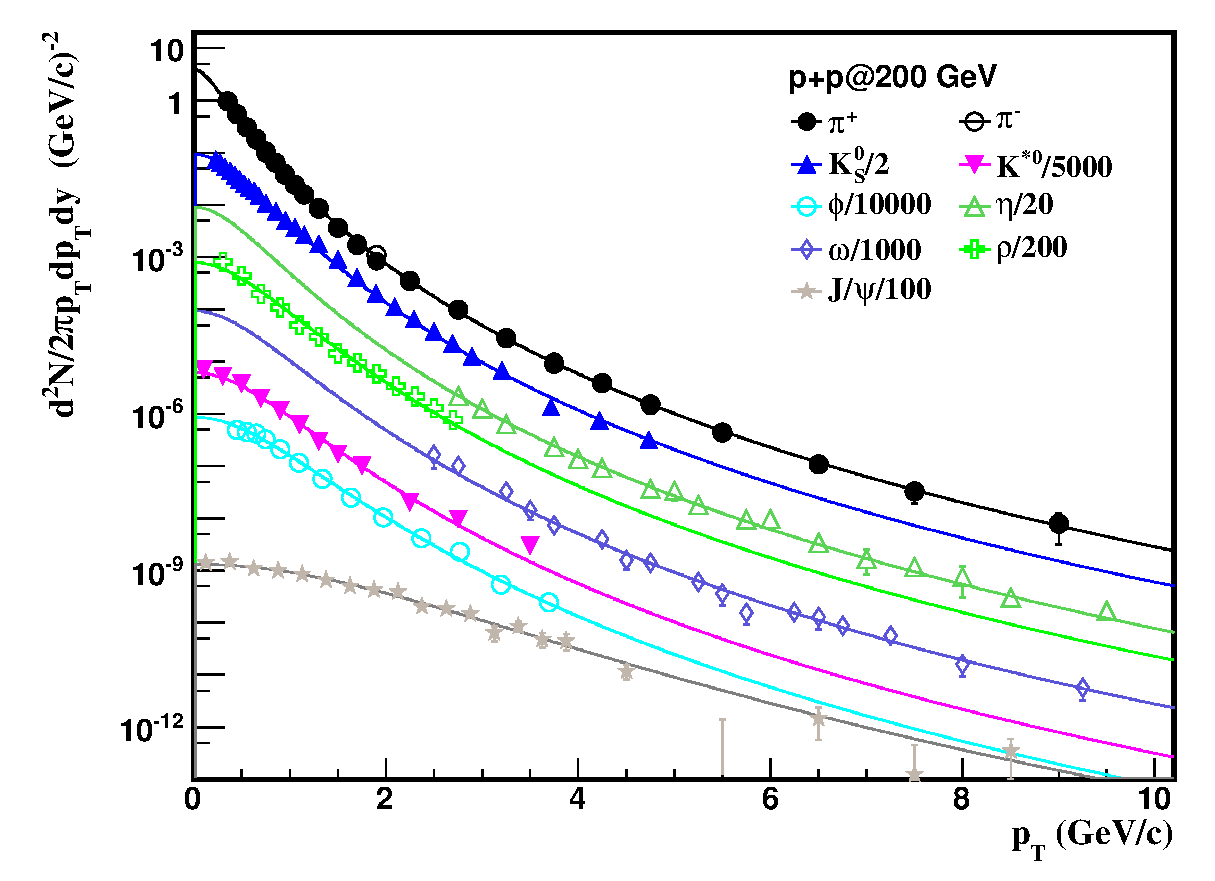
\includegraphics[width=0.45\textwidth]{fig/3.Analysis/cocktail/11PLUS1mesons_pp_woProton_allPt_new}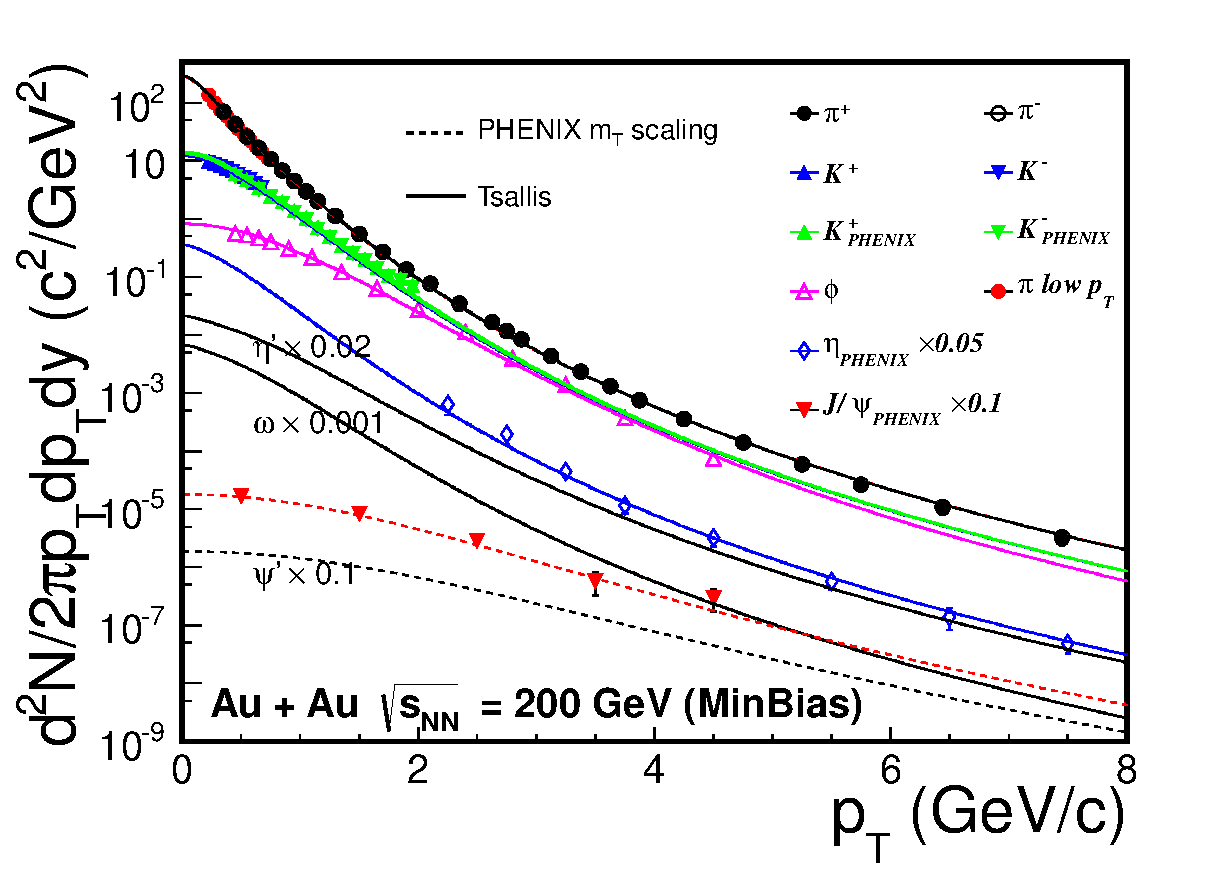
\includegraphics[width=0.45\textwidth]{fig/3.Analysis/cocktail/AuAu200_inputpT}
\par\end{centering}

\protect\caption{Left panel: the invariant yields of measured mesons fit with the Tsallis
functions in p+p 200 GeV collision \cite{PhysRevC.86.024906}. The
solid lines represent the fit. Right panel: invariant yields of mesons
in Au+Au collision at $\sqrt{s_{NN}}=200$ GeV. The solid lines represent
the simultaneous Tsallis Blast-Wave (TBW) fit to the measure data
points and TBW predictions for $\eta$, $\eta'$, $\omega$ with the
same set of fit parameters. The dash lines depict the same parametrization
to the measures $J/\psi$ spectrum and the predicted $\psi'$ spectrum
as in \cite{PhysRevC.81.034911}.}


\label{fig: cocktail Input}
\end{figure}


\begin{figure}
\begin{centering}
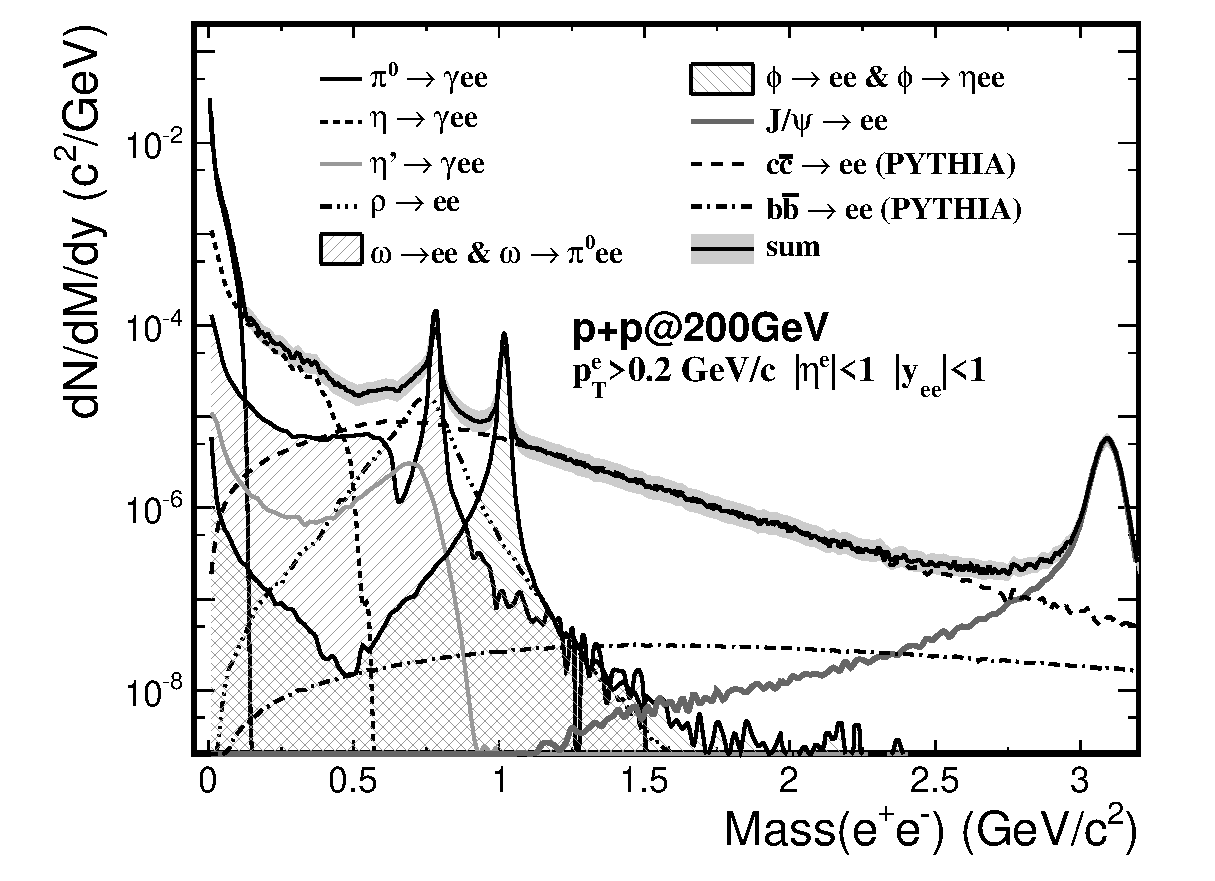
\includegraphics[width=0.8\textwidth]{fig/3.Analysis/cocktail/bcCocktail}
\par\end{centering}

\protect\caption{Cocktails for p+p 200 GeV minimum bias collision.}


\label{fig:cocktailpp}

\end{figure}


\begin{figure}
\begin{centering}
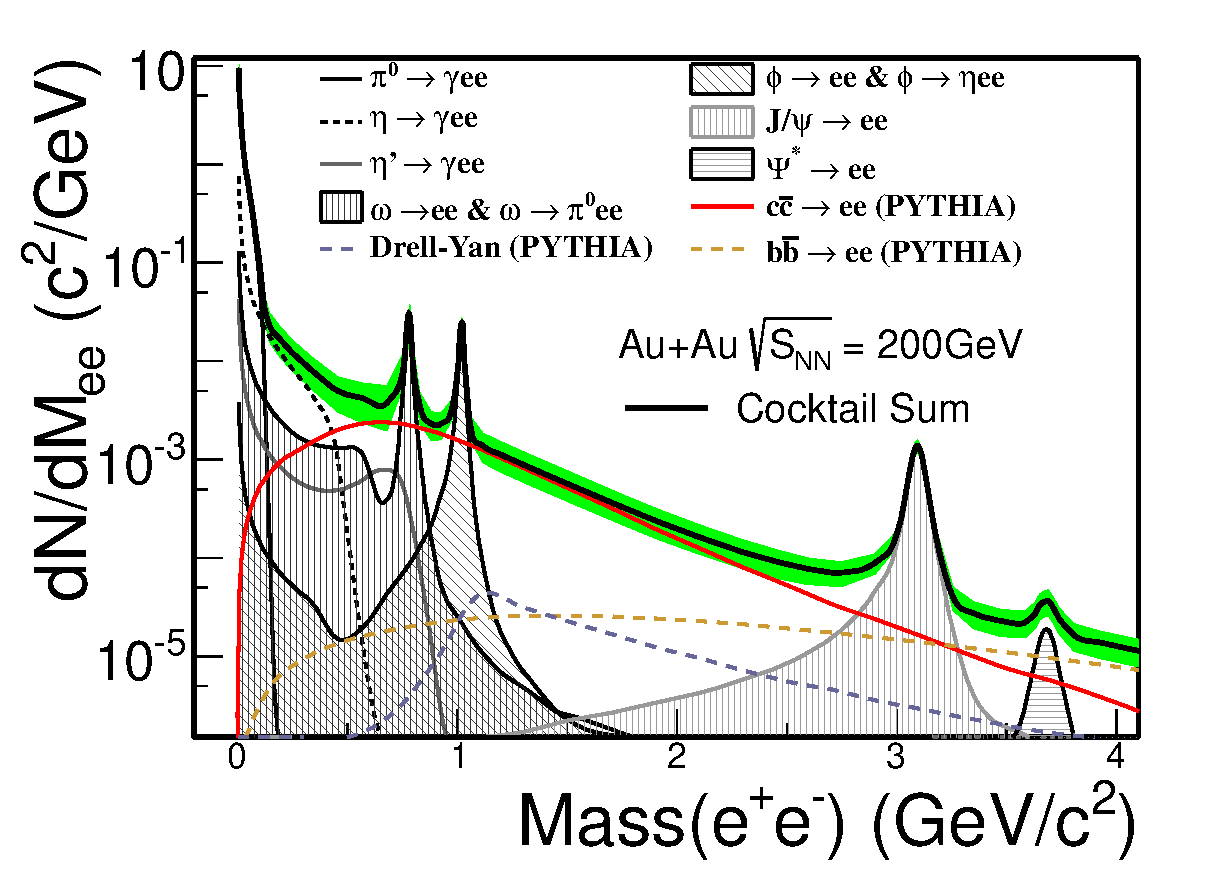
\includegraphics[width=0.8\textwidth]{fig/3.Analysis/cocktail/cocktailmb_PRL}
\par\end{centering}

\protect\caption{Cocktails for Au+Au 200GeV minibias collision. The green band depicts
the systematics uncertainty.}


\label{fig:cocktailAuAu}
\end{figure}



\section{Systematic uncertainty}

In this analysis, the systematic uncertainty was split into two main
parts: from data analysis which is highly correlated with $M_{ee}$
, and from efficiency which is uncorrelated with $M_{ee}$.

The systematic uncertainties source from data analysis are listed
below:
\begin{enumerate}
\item Background, including uncertainties of the acceptance factor for like-sign
background ($M_{ee}<M_{th}$)and the normalization for mixed event
background ($M_{ee}>M_{th}$).
\item Like-sign residue, the uncertainty from the fit to parameterize the
difference between like-sign and mixed event background in mass region
$M_{ee}>M_{th}$.
\item Hadron contamination.
\end{enumerate}
The uncertainty from acceptance factor was come from difference between
1D ($p_{T}$) and 2D ($M_{ee}$vs $p_{T}$) acceptance factor correction
as mentioned in section 3.4.1. The normalization uncertainty was studied
by changing the normalization regions around which used in the analysis,
and the difference was taken as systematic uncertainty. For p+p collision
the normalization regions was changed to 0.3\textasciitilde{}0.8 $GeV/c^{2}$
and 0.5\textasciitilde{}1.2 $GeV/c^{2}$, while in Au+Au collision
it was changed to 0.75\textasciitilde{}1.75 $GeV/c^{2}$ and 1.25\textasciitilde{}3
$GeV/c^{2}$. As mentioned in section 3.4.2, we used function \ref{eq:LSresidue}
to parameterized the correlated residue and subtract it additionally
from the foreground. The 68\% confidence level of the fit was taken
as systematic uncertainty (Figure \ref{fig:LS/Mix}). 

Hadron contamination was studied by mixing pure hadron sample into
electron sample, we called it the mixed sample. The hadron sample
was weighted by the ratio of hadron yield over electron yield from
the electron purity study (Figure \ref{fig:h/e ratio}). The particles
in the mixed sample were randomly paired with each other. There are
three condition: e-e pairs, this is di-electron signal; e-h and h-h
contamination pairs. Then the same background subtraction was done
to the mixed sample. Finally, we used function \ref{eq:h contamination}
to parameterize yields of the contamination pairs and calculated its
contribution to systematic uncertainty (Figure \ref{fig: h contamination}
).

Finally, we combined all these source and plotted the systematic uncertainty
from data analysis in Fig \ref{fig:sys AuAu} and \ref{fig:sys pp}.

\begin{equation}
f(x)=\begin{cases}
a_{0}+a_{1}x+a_{2}x^{2}+a_{3}x^{3} & x<x_{th}\\
b\exp(cx) & x>x_{th}
\end{cases}\label{eq:h contamination}
\end{equation}
The efficiency uncertainties have already been discussed in section
3.5. Table \ref{table: sys eff}.

\begin{table}
\begin{centering}
\begin{tabular}{c|c|c|c}
\hline 
 &  & Au+Au & p+p\tabularnewline
\hline 
 & component & Systematic Uncertainty & Systematic Uncertainty\tabularnewline
\hline 
\hline 
TPC & nHitsFits (15-25) & 3.2\% & 0.9\%\tabularnewline
\hline 
 & dca (1.5-0.5cm) & 1.4\% & 1.8\%\tabularnewline
\hline 
 & ndEdxFits & 2\% & 2\%\tabularnewline
\hline 
\hline 
TOF & matching & 5.5\% & 8\%\tabularnewline
\hline 
 & $1/\beta$ & 1.7\% & 0.7\%\tabularnewline
\hline 
total &  & 7.3\% & 8.3\%\tabularnewline
\hline 
pair total &  & 14.6\% & 16.6\%\tabularnewline
\hline 
\end{tabular}
\par\end{centering}

\protect\caption{Systematic uncertainty from efficiency.}


\label{table: sys eff}

\end{table}


\begin{figure}
\begin{centering}
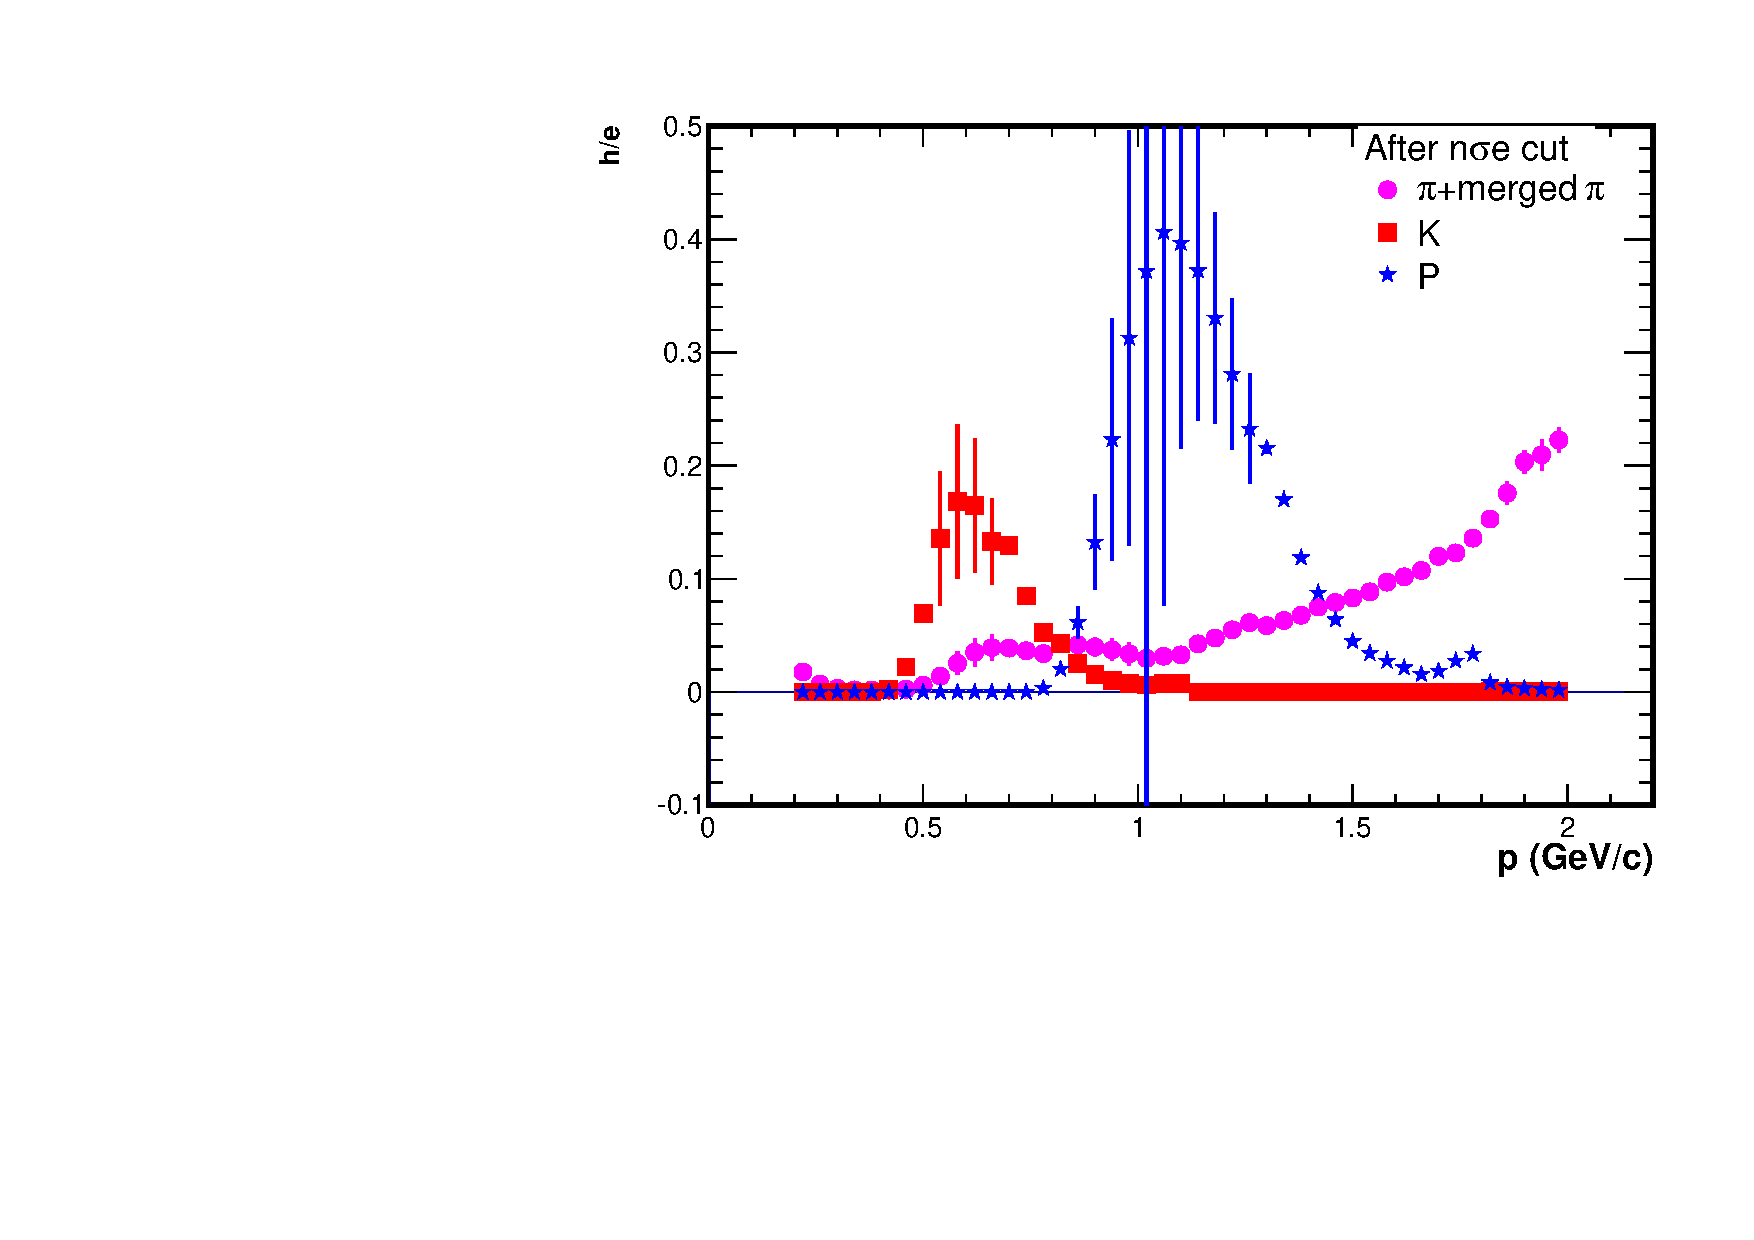
\includegraphics[angle=270,width=0.8\textwidth]{fig/3.Analysis/Additional/purity/hadron2Eratio_3}
\par\end{centering}

\protect\caption{Ratio of hadron yields over electron yields as a function of momentum.}


\label{fig:h/e ratio}

\end{figure}


\begin{figure}
\begin{centering}
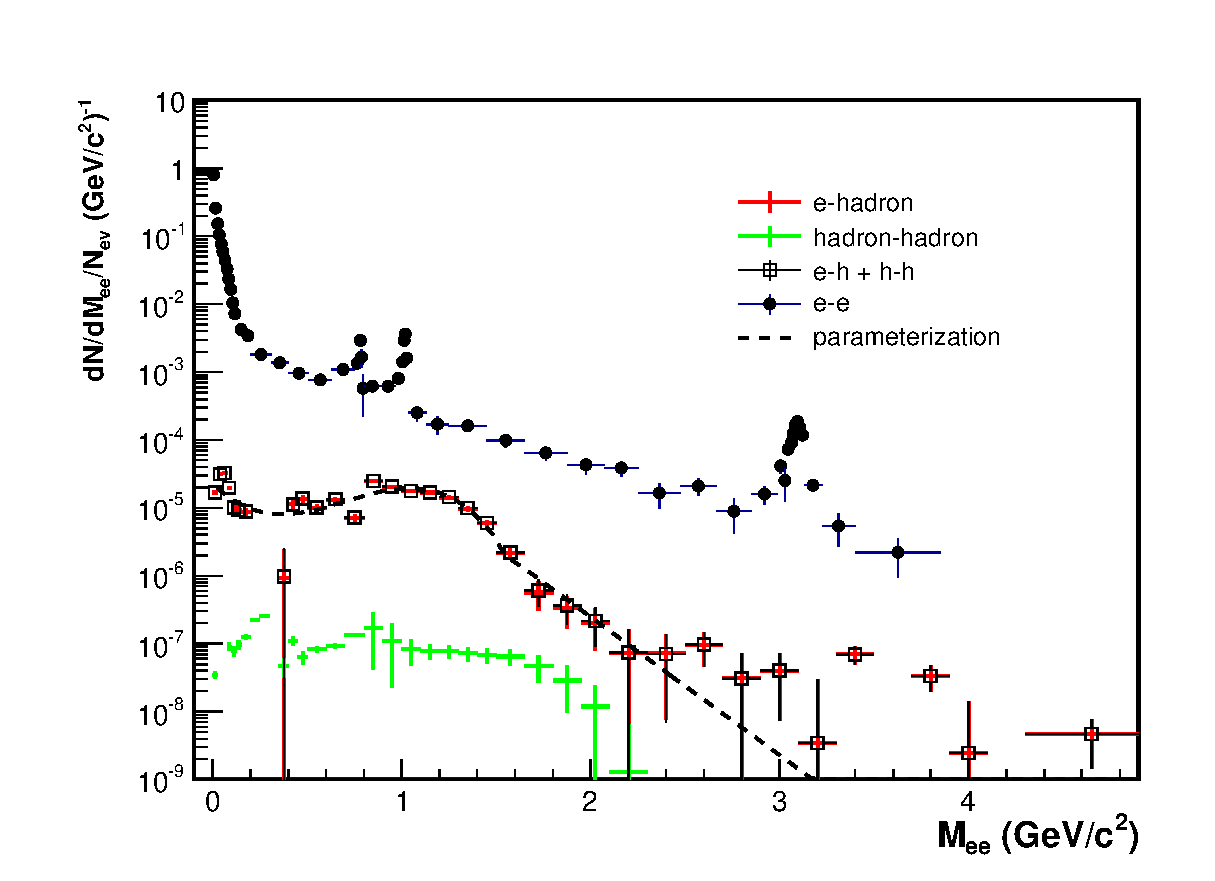
\includegraphics[width=0.8\textwidth]{fig/3.Analysis/SysUncertainty/HardonCondeminationAuAu}
\par\end{centering}

\protect\caption{Yields of di-electron signal pairs, e-h and h-h contamination pairs.}


\label{fig: h contamination}

\end{figure}


\begin{figure}
\begin{centering}
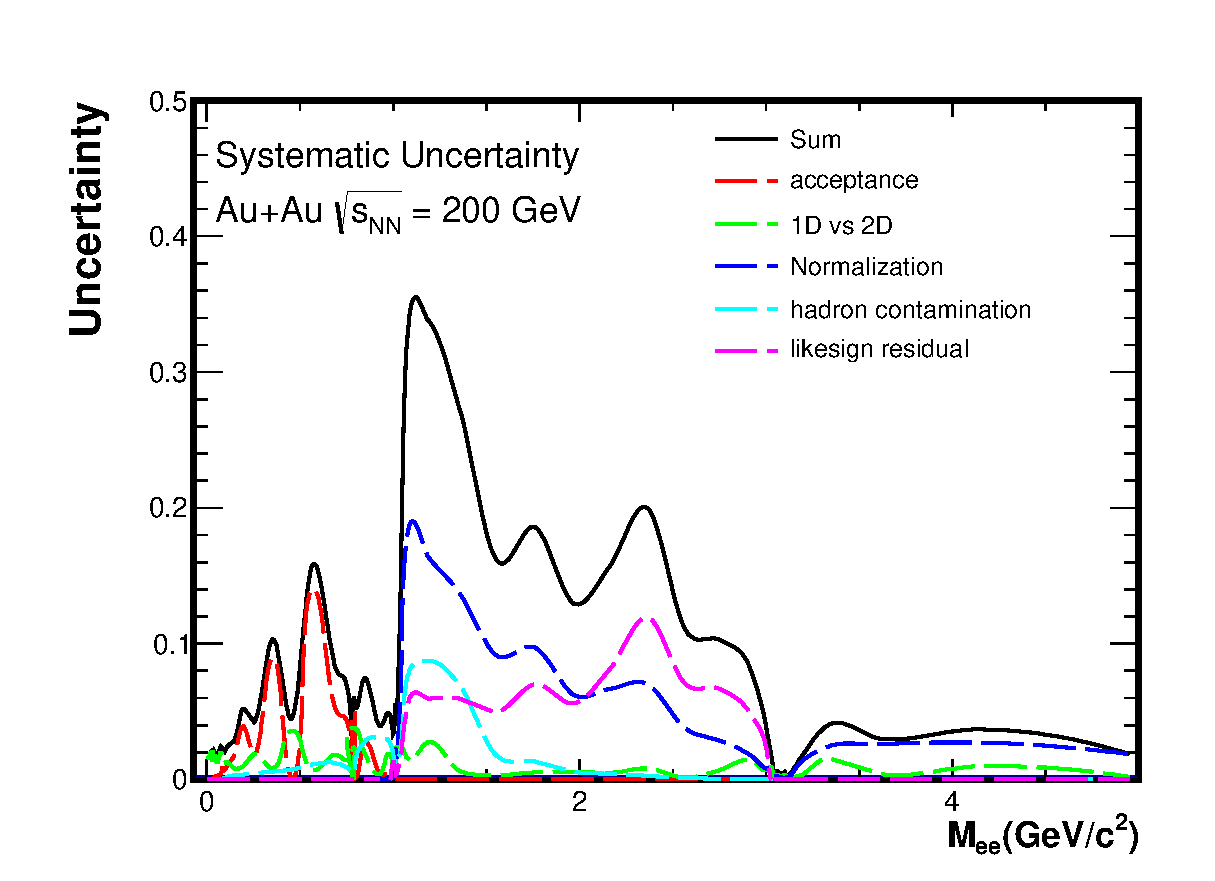
\includegraphics[width=0.8\textwidth]{fig/3.Analysis/SysUncertainty/sysErr_AuAu}
\par\end{centering}

\protect\caption{Systematic uncertainty from data analysis for Au+Au 200GeV minimum
bias collision.}


\label{fig:sys AuAu}

\end{figure}


\begin{figure}
\begin{centering}
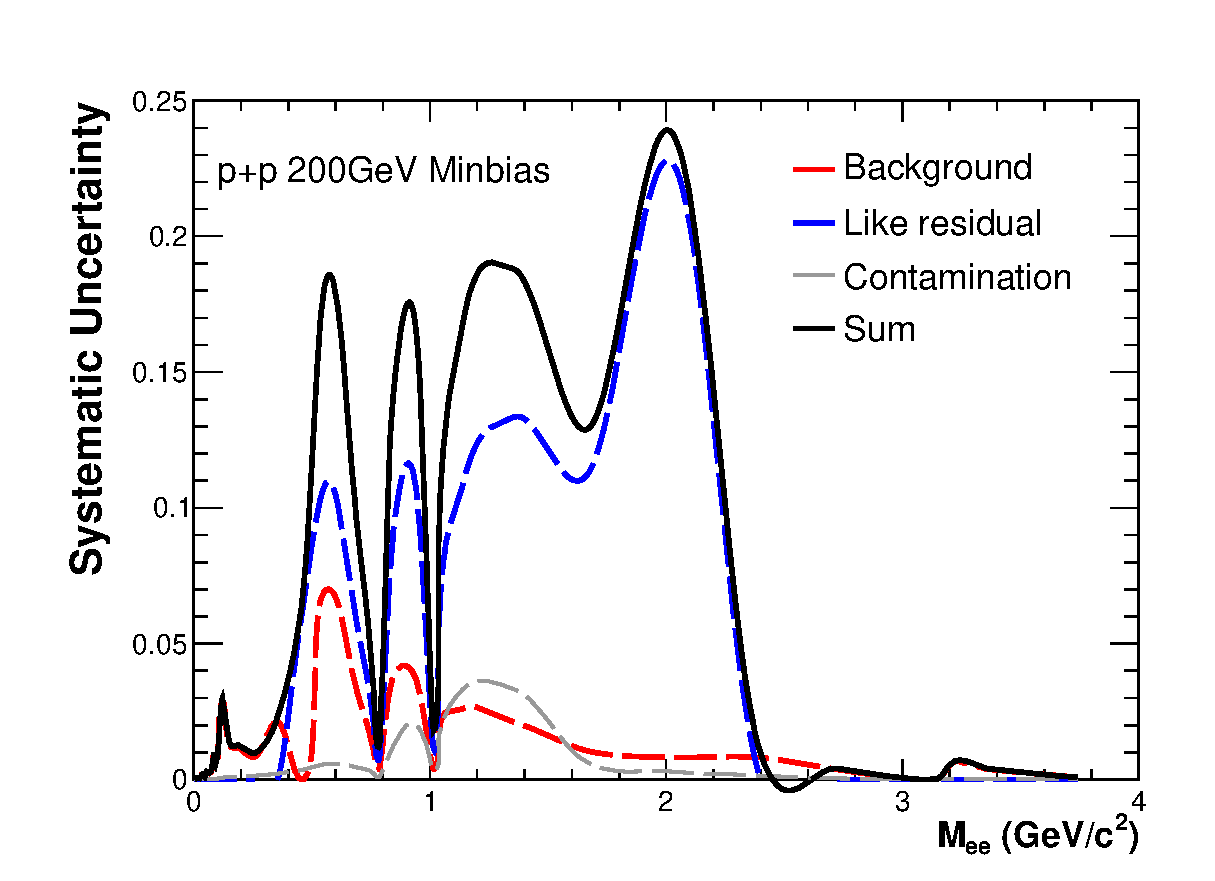
\includegraphics[width=0.8\textwidth]{fig/3.Analysis/SysUncertainty/sysErr_PP}
\par\end{centering}

\protect\caption{Systematic uncertainty from data analysis for p+p 200GeV minimum bias
collision.}


\label{fig:sys pp}

\end{figure}



\section{Combine the Au+Au results from year 2010 and year 2011}

To achieve better statistics, we combined the results from year 2010
and year 2011 together for Au+Au 200 GeV collisions. The year 2010
result has already published in PRL \cite{PhysRevLett.113.022301}.


\subsection{Comparison }

Before combined the data, we compared the results from year 2010 and
year 2011. Figure \ref{fig: Run10vsRun11 cen} and \ref{fig: Run10vsRun11 pT}
show the comparison of the two years results in different centralities
and $p_{T}$ regions. The efficiency correction was done separately
for each year's results by the same process mentioned in section 3.5.
The results are reported within the STAR acceptance ($|y_{ee}|<1$,
$p_{T}^{e}>0.2GeV/c$, $|\eta_{e}|<1$) and show good consistency
with each other within uncertainty. 

\begin{figure}
\begin{centering}
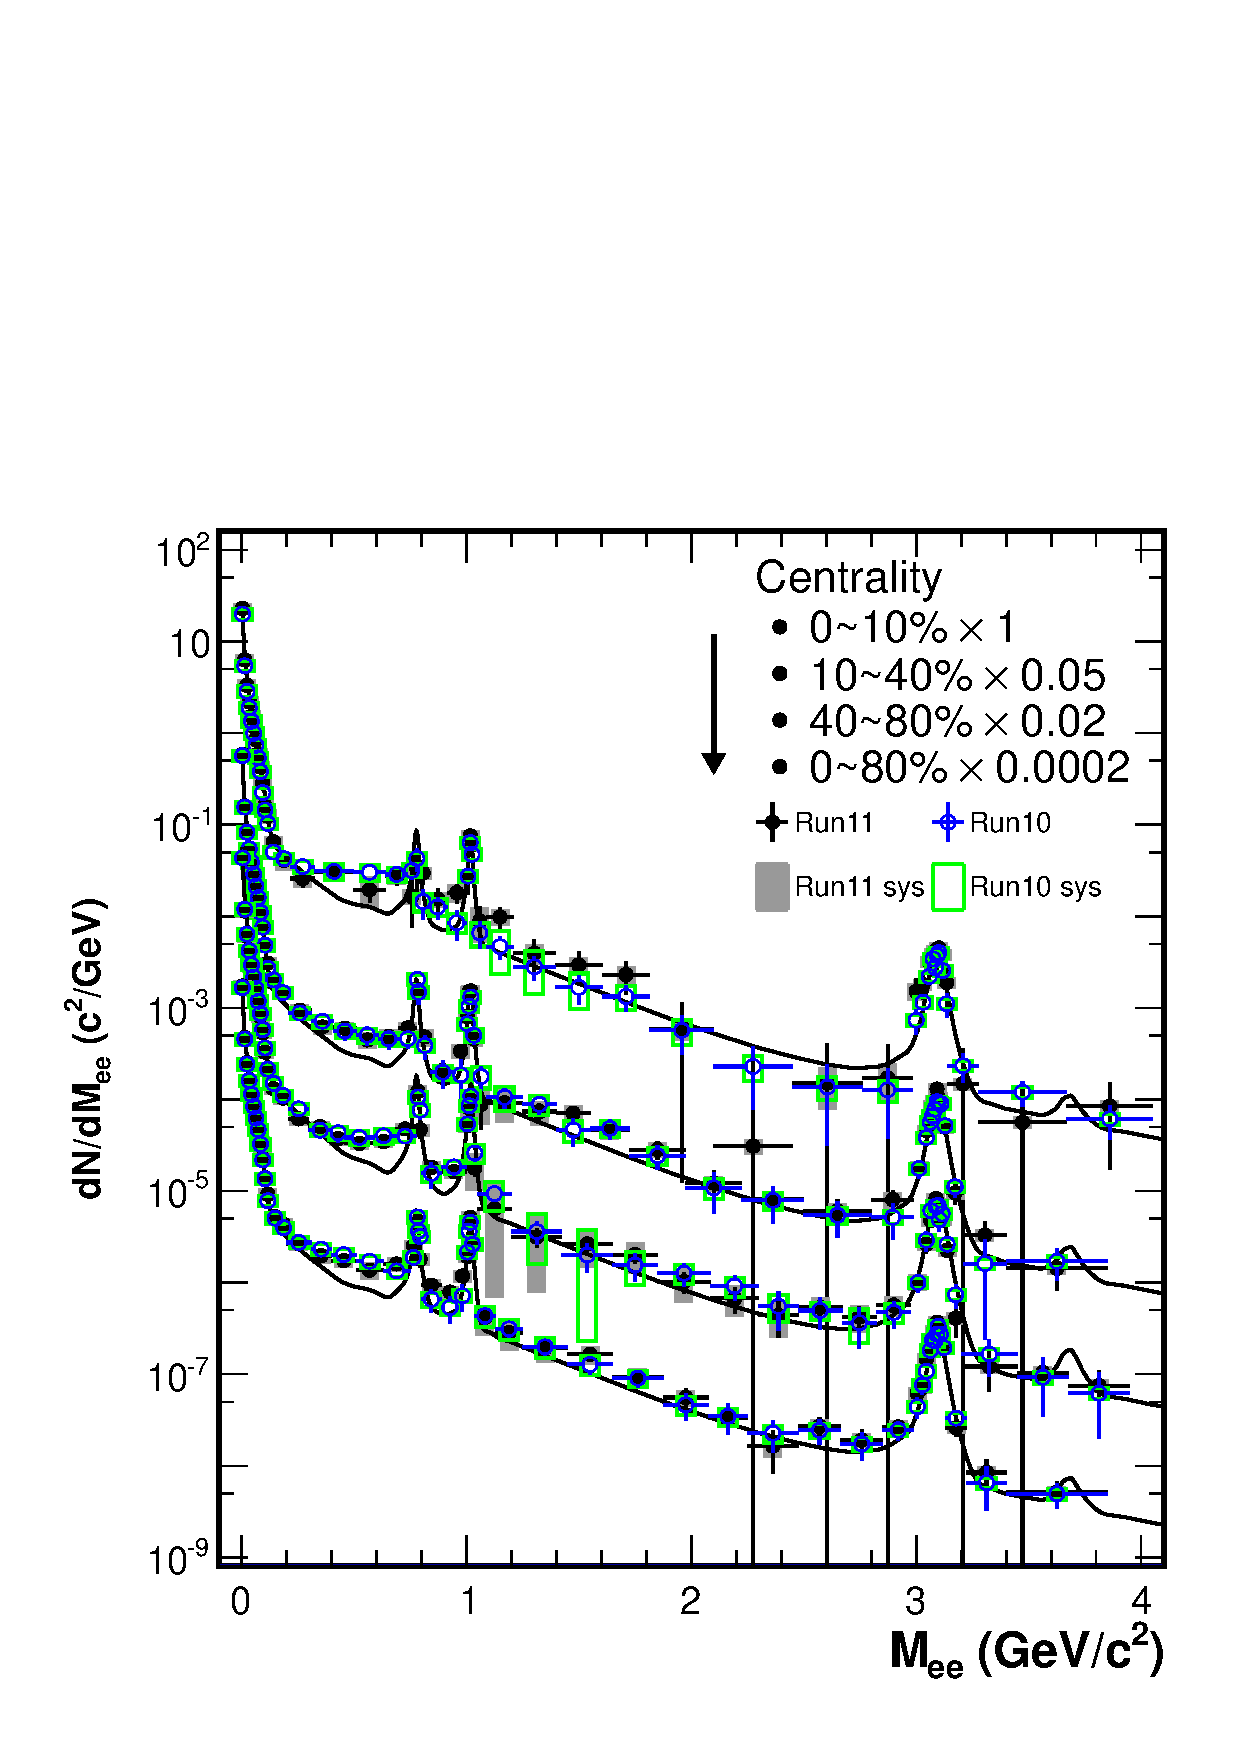
\includegraphics[width=0.45\textwidth]{fig/3.Analysis/Run11/Cen_Yield_cocktail_Run11vsRun10}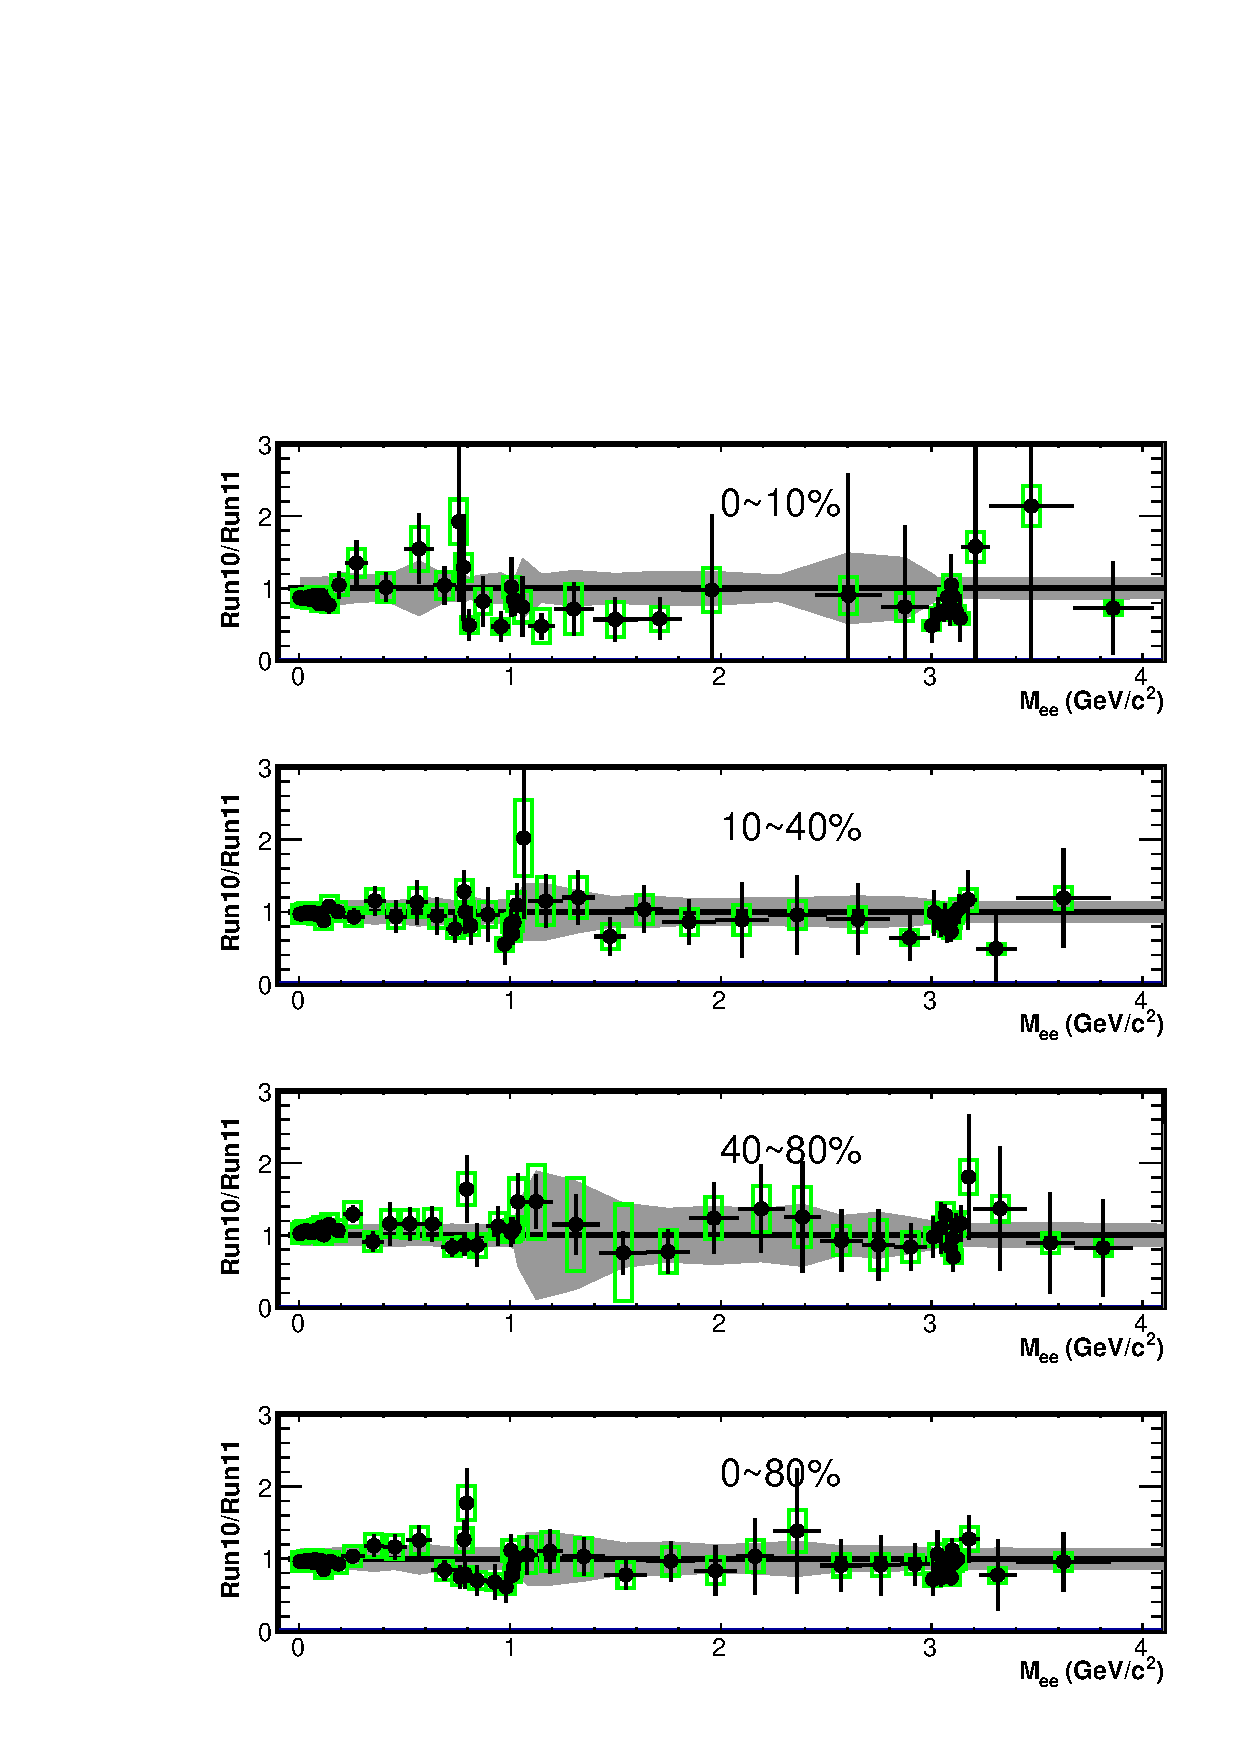
\includegraphics[width=0.45\textwidth]{fig/3.Analysis/Run11/cen_ratio_Run11vsRun10_Run11vsRun10}
\par\end{centering}

\protect\caption{Comparison between Au+Au results from year 2010 and year 2011 in different
centralities. Right panel shows the ratio of year 2010's results over
year 2011's result. The green box depicts the systematic uncertainty
for year 2010's results, and the grey bar represents the systematic
uncertainty for year 2011's results.}


\label{fig: Run10vsRun11 cen}

\end{figure}


\begin{figure}
\begin{centering}
\includegraphics[width=0.45\textwidth]{fig/3.Analysis/Run11/pT_Yield_cocktail_Run11vsRun10}\includegraphics[width=0.45\textwidth]{fig/3.Analysis/Run11/pT_ratio_Run11vsRun10}
\par\end{centering}

\protect\caption{Comparison between Au+Au results from year 2010 and year 2011 in different
$p_{T}$ bins in minimum bias collision. Right panel shows the ratio
of year 2010's results over year 2011's result. The green box depicts
the systematic uncertainty for year 2010's results, and the grey bar
represents the systematic uncertainty for year 2011's results.}


\label{fig: Run10vsRun11 pT}

\end{figure}



\subsection{Combination}

Year 2010's and year 2011's results were combined statistically and
systematically. For the 0\textasciitilde{}10\% centrality bin, since
Run 10 have dominate statistics, we didn't combine Run10 and Run11
data in this centrality to ensure the systematics uncertainty is under
control. 

The data points and their statistical errors were combined by standard
error propagate formula, see Eq. \ref{eq: com stat}, where \emph{Y
\textasciitilde{} yield, w \textasciitilde{} weight and $\delta$
\textasciitilde{} statistic uncertainty.}

\begin{align}
Y_{com} & =w_{10}\times Y_{10}+w_{11}\times Y_{11}\nonumber \\
\Delta_{com} & =\sqrt{w_{10}^{2}\delta_{10}^{2}+w_{11}^{2}\delta_{11}^{2}}\nonumber \\
w_{10} & =\frac{1/\delta_{10}^{2}}{(1/\delta_{10}^{2}+1/\delta_{11}^{2})}\label{eq: com stat}\\
w_{11} & =\frac{1/\delta_{11}^{2}}{(1/\delta_{10}^{2}+1/\delta_{11}^{2})}\nonumber 
\end{align}


We combined systematic uncertainty of efficiency (which is uncorrelated
vs mass) and other systematic uncertainty sources (which is correlated
vs mass) separately. The method used to calculate the combined error
are list below:
\begin{itemize}
\item efficiency uncertainty (relative error) uncorrelated source, summed
by quadratic sum: $\sigma_{com}=\sqrt{w_{10}^{2}\sigma_{10}^{2}+w_{11}^{2}\sigma_{11}^{2}}$
.
\item other uncertainty source (relative error) correlated source, summed
by direct sum : $\epsilon_{com}=w_{10}\epsilon_{10}+w_{11}\epsilon_{11}$.
\item total systematic uncertainty : $\Sigma{}_{com}=\sqrt{\sigma_{com}^{2}+\epsilon_{com}^{2}}\times Y_{com}$.
\end{itemize}
The combined results are plotted in different centrality and $p_{T}$
bins and compared with cocktail simulation in Fig and .

\begin{figure}
\begin{centering}
\includegraphics[width=0.45\textwidth]{fig/3.Analysis/Run11/Cen_Yield_cocktail_Combined}\includegraphics[width=0.45\textwidth]{fig/3.Analysis/Run11/Cen_ratio_Combined}
\par\end{centering}

\protect\caption{Combined results in different centrality bins for Au+Au 200 GeV collision
from year 2010 and year 2011. The green bars depicts the systematic
uncertainties.}


\label{fig:comb cen}
\end{figure}


\begin{figure}
\begin{centering}
\includegraphics[width=0.45\textwidth]{fig/3.Analysis/Run11/pT_Yield_cocktail_Combined}\includegraphics[width=0.45\textwidth]{fig/3.Analysis/Run11/pT_ratio_Combined}
\par\end{centering}

\protect\caption{Combined results in different $p_{T}$ bins for Au+Au 200 GeV minimum
bias collision from year 2010 and year 2011. The green bars depicts
the systematic uncertainties.}


\label{fig: comb pT}
\end{figure}



